%TC:envir temp [] 0

%%%%%%%%%%%%%%%%%% USAGE INSTRUCTIONS %%%%%%%%%%%%%%%%%%
% - Compile using LuaLaTeX and biber, unless there is a particular reason not to. Do not use the older LaTex/PDFLaTeX or BibTeX. (The fonts won't work correctly.)
% - Font and the report 'year' must be specified when all \documentclass or the template won't work correctly. (There's no error checking/default cases!)
% - For best performance save images/graphics as PDF files, not as png/jpg/eps. This makes no difference to how images are inserted using \includegraphics.
% - As many further packages as wanted can be loaded. Below are just an example set. Note that template itself loads a number of packages, including hyperref.
% - References are handed using biblatex.
% - Link to the presentation of theses policy: https://documents.manchester.ac.uk/DocuInfo.aspx?DocID=2863



%%%%%%%%%%%%%%%%%% META DATA SETUP %%%%%%%%%%%%%%%%%%
% This is where the document title and author are set. Other details for the title page are set later
% Note that if/when you edit these you may need to 'Recompile from scratch' to get the changes to display in the PDF. (In Overleaf, select the down arrow to the right of the 'Recompile' button)
\begin{filecontents*}{\jobname.xmpdata}
    \Title{COMP30040 Report} 
    \Author{10826115} % should be student number rather than name to help with annoymous marking
    \Language{en-GB}
    \Copyrighted{True}
    % More meta-data fielda can be added here if wanted, see https://ctan.org/pkg/pdfx?lang=en for fields
    \end{filecontents*}
    
    
    %%%%%%%%%%%%%%%%%% DOCUMENT SETUP %%%%%%%%%%%%%%%%%%
    \documentclass{uom_eee_dissertation_casson} 
    
    
    %%%%%%%%%%%%%%%%%% PACKAGES AND COMMANDS %%%%%%%%%%%%%%%%%%
    
    % Packages
    \usepackage{graphicx,psfrag,color} % for postscript graphics files
    \graphicspath{ {./images/} }
    \usepackage{amsmath}               % assumes amsmath package installed
    \allowdisplaybreaks[1]           % allow eqnarrays to break across pages
    \usepackage{amssymb}               % assumes amsmath package installed 
    \usepackage{url}                   % format hyperlinks correctly
    \usepackage{rotating}              % allow portrait figures and tables
    \usepackage{multirow}              % allows merging of rows in tables
    \usepackage{lscape}                % allows pages to be typeset in landscape mode
    \usepackage{tabularx}              % allows fixed width tables
    \usepackage{verbatim}              % enhanced version of built-in verbatim environment
    \usepackage{footnote}              % allows more control over footnote environments
    \usepackage{float}                 % allows H option on floats to force here placement
    \usepackage{booktabs}              % improve table line spacing
    \usepackage{lipsum}                % for adding dummy text here
    \usepackage[base]{babel}           % for proper hypthenation in lipsum sections
    \usepackage{subcaption}            % for multiple sub-figures in a single float
    % Add your packages here
    
    % Optional: for adding alt-text to images:
    %\usepackage{pdfcomment}            % for alt text for accessibility
    % Then to add images use:
    % \pdftooltip{\includegraphics[width=0.5\textwidth]{image.pdf}}{Alt-text here}
    % This makes the text in the image non-select-able though (assuming it's a vector file)
    
    % Custom commands
    \newcommand{\degree}{\ensuremath{^\circ}}
    \newcommand{\sus}[1]{$^{\mbox{\scriptsize #1}}$} % superscript in text (e.g. 1st)
    \newcommand{\sub}[1]{$_{\mbox{\scriptsize #1}}$} % subscript in text
    \newcommand{\sect}[1]{Section~\ref{#1}}
    \newcommand{\fig}[1]{Fig.~\ref{#1}}
    \newcommand{\tab}[1]{Table~\ref{#1}}
    \newcommand{\equ}[1]{(\ref{#1})}
    \newcommand{\appx}[1]{Appendix~\ref{#1}}
    
    
    
    %%%%%%%%%%%%%%%%%% REFERENCES SETUP %%%%%%%%%%%%%%%%%%
    
    % Setup your references here. Change the reference style here if wanted
    \usepackage[style=ieee,backend=biber,backref=true,hyperref=auto]{biblatex}
    % Note backref=true adds a page number (and hyperlink) to each reference so you can easily go back from the references to the main document. You may prefer backref=false if you need to stick strictly to a given reference style
    
    
    % Fixes which can't be applied in the .cls file
    \DefineBibliographyStrings{english}{backrefpage = {cited on p\adddot},  backrefpages = {cited on pp\adddot}}
    %  \renewcommand*{\bibfont}{\large}
    
    
    % Add more .bib files here if wanted
    \addbibresource{references.bib}
    
    
    
    %%%%%%%%%%%%%%%%%% CUSTOM MODIFICATIONS %%%%%%%%%%%%%%%%%%
    \usepackage{xcolor}
    % Define a custom quote environment
    \renewenvironment{quote}
    {
        \par\setlength{\leftskip}{10pt}
        \begin{tabular}{|p{0.9\linewidth}}  % Vertical bar on the left
        \setlength{\leftskip}{10pt}
        \itshape
    }
    {
        \end{tabular}
        \par
    }
    
    % Define a custom temp environment for placeholders, etc.
    \newenvironment{temp}
    {
        \color{red}  % Set text color to red
        \itshape     % Italicize text for further distinction (optional)
    }
    {
        \normalcolor % Reset text color
    }
    
    %%%%%%%%%%%%%%%%%% START DOCUMENT %%%%%%%%%%%%%%%%%%
    
    % Don't edit these lines, title and author are automatically taken from the document meta-data defined above
    \begin{document}
    \makeatletter
    \title{\xmp@Title}
    \studentid{\xmp@Author}
    \makeatother
    
    % Set the below yourself
    \course{Computer Science}  % "Master of Science in" is added automatically
                                                     % Our courses are: Advanced Control and Systems Engineering, Advanced Control and Systems Engineering with Extended Research, Communications and Signal Processing, Communications and Signal Processing with Extended Research, Electrical Power Systems Engineering, Advanced Electrical Power Systems Engineering, Renewable Energy and Clean Technology, Renewable Energy and Clean Technology with Extended Research
    \submitdate{2025}                                  % regulations ask only for the year, not month
    \wordcount{TODO}		                           % use \wordcount{} to set the count, \thewordcount to print in the text
    
    %TC:ignore
    \maketitle
    
    
    %%%%%%%%%%%%%%%%%% LISTS OF CONTENT %%%%%%%%%%%%%%%%%%
    \uomtoc
    % other lists are not required, but can include \uomlof and \uomlot if really want to
    \uomlof
    \uomlot
    
    %%%%%%%%%%%%%%%%%% ABBREVIATIONS %%%%%%%%%%%%%%%%%%%%%
    \phantomsection\addcontentsline{toc}{section}{Abbreviations and Acronyms}
    \section*{Abbreviations and Acronyms}
      % ALWAYS define abbreviations on first use
    
      \begin{description}
        \item[AI] Artificial Intelligence
        \item[API] Application Programming Interface
        \item[CD] Compact Disc
        \item[CDPA] Copyright, Designs and Patents Act 1988
        \item[CLK] Clock (regular pulses used for quadrature rotary encoding)
        \item[CNN] Convolutional Neural Network
        \item[CV] Computer Vision
        \item[DT] Data (offset pulses used for quadrature rotary encoding)
        \item[EN] Enable
        \item[GDPR] General Data Protection Regulation
        \item[GPIO] General-Purpose Input/Output
        \item[GPU] Graphical Processing Unit
        \item[ML] Machine Learning
        \item[OCR] Optical Character Recognition
        \item[OS] Operating System
        \item[PWM] Pulse-Width Modulation
        \item[REST] Representational State Transfer
        \item[RPi] Raspberry Pi
        \item[RPiOS] Raspberry Pi OS (formerly Raspbian)
        \item[RPM] Rotations per Minute
        \item[SBC] Single-Board Computer
        \item[SDK] Software Development Kit
        \item[SRP] Single Responsibility Principle
        \item[SSE] Server-Sent Events
        \item[SW] Switch (the live connection of a button circuit) 
        \item[ToS] Terms of Service
        \item[TOU] Terms of Use
        \item[TPU] Tensor Processing Unit 
        \item[URI] Uniform Resource Identifier
        \item[UX] User Experience
      \end{description}
    
    %%%%%%%%%%%%%%%%%% ABSTRACT %%%%%%%%%%%%%%%%%%%%%%%%%%
    \begin{abstract} % put abstract here. Limit is 1 page.
      Vinyl is back!
    
    \end{abstract}%
    \clearpage
    
    
    
    %%%%%%%%%%%%%%%%%% DECLARATIONS %%%%%%%%%%%%%%%%%%
    \uomdeclarations % Don't need unless final thesis
    
    
    
    %%%%%%%%%%%%%%%%%% ACKNOWLEDGEMENTS %%%%%%%%%%%%%%%%%%
    \begin{uomacknowledgements}
    I would like to extend my gratitude to the noble mahogany tree, whose sacrifice provided not only the material for a Welsh love spoon - by which I proposed and became engaged to my beloved fiancée - but also the offcuts that found purpose in the physical interface of this project. Your contribution to both my personal and academic life has been truly invaluable.
    
    Also, to my close friend Joshua Bond’s dissertation \cite{jdbond}, which I have yet to finish reading - but I am sure it is great.
    \end{uomacknowledgements}
    
    %TC:endignore
    
    %%%%%%%%%%%%%%%%%% SECTION 1 %%%%%%%%%%%%%%%%%%
    \section{Introduction}
    
      % Written by **Sean Bechhofer**: https://studentnet.cs.manchester.ac.uk/ugt/year3/project/projectbookdetails.php?projectid=55259
    
      % Vinyl is back! According to the [NME](https://www.nme.com/news/music/uk-vinyl-sales-2023-reach-highest-level-since-1990-3563676), UK sales of vinyl in 2023 were the highest seen since 1990. Vinyl has always remained popular among niche genres, but we are also seeing mainstream artists like Taylor Swift and Lana Del Ray releasing, and selling large volumes of albums on the format. Vinyl records have also recently been added in to the ONS "Basket of Goods and Services": a carefully selected set of items representative of the goods and services that UK consumers typically spend their money on ([ONS](https://www.ons.gov.uk/news/news/arecordrevivalthatscookingupastormvinylmusicandairfryersspintheirwayintothebasketofgoods)).
    
      % Fans of the format claim better sound reproduction, with a fuller frequency range and a "warmth" lacking in digital formats such as CD. Playing vinyl requires specialist equipment: while the ritual of putting a disc on the turntable and dropping the needle is, for some, part of the experience, it can also be seen as an inconvenience.
    
      % The aim of this project will be to develop an application that supports a blending of the physical and digital worlds. A physical artefact such as an LP is scanned using a camera. The information on the label or cover is then used to identify the release which can be played. This content could be retrieved from a streaming service such as Spotify or Apple Music, an artist site such as Bandcamp [Bandcamp](https://bandcamp.com/), or the user's own personal media library. This would then allow a user to "play" their records without a turntable. Although the audio quality may not match that of vinyl, such an application would appeal to those who like to collect vinyl for its own sake, or who appreciate the larger format artwork that comes with an old school LP. The application could run on a mobile phone or specialist hardware such as a Raspberry Pi equipped with a camera.
      % Example methods that could be used for identification of the release include bar codes, QR codes or OCR acting on label text.
    
      % For a stretch goal, the application could be extended to cover other media: the cassette tape ([Guardian](https://www.theguardian.com/music/2023/apr/20/fun-way-consume-music-why-sales-of-cassette-tapes-soaring)) is also experiencing a come back, although the [eight-track](https://en.wikipedia.org/wiki/8-track_cartridge) is unlikely to be retrieved from the dustbin of history.
      % The project should be considered as challenging. It will require integration of several technologies and some creativity.
    
    \subsection{Background and motivation}
    
    \subsection{Aims and objectives}
    
    % PROJECT PLAN?
    
    \subsection{Report structure} % ROADMAP
    
      This report consists of seven chapters:
      \begin{description}
      \item[Chapter 1] presents an introduction to the project.
      \item[Chapter 2] presents the background behind this project, ...
      \item[Chapter 3] presents details on the design ...
      \item[Chapter 4] presents details on the implementation ...
      \item[Chapter 5] presents the results ...
      \item[Chapter 6] presents an evaluation  ...
      \item[Chapter 7] presents a discussion of the conclusion, limitations, and possible improvements of the project.
    \end{description}
    
    
    %%%%%%%%%%%%%%%%%% SECTION 2 %%%%%%%%%%%%%%%%%%
    \section{Background and Literature Review} % LITERATURE REVIEW / BACKGROUND
      % [ ] summary of similar systems
      % [ ] explanations of concepts relied on later
      % [ ] advanatges and disadvantages of approaches
      % [ ] highlight problems I will improve
      % [ ] cite all references
    
      \subsection{Overview of Related Systems}
    
        Whilst the creation of a digitised turntable software is a rather novel idea, it is important to consider where this sits in the existing landscape; to understand important technologies and design decisions used in similar projects, in order to best utilise them.
      
        \subsubsection{Vinyl Systems}
            % Research into questions such as 'why do people like vinyl so much?' and 'why is it making a comeback?'. Traits distilled from this feed into later design choices (I have chosen to make a make a physical artefact with a mahogany base, because physicality and aesthetics are important the people who would potentially use this system).
    
            \begin{quote}
                ``Vinyl is back!'' \cite{bechhofervttspec}
            \end{quote}
            
            In 2023, UK vinyl sales reached their highest level since 1990 \cite{geraghty2023uk_vinyl_sales}, confirming the ongoing ``vinyl revival'' \cite{vinylRevival} (see Figure~\ref{fig:vinyl_sales}). Initially dismissed as a short-term trend when it emerged in 2008-2009, this resurgence has persisted, highlighting a renewed interest in physical music formats. Understanding the motivations behind this revival is crucial for informing design decisions, particularly from a UX perspective, as vinyl collectors constitute a key target audience.
            
            \begin{figure}[htbp]
                \centering
                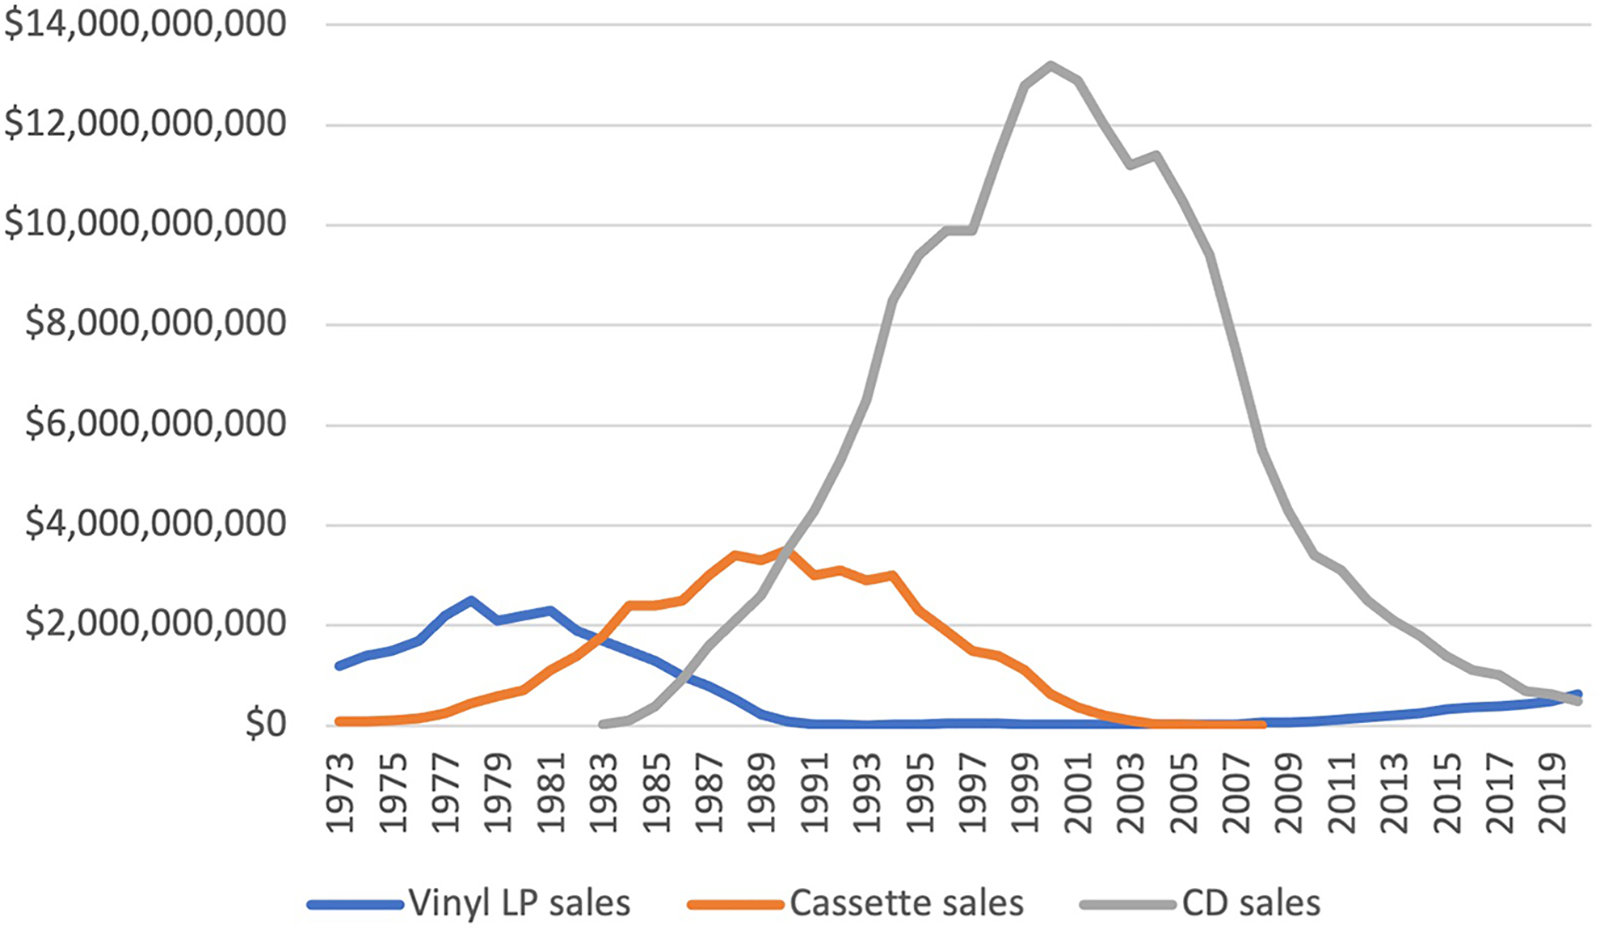
\includegraphics[width=\linewidth]{images/vinyl_sales_2023.png}
                \caption{Vinyl LP, Cassette, and CD Sales Revenue (1973–2020).}
                \caption*{Sourced from Journal of Popular Music Studies \cite{vinylRevival}}
                \label{fig:vinyl_sales}
            \end{figure}
    
            Although now taken for granted, records — and their predecessors, Edison's cylinders — transformed music from an ephemeral experience into a reproducible medium. Before recording technology, music was transient and confined to its place and time of performance, unable to be stored or shared beyond a live setting. While compositions could be transcribed into musical notation, each unique performance could never be heard again once it ended, unlike with visual art, where many original works from as far back as antiquity still survive \cite{jdbond}.
    
            This revolution in music consumption not only shaped the modern music industry but also cemented vinyl’s cultural significance. By making music ownable and replayable, it changed the way people engaged with it, fostering a more personal and enduring connection. Its enduring appeal, even in the digital age, suggests that its value extends beyond convenience, tapping into a deeper connection with music as a tangible experience.
    
            % Aesthetics
            \paragraph{Aesthetics and Emotional Appeal}
                % nostalgia, vibes
    
                Nostalgia plays a significant role in vinyl's resurgence. Statista data suggests the revival is primarily driven by two age groups: those aged 55+ and 25--34, with other demographics showing less engagement \cite{Gotting2021}. Older generations retain direct sentimental ties to the medium, while younger consumers are drawn to its cultural legacy.
    
                Despite the convenience of digital music, many consumers find it impersonal. In the past, music was a shared experience, often centred around a single household phonograph. Today, listeners frequently engage in isolated listening experiences \cite{historyandrevivalofvinyls}, with it being commonplace for multiple people in the same room to listen to different tracks at the same time. To an extent, music used to demand focus. You could not skip or replay a track without having to carefully reposition the needle. Some seek to reclaim the intentionality of music consumption, preferring a medium that encourages engagement rather than passive background listening \cite{Liu2020}.
    
                To many, music has become hollow- especially as music streaming services have easily monopolised the digital sphere \cite{historyandrevivalofvinyls}. Whether people are  yearning for the experiences of their past, or just a breath of `fresh air', many are turning to vinyl to do so.
    
                People are seeking community around their music and even its medium. Reddit's r/Vinyl, as of 2025, has over 2.2 million members. Whilst vinyl is still a relatively niche option, the social aspect of the internet means that, today, people are not confined to geographical constraints, and so, no matter how niche an interest is, they will be able to find like-minded people to connect to.
          
              % Ownership
              % Physicality
            \paragraph{Physicality and Ownership} % or MATERIALITY; general ethics
    
                Digital media ownership has become increasingly precarious, with consumers often purchasing revocable licenses rather than tangible assets \cite{verge2024steam_license}. This transition has upset many people, with there being many calls to bring back genuine ownership \cite{stanton2024gamers_pushback}, with legislation even being passed in California to make this fact more transparent to consumers \cite{california2024ab2426}.
    
                If a streaming vendor stops serving a particular piece of music, then that album can be lost to the public forever \cite{polygon2024cartoon_network_delisting}. However, if a consumer actually owns the physical discs or digital audio files, then they can ensure that they can listen to their audio, regardless of whatever licensing disputes may lead to the removal of digital media in the future (see \cite{bains2022lotr_strategy}).
    
                Furthermore, there are also concerns that streaming platforms often provide artists with minimal financial compensation, leading some consumers to purchase physical media as a means of direct support \cite{historyandrevivalofvinyls}. This means that there is a demographic of people who both own physical vinyls, but still make use of digital streaming services. Many even purchase physical vinyls despite not owning a device to play them on \cite{Trapp2023}. In addition, the act of gaining a physical good in support of an artist can even result in a psychological feeling of proximity to their idol \cite{historyandrevivalofvinyls}.
                
                Additionally, vinyl's finite nature contrasts with the boundless availability of digital tracks, making collections feel more meaningful and curated.
    
            % Audiophiles
            \paragraph{Audiophilia and Sound Quality}
    
                Another significant factor is the quality of the music being offered.
    
                \begin{quote}
                    \textbf{audiophile}: a person who is especially interested in high-fidelity sound reproduction. \cite{audiophile2025}
                \end{quote}
    
                % quality
                Vinyl is often perceived as superior in audio quality due to early digital compression limitations, such as the distortion issues highlighted in ``Tom's Diner'', wherein the a cappella's clean, isolated vocals revealed artifacts and distortions when encoded in early MP3 formats \cite{TODO}. Modern digital formats generally surpass vinyl in fidelity, particularly in bit depth and dynamic range. However, whilst advances in manufacturing storage drives have somewhat mitigated the need drastically to compress files, there are still valid use cases where extreme compression may be needed, such as for streaming audio on a low-quality network, which may cause the audio to sound worse than on vinyl.
    
                Additionally, as a physical format, vinyls are prone to being scratched and having physical deformities which affect the playback quality. Vinyl enthusiasts appreciate the medium’s imperfections, which are thought to add warmth and character. No two discs sounds exactly the same, whereas digital copies are utterly identical. This also creates a sense of personal ownership with vinyls - not only does the consumer own the physical disc itself, but they own their precise and unique version of it.
    
                It is important to note that many contemporary vinyl releases originate from digital masters, meaning potential losses in fidelity depend on how well an album is adapted to the format. Several inherent limitations affect vinyl playback, including: duration constraints, due to physical disk size; track sequence issues, as resolution gradually degrades towards the inner grooves; and RIAA equalisation, which alters frequency response to accommodate physical limitations of the medium \cite{engineeringvinyls}. Additionally, stereo information handling differs from digital formats, as vinyl relies on lateral and vertical groove modulation, which can introduce crosstalk and phase issues \cite{engineeringvinyls}. These factors, if not carefully managed during production, may compromise the listening experience - meaning modern tracks may often perform better in their original digital forms.
    
            \paragraph{Conclusion}
                While digital audio services offer notable convenience, the enduring vinyl revival demonstrates that many users still value tangible, nostalgic experiences. Nostalgia and charm play a crucial role in this appeal, making it essential to design with these emotional connections in mind. By combining the strengths of both physical and digital formats, a system can provide a richer, more meaningful user experience that aligns with modern consumption habits while preserving the authenticity and personal connection that vinyl enthusiasts cherish. A significant portion of consumers actively engage with both streaming services and physical media, indicating that a hybrid approach has a viable audience.
    
        \subsubsection{Image Recognition}
    
            \begin{temp}
                Y. LeCun and Y. Bengio, 1995, "Convolutional Networks for Images, Speech, and Time-Series". Brain theory neural networks, vol. 3361
            \end{temp}
    
            Image recognition is the creation of software and tools which can be used to identify objects, places, people, etc. in digital images, which has existed since at least 1946 \cite{hall1979computer}. However, in this brief time, the field has undergone several drastic changes as technology has advanced \cite{imagenetclasscnn}, and is still be redefined in the present day, particularly with the arrival of machine learning approaches, with new implementations being utilised across the field (e.g. \cite{RAMPRASAD2025100556}, 2025).
    
            \paragraph{Traditional Methods}
            
                Before the advent of deep learning, image recognition primarily relied on manually crafted feature extraction techniques. Classical methods included edge detection, template matching, and statistical pattern recognition. Notable feature descriptors such as Scale-Invariant Feature Transform (SIFT), Speeded-Up Robust Features (SURF), and Histogram of Oriented Gradients (HOG) played a significant role in object detection and classification \cite{pal2001pattern}. However, these approaches were often limited by their inability to generalise across variations in lighting, scale, and occlusions. The ImageNet Large Scale Visual Recognition Challenge (ILSVRC) served as a benchmark for evaluating the effectiveness of traditional and emerging techniques \cite{russakovsky2015imagenetlargescalevisual}.
            
            \paragraph{Emergence of Convolutional Neural Networks}
            
                The introduction of convolutional neural networks (CNNs) marked a paradigm shift in image recognition. Early work, such as LeNet-5, demonstrated CNNs' potential \cite{726791}, but it was the breakthrough of AlexNet in the 2012 ImageNet competition that solidified their dominance \cite{imagenetclasscnn}. Subsequent architectures, including VGG, ResNet, and EfficientNet, further improved performance by introducing deeper networks, residual connections, and optimised convolutional layers \cite{deppcnnsforimagerecognition}. These advancements enabled significant improvements in tasks such as object detection, facial recognition, and medical image analysis.
    
                In the context of vinyl cover art recognition, CNNs offer a powerful solution for identifying album artwork despite variations in artistic style, degradation, and distortions. However, a key challenge in training CNNs for this task is the limited availability of labelled datasets. Unlike large-scale image classification datasets like ImageNet, curated datasets for album cover recognition remain relatively small. To address this limitation, data augmentation techniques—such as random cropping, rotation, colour jittering, and synthetic distortions—help improve model robustness by simulating real-world variations \cite{LIN2025102660}. There has even been research done recently into using stable diffusion techniques to facilitate fully artificial data augmentation, with generative AI \cite{Alimisis2025}.
    
            \paragraph{Multi-Headed Networks and Consensus-Based Recognition}
    
                A limitation of conventional CNN models in image recognition is their reliance on a single decision pathway, which can lead to misclassifications when dealing with visually similar or degraded images. One approach to mitigate this issue is the use of multi-headed neural networks, where multiple CNN branches extract different features and contribute to a consensus decision. This technique allows the network to assess multiple aspects of the image, such as texture, dominant colours, and key object structures, before making a final classification \cite{Zheng2017}. 
            
                By integrating multi-headed architectures with ensemble strategies, models can achieve higher classification accuracy and robustness, particularly when handling ambiguous or visually noisy inputs. This method has been successfully applied in fine-grained classification tasks and could be adapted for vinyl cover recognition by leveraging multiple specialised feature extractors that assess distinct album cover characteristics.
    
            \paragraph{Current 'State of the Art'}
    
                Visual transformers currently represent the state-of-the-art in image classification, significantly outperforming traditional CNNs on large datasets. However, their performance heavily depends on large-scale data availability; with limited or specialised datasets, such as vinyl cover recognition, transformers may perform poorly or be impractical. Thus, CNN-based architectures or hybrid approaches remain more suitable in scenarios with smaller, niche datasets.
    
                A key challenge is ensuring models generalise effectively to unseen data, avoiding overfitting. Techniques like dropout, which randomly deactivate neurons during training, improve robustness by preventing reliance on specific features. Additionally, splitting datasets into training, validation, and test subsets enables monitoring model generalisation, though careful consideration is required to balance partition sizes and representativeness, whilst also avoiding biases. Data augmentation (e.g., rotations, lighting adjustments) further enhances performance by artificially expanding the training data, and improving generalisation by simulating real-world variations. However, larger augmented datasets increase computational demands, making GPU or TPU optimisations essential for efficiency.
    
        \subsection{Legal and Ethical Considerations}
    
          The training and use of machine learning models for image classification requires the acquisition and processing of data, which, in order to effectively handle the cover art of existing albums, necessitates obtaining and using their copyrighted artworks. This raises both legal and ethical concerns, particularly regarding compliance with UK copyright law and exemptions. This section examines the legal basis for dataset usage, fair dealing exemptions, and the ethical implications of using copyrighted material in an academic AI project.
    
              \subsubsection{Copyright Law and Fair Dealing}
                  % explain copyright law
                  Under the \textit{Copyright, Designs and Patents Act 1988} \cite{cdpa1988}, creative works, including album covers, are protected from unauthorised use, reproduction, distribution, and modification.
          
                  % introduce fair dealing
                  However, UK law also provides a key exception known as Fair Dealing, which allows limited use of copyrighted material under specific conditions, although such exemptions are only granted under very specific circumstances and for a very limited scope of use. Importantly, it is not a rigid rule but a context-dependent legal doctrine, evaluated on a case-by-case basis. The law does not explicitly define what qualifies as fair dealing; instead, courts assess whether a use is reasonable and justified based on the combination of several established legal factors.
                  
                  One of the most relevant exemptions is non-commercial research, as outlined in \textit{Section 29(1)} of the CDPA:
                  \begin{quote}
                      Fair dealing with a work for the purposes of research for a non-commercial purpose does not infringe any copyright in the work provided that it is accompanied by a sufficient acknowledgement. \cite{cdpa1988}
                  \end{quote}
    
                  This indicates that non-commercial academic research can be exempt from copyright infringement if proper attribution is provided. However, the applicability of this exemption depends on further and additional factors, such as the amount of material used and its impact on the copyright holder’s market.
    
              % 1. Using a dataset to create a model
              \subsubsection{Use of Artworks in Model Training}
              
                  Album covers are protected by copyright as highly creative works. Any reproduction or modification is typically restricted without permission from the copyright holder. As such, the bar needed for fair dealings is very high when dealing with such artwork. However, training a classification model may qualify for fair dealing, provided certain conditions are met.
    
                  A key legal question is whether machine learning training qualifies as ``\textit{computational analysis}'' under \textit{Section 29A} of the CDPA, which states:
                  \begin{quote}
                      (1) The making of a copy of a work by a person who has lawful access to the work does not infringe copyright in the work provided that—
                  
                          (a) the copy is made in order that a person who has lawful access to the work may carry out a computational analysis of anything recorded in the work for the sole purpose of research for a non-commercial purpose, and
                          
                          (b) the copy is accompanied by a sufficient acknowledgement (unless this would be impossible for reasons of practicality or otherwise). \cite{cdpa1988}
                  \end{quote}
    
                  This expresses that there is a strong argument for legal use of copyrighted materials in creating a computational model which classifies data by comparisons of analytically-derived embeddings.
    
                  It is, however, important to consider whether image processing qualifies as analysis under this law or whether this interpretation is too broad, given that past applications of computational analysis have predominantly involved text, and that image processing of this kind is still relatively new. Since there is no clear legal precedent on this specific topic (with changes being in the process of being made \cite{guardian2024uk_ai_copyright}), further legal clarification over the next few years will be necessary to definitively confirm or deny its applicability to image-based AI models. But, in the time before then, it can be used as a basis.
    
                  It also reiterates the need for attribution, but, notably states that this is only required in cases where it is feasibly practical.
    
                  Given these factors, classification likely qualifies under Fair Dealing because the model does not generate new images but merely classifies existing ones. This distinction is important, especially given recent scrutiny of generative AI models like OpenAI’s \textit{DALL·E} \cite{times2025christies_ai_auction, guardian2025ai_art_auction}, which create derivative works rather than merely labelling.
    
                  None of this is clear-cut, however, as we are still in an uncertain time with the law not having been stabalised after the emergence and mass adoption \cite{bick2024rapid} of these new technologies. It is worth noting, however, that there are currently proposals for UK law the explcitly allow the use of copyrighted materials in such cases \cite{guardian2024uk_ai_copyright}, whereas, in the US, there is starting to be legal prescendent of cases winning on the basis \cite{apnews2025thomson_reuters_ai_case} of AI agents using copyrighted data.
    
              % 2. Sourcing said dataset
              \subsubsection{Legal Compliance in Dataset Sourcing}
    
                  Beyond Fair Dealing considerations, data sourcing must be legally compliant. According to \textit{Section 29A} \cite{cdpa1988}, only individuals with lawful access to copyrighted works may use them for computational analysis. Therefore, it is essential to determine how these images can be legitimately acquired.
    
                  Machine learning models must fully process training images in their entirety to generate a model. This requires the whole image to be either stored persistently (on disk) or temporarily (in memory). Even if the image is only ever stored and processed in chunks (similar to how streaming providers serve video data), the overall image is eventually processed by the model. \textit{Section 28A} outlines more leniency for cases where only temporary copies are stored, for lawful access.
    
                  It is also important to consider if entire images are required, as opposed to only sections of them. If it would be possible to achieve the desired result using only subsets of the acquired dataset, then more data would be stored and used than is justified. The legal precedent \textit{Ashdown v Telegraph Group Ltd (2002)}, highlights that:
    
                  \begin{quote}
                      The third most important factor is the amount and importance of the work that has been taken . . . in some circumstances the taking of an excessive amount, or the taking of even a small amount if on a regular basis, would negative fair dealing. \cite{tmlocad}
                  \end{quote}
    
                  Thus, ensuring only necessary data is used is critical for compliance.
    
                  % 3. ToS compliance
                  In addition to just the handling of the data, however, its source must also be considered. There are three methods by which the training dataset could be acquired: by fetching data from an API, by scraping the data from the web, or, by manually taking the required photos (either by just me, personally, or by crowd-sourcing the images). Realistically, the first two options are most practically feasible.
    
                  There are many vendors of the cover arts of music albums. Notably, music vendors (such as \textit{Spotify}) and music collection and review sites (such as \textit{Discogs}) provide the album arts in a structured format where the artworks are synchronised with the albums which they belong to. However, due to the recent boom of generative AI models - and the controversy surrounding them \cite{apnews2025mccartney_ai_warning} - many vendors have explicitly prohibited the use of their data for machine learning in their Terms of Services.
    
                  % specific examples should probably be discussed under 'Design'
                  \begin{quote}
                      Do not use the Spotify Platform or any Spotify Content to train a machine learning or AI model or otherwise ingest Spotify Content into a machine learning or AI model.
                  \end{quote} \cite{spotifyDevPolicy} (III.14)
                  \begin{quote}
                      Do not misuse the Spotify Platform, including by i. using the Spotify Platform or any Spotify Content to train a machine learning or AI model or otherwise ingesting Spotify Content into a machine learning or AI model;
                  \end{quote} \cite{spotifyDevTerms} (IV.2.a.i)
                  \begin{quote}
                      [Discogs] strictly prohibit (1) the development of any software program, including, but not limited to, training a machine learning or artificial intelligence (AI) system using the Service content
                  \end{quote} \cite{discogsToS} (LICENSE AND SITE ACCESS)
    
                  However, if a site has more permissive policies, allowing the training of AI models, then, as long as the images are handled appropriately, they can be lawfully accessed and used.
    
              \subsubsection{Ethical Considerations}
              % Even if it's legally permissible, is it ethically responsible?
              % Does it impact the commercial success of artists?
              % Transparency & attribution concerns.
    
                  Even if it is legally permissible to source and use these images, it is also important to consider whether or not it is ethically responsible. These images, at the end of the day, are the highly creative works of artists, whose livelihoods come from their creations \cite{heikkila2022ai_art}. Reproducing (by downloading) and using their works therefore cannot be done without serious moral consideration.
    
                  Most significantly, it is worth noting that this AI model is not generative (which is where most of the recent controversies stem from \cite{apnews2025mccartney_ai_warning}), and therefore, instead of producing its own artworks based off of the images fed to it, it simply classifies them by labelling them with its prediction of their corresponding album. Therefore, whilst the model is technical derived from the artist's works, the produced work is not in competition with the additional artists - unlike generative agents \cite{times2025photographer_ai_copy} - and therefore should not have a negative impact on their commercial success. If anything, it is argued that this system should benefit them, by encouraging the purchasing of physical media, and garnering instances of playing their content on a revenue-generating service.
    
                  Furthermore, as this does not share or distribute the images themselves with the users, I believe it to be even more safe, as the only artefact generated from these images are a classification system which can be used by the user, but even the numerics themselves are not made accessible to the user.
    
                  And, whilst the law allows for the exclusion for explicit attribution of all involved copyright holders, this may not be ethical. However, as this is a classification system, it arguably gives some degree of implicit accreditation to the artworks used in the training process, when the predicted label is used to redirect the user to said album.
    
              \subsubsection{Conclusion}
    
                  This section examined the legal and ethical implications of using copyrighted album covers in machine learning. Based on UK Fair Dealing exemptions in the CDPA 1988, I would argue that there is a solid grounding this project likely qualifies as a legally permissible use case, provided:
                  \begin{description}
                      \item[-] It is a non-commercial, research project.
                      \item[-] Data is lawfully acquired from permitting sources.
                      \item[-] The dataset scale and usage is minimised to strictly what is neccessary.
                      \item[-] None of the images are shared or modified. % this will need to be checked when talking about data augmentation
                  \end{description}
                  
                  From an ethical standpoint, the project is distinguishable from controversial generative AI models, as it does not replace artists’ work or impact their revenue streams. Nonetheless, transparency and attribution best practices should be followed.
    
    %%%%%%%%%%%%%%%%%% SECTION 3 %%%%%%%%%%%%%%%%%%
    \section{Design} % DESIGN / METHODOLOGY
        \begin{temp}
            What did past-Jack set out to do? Here should be the broad vision, including the change of direction taken.
        \end{temp}
        % design diagrams!
    
        Initially, the project was envisioned to be a native desktop/mobile application, with a goal of supporting a range of devices. Since, for many, music is now a personal and individual consumption, bringing the idea of the vinyl system into one's pocket seemed like the most practical and intuitive approach. Furthermore, since having a portable system would allow for an incredibly large and diverse range of albums being scanned, it was decided to use streaming services and APIs in order to maximise the breadth of the available 'library' for the application. Since this initial design focused on being device-agnostic and using live audio streaming, it was decided that a web architecture was most fitting, as frameworks already exist to serve web content on various devices, and because most audio APIs/SDKs require (or work best with) these technologies. Prior experience with Android Java development and the Spotify Web and Android SDKs, specifically, also made this an appealing decision.
    
        However, shortly into the development period, since the background research showed that there is a strong attraction of existing vinyl users for the medium due to its physical nature: it was decided to instead create a single physical device, whilst still utilising online music streaming. This would still allow it to have the convenience of a digital player with easy library availability and playing to the strengths of virtual playback for modern tracks, whilst also encouraging the ownership of physical mediums, and leaning into the physicality in its design and interaction mechanisms. Additionally, the research showed that there is an existing demographic of consumers who purchase both physical and digital copies (or subscriptions) simultaneously - making this combinatorial design viable with a target audience of consumers. Despite being a single, localised device, in order to integrate the streaming services seamlessly, it was still required to use a webstack, and so, the design became to run both the server and client on the same device, locally. Deviating from the exact technologies used in a previous project was also seen as a good opportunity to develop new and additional skills and familiarity with other technologies.
        
        \subsection{Requirements Analysis}
            % list of requirements
    
            \begin{temp}
                UML Use Case Diagram
            \end{temp}
    
        \subsection{Pillars of Design Philosophy}
    
            Some core principles were adopted in the design phase:
    
            \begin{itemize}
                \item \textbf{Platform Agnosticism} A core design philosophy of the project was to, where possible, make the system as robust as possible by preventing it from becoming overly reliant on any one external component. This was largely done by implementing the system through 'hexagonal programming' (or, 'plugs and adapters') techniques, allowing components to conform to common interfaces, such that they could be easily switched, on demand. In addition to just being flexible for services, it was also a priority to make the application accessible across a multitude of devices; supporting as many OSes and architectures as possible.
            \end{itemize}
    
            \begin{itemize}
                \item \textbf{Physicality First} The device should lean into its physical nature, and, where possible, utilise this, to best make use of the nostalgia and enjoyment people have for physical vinyl players.
            \end{itemize}
    
            \begin{itemize}
                \item \textbf{Digital Completeness} Whilst the system was designed to function with physicality first and foremost, a secondary core design principle was to make everything the physical components could do also be achievable through digital means. This is particularly important to consider so that those with physical impairments are still accommodated for and not marginalised by the system.
            \end{itemize}
    
            \begin{itemize}
                \item \textbf{Open Source} Whilst not inherently imperative for most design decisions, with a firm belief in the importance and value of the open source community, it was decided that this project would a contributor. Under the confirmation that publicising the code for the project in its entirety would not be in infringement of academic malpractice rules, the repository was made public. Additionally, open-source offerings were favoured, where possible, when selecting which services and technologies to use.
            \end{itemize}
    
            \begin{itemize}
                \item \textbf{Robustness and Maintainability} Writing clean, modular, and maintainable code was emphasised from the outset. The use of established design patterns, adherence to the Single Responsibility Principle, and rigorous unit testing practices help ensure reliability, ease of maintenance, and facilitate future enhancements.
            \end{itemize}
    
            \begin{itemize}
                \item \textbf{Ethical Responsibility} The project was developed with ethical considerations at the forefront, particularly regarding copyright compliance, transparency, responsible data usage, and awareness of broader social impacts. This also extends to having an intentional approach in making the system secure and safe.
            \end{itemize}
        
        \subsection{System Architecture} % high-level system overview
    
            \begin{temp}
                Here should be \textbf{descriptive} elements as to what was decided for the final design.
            
                System Architecture Diagram \ref{fig:networkDiagram};
                \begin{temp}Note from Sean: Discogs/Spotify should be together\end{temp}
                
                Data Flow Diagram; Component Diagram;
    
                Hexagonal Architecture (Ports \& Plugs); (modularity = Single Responsibility Principle)
    
                Single-page application
            \end{temp}
    
            The final architecture design was to create a web application with a single, central server running on the physical device, that could be interfaced with from both physical analogue controls, in addition to exposed REST endpoints. This same device would also locally run a web client in order to stream the audio and display visuals for the user, communicating through the server with both traditional server calls, but, also, a bi-directional Websocket connection, allowing both the server and client to instantaneously broadcast to each other.
            % This broadcasting mechanic is useful, as it allows the server to inform the client of state changes, such as if the audio should be paused due to a physical button being pressed.
    
            The device was designed to use a motor to spin a disc during playback -- to replicate how an original vinyl system spins the vinyl itself -- and the host client's interface would be projected, vertically-downwards onto the system, making the physic disc be textured like a vinyl, whilst also giving live information such as the current user in a holographic-like style.
    
            It was later decided, further into development, that the network architecture should be extended to allow for 'remote clients' (that is, devices other than the main one running the server) to also connect, in order to allow easy and communal remote control of the device. In order to accommodate this, the server was updated to handle multiple websocket connections simultaneously (see Figure \ref{fig:networkDiagram}).
        
            \subsubsection{Design Choices}
                % unique 1-1/1-many relation
                % server hardware control
                % host v. remote client
                \begin{temp}
                    Here should be the \textbf{justificatory} elements for the choices made: particularly the more broad, or weird, or niche choices. Very specific logical choices should be in their specific components.
                
                    For example:
                    \begin{description}
                        \item[1.] Why use a web approach for a localised device?
                        \item[2.] Why use an unorthodox 1-1 Websocket approach for client-server calls?
                    \end{description}
                    Also things such as 'point of truth handling', etc.
    
                    Is it a good idea to write this explicitly like an FAQ section, with the question stated, and then answer given?
                \end{temp}
    
                \paragraph{Why use a web approach for a localised device?} Despite being an application initially designed to run on a single-device, a webstack solution was still used. Whilst this seems slightly unintuitive, it maximised the options when selecting a streaming service to implement, since, as streaming services, they rely on web technologies. In addition to this, it made the application inherently device-agnostic. Furthermore, when the decision was made to allow remote device to connect, the existing web architecture made this a seamless addition, since it was already configured, and network hosting removed the need for any per-device configuration. 
    
                \begin{figure}[h]
                    \centering
                    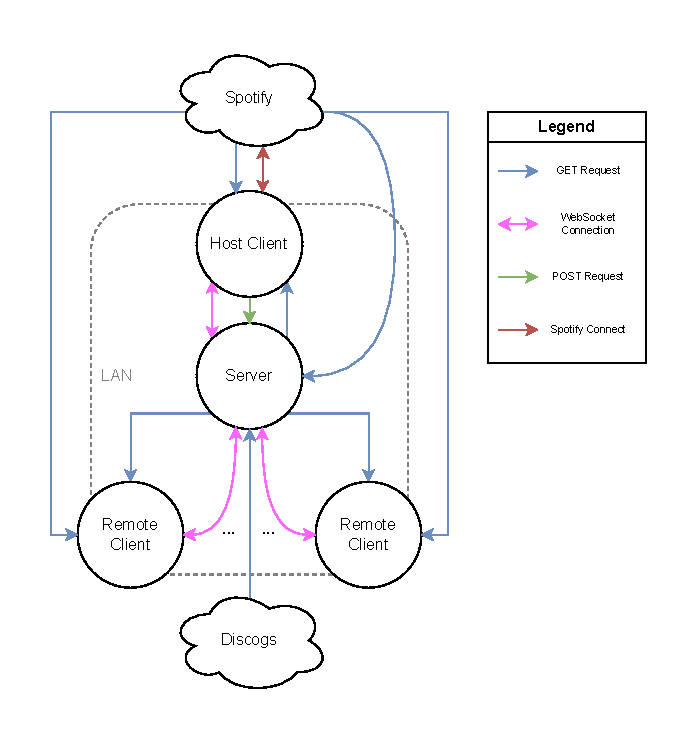
\includegraphics[width=\textwidth]{images/VTT_network.NetworkDiagram.pdf}
                    \caption{Network diagram of system. }
                    \label{fig:networkDiagram}
                \end{figure}
        
            \subsubsection{Technology Stack}
    
                This project utilises a range of technologies, each chosen for their relevance to the project’s requirements:
    
                \begin{temp}
                    Is this actually needed? All of these things are covered below. But, it seems good to have a concise high-level summary?
                \end{temp}
                
                \begin{itemize}
                    \item \textbf{Music Vendor:} Spotify Web Playback SDK --- used as the main audio stream provider. Spotify was chosen due to the existing Premium subscription requirement, unlike alternatives (e.g.\ Apple Music). Prior experience with the SDK also influenced this choice.
    
                    \item \textbf{Frontend:} React, TypeScript --- used to support streaming SDKs. TypeScript ensures type safety, while React provides efficient reactivity to data changes from multiple sources.
                    
                    \item \textbf{Backend:} Python, FastAPI --- selected for its strong machine learning library support and familiarity. FastAPI was chosen for its simplicity, lightweight nature, and ease of use.
                    
                    \item \textbf{Build Tool:} Bun \& Vite --- Bun was chosen for its speed, with Vite used on top to enable rapid testing and network hosting.
    
                    \item \textbf{Hardware:} Raspberry Pi 5 --- a Raspberry Pi board was chosen for easy GUI interfacing with simultaneous modularity for physical components; the latest board available at the time was used to maximise performance of the neural network.
                \end{itemize}
    
        \subsection{Hardware}
    
            It was decided to run this system on a Raspberry Pi 5, in order to have a flexible and easy-to-use system, whilst still having decent processing power for the neural network. Microcontrollers such as Arduino boards were considered, however, since the software was designed to be usable on any reasonable device, it needed a device that could run a general-use OS and web browser. The NVIDIA® Jetson Nano™ Developer Kit was considered, as it is a powerful AI-oriented chipboard, featuring an NVIDIA Maxwell architecture with 128 NVIDIA CUDA® cores. For running a neural network solution, this architecture is significantly more powerful than the Raspberry Pi 5's equivalent VideoCore VII GPU, which is primarily for graphics and not general-purpose GPU compute like CUDA. However, this superior computing comes at a more significant price than the Pi, and, whilst it would be more capable at running ML models, using the less specialised Pi necessitated good optimisation practices, better ensuring that the final product should function well on a range of systems.
            
            However, rather than just running the device, aesthetics were considered. In order to best utilise nostalgia, the device was designed to make use of a stylish mahogany wood with brass controls. Research shows that, in one survey, wood is the most frequently cited material in nostalgic household items, appearing in 34\% of nostalgic objects (with metal second at 21\%) \cite{Skinner2022}. These materials were ubiquitous in classic mid-20th-century audio equipment, so they instantly call to mind ``the charm of a bygone era'' \cite{LookInTheAttic2024}.
    
            \subsubsection{Hardware Components}
    
                During the design phase, it was crucial to ensure the chosen hardware components could be accommodated by the Raspberry Pi's limited number of GPIO pins, some of which have specific functionality constraints (see Figure \ref{fig:RPi5Pinout}).
    
                \begin{figure}[htbp]
                    \centering
                    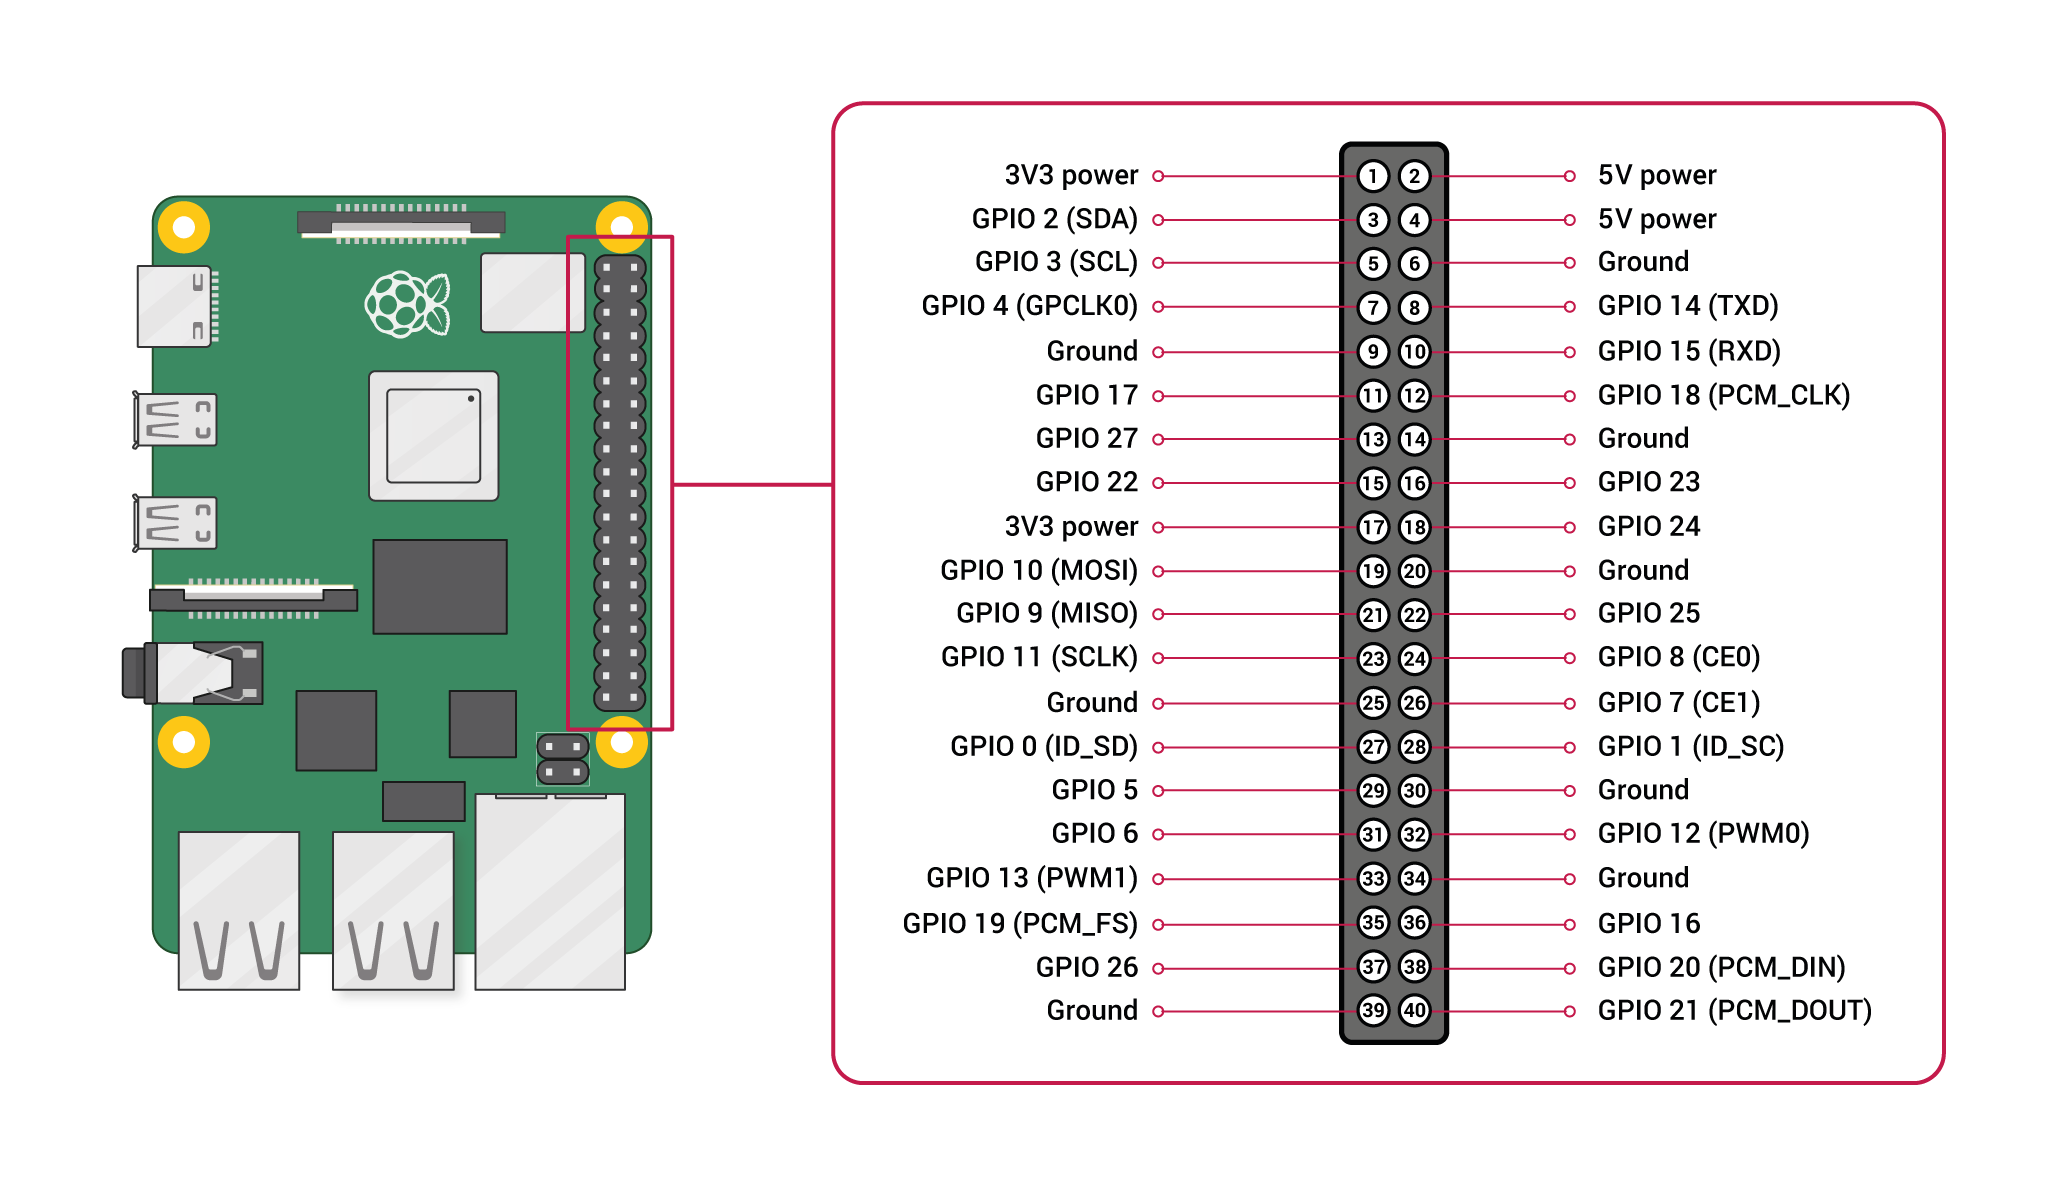
\includegraphics[width=\linewidth]{images/raspberry-pi-5-pinout.png}
                    \caption{Pinout configuration of Raspberry Pi 5}
                    \label{fig:RPi5Pinout}
                    \caption*{Source: \href{https://www.raspberrypi.com/documentation/computers/raspberry-pi.html#gpio}{Raspberry Pi Documentation}}
                \end{figure}
    
                It was decided that the core functionality could be covered by a motor driver, a DC motor, a rotary encoder switch, a button and a single camera (see Table \ref{tab:coreGPIOPins}). This would allow the device to capture images to process through the camera, which can be manually triggered with the button. The rotary encoder switch allows rotational vector input (direction of clockwise or anticlockwise, with magnitude), in addition to a single press-button -- these elements can be combined to fully handle playback control (play, pause), track skipping (previous, next), and volume control, by using a combinatorial solution that tracks rotation in relation to if the button is pressed. For example:
    
                \begin{itemize}
                    \item \textbf{Knob rotated, button not pressed}: Change volume up or down, depending on direction and amount.
                    \item \textbf{Button pressed, no rotation}: Toggle pause/play.
                    \item \textbf{Knob rotated, button pressed}: Change track to previous/next, depending on direction.
                \end{itemize}
    
                \begin{table}[htbp]
                    \centering
                    \caption{GPIO Pin Requirements for Core Functionality}
                    \label{tab:coreGPIOPins}
                    \begin{tabular}{|l|l|l|}
                        \hline
                        \textbf{Component} & \textbf{Required Pins} & \textbf{Note}\\ \hline
                        \multirow{5}{*}{DC Motor (via Driver)} & 1 × 5\,V & Motor driver power \\ \cline{2-3}
                                                               & 1 × GND & Ground \\ \cline{2-3}
                                                               & 1 × 5\,V & Motor power \\ \cline{2-3}
                                                               & 2 × GPIO & Direction control \\ \cline{2-3}
                                                               & 1 × GPIO (PWM) & Speed control \\ \hline
                        \multirow{5}{*}{Rotary Encoder Switch} & 1 × 3.3\,V & \\ \cline{2-3}
                                                               & 2 × GPIO& Rotation data (CLK, DT)\\ \cline{2-3}
                                                               & 1 × GPIO & Button input (SW)\\ \cline{2-3}
                                                               & 1 × GND & \\ \hline
                        \multirow{2}{*}{Button (Camera Trigger)} & 1 × GPIO & \\ \cline{2-3}
                                                                 & 1 × GND & \\ \hline
                        Camera & 1 × USB or Ribbon Port & \\ \hline
                    \end{tabular}
                \end{table}
    
                However, ideally some additional features were desired, such as having a more physical interaction mechanism, using a hinge switch; a rotary encoder to monitor the device's motor; and a secondary camera to capture images of the back of a vinyl, as well as the front (see Table \ref{tab:optionalGPIOPins} for details). Having a large 'arm' that hinges and requires more physical movement would allow for users to have both a more simple mechanism for controlling the pause/play state of the system, whilst still allowing the freedom to choose to use the knob, if desired.
    
                \begin{table}[htbp]
                    \centering
                    \caption{GPIO Pin Requirements for Optional Components}
                    \label{tab:optionalGPIOPins}
                    \begin{tabular}{|l|l|l|}
                        \hline
                        \textbf{Component} & \textbf{Required Pins} & \textbf{Note}\\ \hline
                        \multirow{5}{*}{Rotary Encoder (Motor Stall Detection)} & 1 × 3.3\,V & Sensor power (VCC)\\ \cline{2-3}
                                                                                & 2 × GPIO & Rotation data (A, B) \\ \cline{2-3}
                                                                                & 1 × GND & \\ \hline
                        \multirow{2}{*}{Hinge Switch} & 1 × GPIO & \\ \cline{2-3}
                                                      & 1 × GND & \\ \hline
                        Secondary Camera & 1 × USB or Ribbon Port & \\ \hline
                    \end{tabular}
                \end{table}
    
                Additionally, adding a rotary encoder to the motor would allow for stall detection, which can prevent burnout if the motor is being forcibly stalled, increasing the longevity of the component.
                % In addition to this, a camera was needed for the scanning. It was decided to use a regular USB webcam, as opposed to the standard RPi camera modules, to further prevent dependance on RPi solutions.
    
                As per Table \ref{tab:pinSummary}, the above core and optional requirements can all be accommodated by the board's available pins and ports, whilst leaving a reasonable number of redundant pins in case of any issues that arise, or potential expansions. The exception to this is 5\,V power pins, which would be at full capacity; though, if there is any issue or need for more of these, the motor can instead be powered through the motor driver with an external battery, freeing up a pin. 
    
                \begin{table}[htbp]
                    \centering
                    \caption{Summary of GPIO and Port Requirements vs. Availability}
                    \label{tab:pinSummary}
                    \begin{tabular}{|l|c|c|c|c|}
                        \hline
                        \textbf{Pin / Port Type} & \textbf{Core}& \textbf{Optional}& \textbf{Total Required} & \textbf{Available} \textsuperscript{see Figure \ref{fig:RPi5Pinout}
    }}\\ \hline
                        5\,V Power & 2 & & 2 & 2 \\ \hline
                        3.3\,V Power & 1 & & 1& 2 \\ \hline
                        GND & 3 & 2 & 5 & 8 \\ \hline
                        GPIO (Standard) & 6 & 3 & 9 & 28 \\ \hline
                        GPIO (PWM-capable) & 1 & & 1 & 4 \\ \hline
                        USB or Ribbon Port & 1 & 1 & 2 & 2+\textsuperscript{*}\\ \hline
                    \end{tabular}
                    \caption*{\textsuperscript{*}Raspberry Pi 5 supports 4× USB + 2× camera ribbon ports.}
                \end{table}
    
            \subsubsection{Operating System}
    
                Raspberry Pi OS (or just RPiOS; formerly Raspbian), is an operating system produced by the the Raspberry Pi Foundation as the official OS for their chipboards. This makes interfacing with components such as GPIO pins seamless and easy. However, in order to make the system as hardware-agnostic as possible, a standard Ubuntu kernel was used for the project. This forced solutions to not rely on native Raspberry Pi interfaces, and so, whilst it made certain aspects more challenging, it means than the project is not locked to the RPi hardware.
    
                Additionally, Ubuntu is fully open-source, whereas RPiOS has some proprietary aspects.
    
                For running the interface, Firefox (an open-source non-chromium browser), as Ubuntu's default browser, was used for primary development. However, the application was also periodically tested on chromium, to ensure compatibility with other browsers.
        
        \subsection{Front-end}
            \subsubsection{Primary User Interface}
                % lofi designs
    
                \begin{temp}
                    - Physical user interaction controls
                \end{temp}
    
                \begin{temp}
                    UI Wireframes / Mockups
                \end{temp}
    
                The initial aim to create a device-agnostic platform made web technologies an ideal choice, and out of the available frameworks, React was selected due to having good support for reactive UI updates from multiple sources. This feature is especially useful, as the host client application is responsible for interfacing with the streaming service(s), and needs to handle state changes from not only its own UI controls, but also from the vendor itself, and from the server's websocket connection which relays commands from the physical controls and from remote devices (see Figure \ref{fig:statePropagationDiagram} for the different sources of state changes). In addition to this, prior experience with the framework was also an influence.
            
            \subsubsection{Audio Playback}
                % Spotify Playback SDK
                % Spotify Web API
    
                In order to keep with the goal of being platform-agnostic, all API connections for the music playback and metadata retrieval was done through object-oriented programming interfaces and abstract classes, forcing all implementations to inherit and conform to these, enforcing uniformity and allowing the interfacing system, such as the host client, to seamlessly use any of them, as a black-box system.
    
                However, for this project, only one external streaming API was selected to be implemented. After considering various options, Spotify was chosen due to past experiences with the system making it faster to integrate. In addition, most services required a subscription with the service in order to stream them; a pre-requisite already met for Spotify. For these reasons, Spotify was chosen for the audio streaming in the front end component, and thus, the corresponding back-end systems also used Spotify.
    
            \subsubsection{Minimal UI}
    
                Once it was decided to create a single physical device, the emphasis became to use physical controls over virtual UI buttons, where possible. A primary goal was to make the interface be entirely usable without the need for a mouse or keyboard (or even a screen), once configured. In order to emphasise this, the host client system was designed to be as minimal in UI components as possible, such that it would essentially be in a read-only state -- only showing data, and not controls, unless explicitly requested. To achieve this, buttons and sliders are hidden on the host client, unless the mouse was recently in motion.
    
                However, once the user indicates they are interfacing through the client, by moving the mouse, it was important to ensure that the UI offered no less control and/or information as the physical controls did.
    
                In addition to playback controls, the host client also has access to settings, which are fed to the server. These settings control who can remotely access the system (if at all), as well as making the motor component optional by disabling it. These options are provided exclusively on the host system.
        
            \subsubsection{Remote Clients}
    
                \begin{temp}
                    - for convineince, the need for (33-45) adapter  can be cited
                    % https://external-content.duckduckgo.com/iu/?u=https%3A%2F%2Fnotesonvinyl.com%2Fwp-content%2Fuploads%2F2022%2F04%2Fspeeds-of-the-different-record-types-1.png&f=1&nofb=1&ipt=7d1e31af8468ae7ae70f11be6bd40c897a73cf0c42aa194a5e09309f9af25945&ipo=images
                    % https://external-content.duckduckgo.com/iu/?u=https%3A%2F%2Fwww.bluescentric.com%2Fimages%2Fproduct%2Flarge%2F557_2_.jpg&f=1&nofb=1&ipt=1cd939744050d9f13eb7f581b786a2f22d3787cf30dd60c2a6975a816043546f&ipo=images
                \end{temp}
    
                During development, it was decided to not only allow a web browser to locally connect to the server, on the host device, but to expand the system to allow 'remote devices' such as external mobile phones and computers. This was decided on the basis of both accessibility and general convenience. As people with physical conditions could struggle to use physical controls, a remote connection from a phone would allow them still be able to operate the device. In addition, this also provides technological accessibility, as those without the required hardware (such as a camera) would be able to now use their phone's camera, to scan albums, as needed.
    
                This could also be used to bring a further communal aspect, as multiple people could connect to, and use, the device simultaneously, allowing an authorised individual to control playback or enqueue a song to share with the host and others. An additional benefit being that a user could upload a photo taken when away from the host device, allowing the initial portability design to not be entirely lost, even with the now-static system.
    
                Rather than implement a separate front-end or routing system, the client is a single-page application, using calls to the server to determine if the device is the host or external. The client then displays the correct form of UI to the user.
    
                The remote client UI includes buttons to play, pause, skip and return to previous tracks; it provides a volume slider; displays the album art of the track; allows scanning of an album; and even displays to the user the host's library of previously-scanned albums, which can be set to play individually, or shuffled as a whole collection. These controls allow the remote user to do everything a user physically interacting could.
        
        \subsection{Back-end}
    
            In order to allow multiple devices to connect with the host device, a centralised server system was needed. Not only would this server be responsible for handling communication between its clients, but it would also need to handle the physical control system, the album detection logic (discussed separately in Section \ref{sec:mlDesign}), authentication (see \ref{sec:security}) and any additional logic.
    
            Python was selected as a robust and easy-to-use high-level language to best accommodate all of these; especially since it has a very rich suite of machine learning libraries. FastAPI was selected as the framework for the server, using Uvicorn, as this is known for being fast and lightweight, ideal for the SBC.
    
            The server was created using the singleton pattern, to ensure that the machine learning model(s) are only initialised a single time at startup and across all requests, for optimal performance. Whilst parallelisation and scalability were not goals for this project, in order to achieve the goal of creating a robust solution, this bedrock layer of good practice was implemented.
    
            The server follows the Single Responsibility Principle, meaning functionalities are broken down into classes with each one handling one, and only one, functionality. This makes the REST endpoint routing, for example, easily separable from the APIs' logic, and from the authentication protocols. This design ensures the code is more readable and maintainable.
    
            As the server also handles the physical controls (in addition to needing to relay commands from the remote clients), the server needed to be able to instantaneously communicate with the host client. Rather than relying on inefficient polling, or the one-way, text-only approach of using Server-Sent Events (SSEs): websockets provide great flexibility in allowing the client and host to both communicate with each other, bi-directionally, with minimal delay and resource usage. This is ideal, because whilst the server will sometimes need to update the client (when a user uses a physical control, for example) there will also be times where the client systems need to update the server (for example, if the music is paused directly through Spotify, from a device not even connected to our server, the server needs to be informed of this by the host client). Using this bi-directional channel ensures that all similar communications go through the same context, and avoids needing to implement similar code multiple times, in different ways (such as if this was done with standard REST calls and SSEs).
        
            \subsubsection{Metadata Retrieval}
                % Discogs API
                % assert Discogs ToS compliance (not used for AI)
    
                Traditionally, when a track or album is playing, online streaming services show the cover art to the user. Since this project relies on scanning a cover art in order to play the music, it seemed redundant to broadcast the current track by showing the user the same artwork they have in their hands. So, in order to lean more into the physical vinyl concept, the server was designed to fetch the centre label of the corresponding vinyl, in order to show this on the disc, instead.
    
                In order to fetch this, Discogs' API was used, as they maintain a carefully curated library of many images for vinyls, including high-quality images of these labels. Whilst Discogs do not allow their images to be used in AI systems, these images are never fed into the machine learning model, and are strictly processed by traditional CV methods.
    
                The system was designed to simply, upon playback of a track, fetch images from the Discogs library, and find the best-matching circular image, using Hough Circle detection, and then cropping the image to serve to the front-end.
          
        \subsection{Machine Learning Model Design} \label{sec:mlDesign}
    
            In light of the background research, it was decided that using a machine-learning neural network approach would be better for this project, rather than traditional tailored OCR solutions (as some albums feature no text) or feature extraction techniques (as albums vary greatly, and manual defining features would likely yield worse  results). Whilst visual transformers are often the best performing models for large datasets, it was decided to use a smaller CNN, to better converge on the smaller and more specific dataset of albums.
        
            \subsubsection{Dataset Collection}
                % use of CoverArtArchive
    
                In order to train the model, a dataset of albums was required. Manual collection of images would be a slow process, and could introduce bias, when testing. Whilst there is wide abundance of these images on platforms such as Spotify and Discogs, their terms strictly prohibit the use of their served content from being fed into AI systems.
    
                One option was Last.fm, whose terms had no explicit prohibition of these use cases, and so was subject only to copyright law and fair dealings.
    
                However, the Internet Archive's (in collaboration with Musicbrainz) Cover Art Archive provides its images, with no restrictions on AI systems, either. In addition to being a viable option, this library also provides images of the backs of albums, which none of the other surveyed systems did, and, is an open-source solution, and so was selected to be the primary source of dataset collection.
    
                However, manual images were still collected to add to this dataset. This was essential to ensure that model validation could be done without bias (see \ref{data:val}).
    
            \subsubsection{Solution Design}
    
                The high-level solution to the album detection problem was to use the model trained on album images to classify which album was being scanned. In addition, the model should ideally be able to detect when the input image is not of an album at all,  for example if the camera was triggered too early, before the vinyl was placed. This could be done by feeding random images in during training as a 'null' class.
    
                If classification for this null class worked well, the camera could essentially poll images, and only react to high-confidence changes in its state, minimising the need for a user to press a button or other control to trigger the scan.
    
                However, rather than rely solely on the CNN mode, as a fallback system, it was decided to use the model to classify, and in cases where the model could not confidently give a prediction, it would use an OCR system, as a second attempt. In addition to OCR, barcode scanning was also decided to be used. This combinatorial approach was envisioned to make the model more robust at recognising images outside of the scope of its training data.
    
                \begin{temp}
                    Decision Flowchart for Image Recognition
                \end{temp}
        
            \subsubsection{Model Architecture}
    
                Based off of the research, it was decided to use a convolutional neural network, due to their excellence in image classification tasks.
    
                An educational approach was taken in designing the models, wherein the goal was to create a fully self-made solution with a simple architecture. Then, the model would be expanded upon and deepened, as needed, to get the best results, through experimentation informed by the literature.
    
                The goal was to create a few different models, with differences in architecture to experiment to find results. Other than broad decisions, their architectures were not developed until during implementation. The details of each of these models is described in Section \ref{sec:mlImp}.
    
                However, the conceptual models are described below. In order to distinguish between these models beyond just their most basic architecture, each was given a unique name. The inspiration for these names were taken from Greek mythology, and therefore each model is named after a mythological snake-creature (see Appendix \ref{app:Greek}, for more details).
    
                \paragraph{Ouroboros} A standard feed-forward CNN.
    
                At this most basic level, the goal is to simply design a model that can accurately learn information from both a small and large dataset of albums, to ensure that it can handle varying collection sizes of different users.
    
                Since the task of learning albums from their artworks is a closed-world scenario -- that is, the model is expected to classify inputs that are nearly identical to the training examples, with minimal variation, since two versions of the same album usually have identical artworks -- the need for generalisation is low and the model can rely more on memorisation. This `memorisation-friendly' nature of the task was the inspiration for the name Ouroboros, the self-eating serpent.
    
                \paragraph{Amphisbaena} A two-headed neural network, trained to capture and classify an image's most likely artist, in addition to the album itself.
    
                If the Ouroboros model is viable, then it was desired to experiment with adding multiple heads, so that the model could predict an artist, even if it had not been trained on a specific album. If an artist can be predicted with high confidence, but no album is overly confident, then this could be used to inform the search alongside the OCR/barcode data, etc.
    
                Additionally, through further experimentation, this could be expanded to learn genre, or even the decade of release.
    
                \paragraph{Hydra} An adaptive multi-headed model, allowing the creation of new heads through knowledge distillation and consensus to learn new, previously out-of-scope classes, whilst still maintaining precision on previously trained data.
    
                A significant issue with using a closed classification system (that is, it only trains once), is that any classes not included inside the training dataset can never be predicted. Whilst it is common practice to re-train (or fine-tune) a model, to adjust weightings based off of new data, the task of adding a whole new class to the model's options when deciding is a much more complex task.
    
                The most simple option is to simply re-train the whole model, with the additional classes and data. However, in order to best maintain fair dealings, all images used in training were deleted after use, by the system. Therefore, unless the user was to re-download the entire dataset each time, this was not a very viable option. Additionally, it could be the case that the online source of images may have had images removed, and therefore, re-training could actually offer worse performance in some cases.
    
                An aspiration target of model development for this project was to create a progressive neural network (PNN) that could adapt to new classes. The simple goal would be for the model to support a dynamic number of heads, and when new classes are added to train a new head using knowledge-distillation from previous heads (to prevent 'forgetting' previously trained classes), whilst still associating with the new classes. Once the new head is trained, it can be appended to the model, and a weighted consensus of the various heads would be used to determine the class.
    
        \subsection{Security Considerations} \label{sec:security}
            % handling of auth tokens (transient)
            % off-handing of persistence tasks
            % network hosting
            % option of same-user or any-user controls
            % API compliances
    
            \begin{temp}
                Security Architecture Diagram
            \end{temp}
    
            \begin{temp}
                Data Flow Diagram
            \end{temp}
    
            Whilst this system is designed as a local device, with the only connectivity to external sources being trusted APIs, security was still an important consideration, and taken seriously within each phase of the project.
    
            \paragraph{Handling of secure data} Since this project integrates with external systems, proper authentication token handling was required. Especially when serving multiple users simultaneously. The system follows a standard RESTful token flow, wherein a client is redirected to the server through the external service's callback, with a token that can be used to request a formal authentication token. This token is stored only in the server's memory, and is associated with the client's session ID cookie. Therefore, a user can only fetch an authentication token through the GET endpoint if they are the same device that made the request. This ensures secure data was only accessible to authorised parties.
    
            \paragraph{Persistence task off-handing} Some tasks require non-volatile storage, for example: storing a list of the albums a user has scanned into their 'collection'. The decision was made that, where possible, non-sensitive data should be off-loaded onto the API service being used. That is, rather than store the list of songs locally, a Spotify playlist can be created and updated as the system's 'file'. This meant all GDPR compliance needed to be met by the external vendors, rather than this system.
    
            \paragraph{Local network hosting} To handle remote clients, it was decided to allow the front-end runner (Vite) to use a feature called network-hosting. This feature allows LAN devices to connect to the site. Whilst opening access to certain ports to same-network devices can have consequences, as a static device, this system is designed to only be used in a secure network (such as the user's house), and so no major actions were taken, beyond ensuring firewall services did cover the relevant ports.
    
            \paragraph{Command permissions} It was decided that even if user A was signed in on the host device, user B should be allowed to pause, play, scan, etc. from their external device if, and only if, user A authorises this. To achieve this, not only are the required UI buttons disabled when the host has disabled remote access, but all server-side logic enforces this. The host can either disable all remote connection, or allow only the host's account to do this, or allow all devices to access the server. The validation for is a user is the host or not, is done through the session ID cookies and verifying with the external API that the associated token is for the authorised user. Therefore, this cannot be ignored by a malicious user.
    
            \paragraph{API compliances} An intentional effort was made to ensure that all data processing, requests, and request-frequencies were compliant with the respective APIs' terms of services, rules, and limitations.
        
        \subsection{Testing Methodology}
    
            \begin{temp}
                Design of tests and evaluations; plan for unit testing, model evaluation, etc.
                
                Does the system satisfy that physical and aesthetic desires of that the vinyl trend appeals to, whilst still offering functional convenience over original systems?
            \end{temp}
            
            \subsubsection{Validation of Effectiveness}
    
                In order to evaluate if the developed solution is effective in reaching its goals, three primary metrics will be used:
    
                \paragraph{Model Performance} In order to assess if the model performs adequately, formal model evaluation will be performed. Two units will be under test: the recognition model and the metadata retrieval (the centre label, etc.). In order to asses the model's performance, a fresh test set of data will be used, of front-only photos of physical covers, from which an F1 metric can be calculated. Aditionally, the centre label accuracy can be objectively assessed by running it over a known set of albums, and manually comparing the accuracy compared to that of the owned vinyls.
    
                \paragraph{Usability} An import goal is whether or not the system and it's physical and digital controls are accessible and useful for users. To assess this, a user-centric approach will be taken, with evaluation of survey results of people who have used the finished system.
    
                \paragraph{Code Robustness} In order to ensure code is functional, and to try to maximise its robustness, a full unit test suite will be developed in parallel. This suite will aim to have high code coverage.
        
            \subsubsection{Validation of Affectiveness}
                
                In addition to the practical side, the emotional value of the system also needs assessment. In order to ensure that the system has correctly appealed to its intended audience and to evaluate how well the system captures the appeal of traditional vinyl systems along with the convenience of a digital player, the user survey will also include questions regarding these aspects.
    
    %%%%%%%%%%%%%%%%%% SECTION 4 %%%%%%%%%%%%%%%%%%
    \section{Implementation}
        % details realised in practice
        % challenges, and how overcame
        % code-level or system-specific decisions, optimizations, or trade-offs
        % integration
    
        During the development of the system, many details were realised in practice and some decisions and deviations were made from the design, both to improve the system and also, sometimes, in response to difficulties or challenges that occured.
    
        \subsection{Front-end}
    
            \begin{temp}
                Personal ownership (predicatbale nmoise overlays), and why this wasn't done
    
                Local file storage
            \end{temp}
    
            The implementation of the front-end system was relatively smooth, largely due to the minimal-UI aspect of the design. The interface was designed to be practical first, with little-to-no creativity or flair being added until late in development.
    
            Was the product was functional, some polish aspects were added. For example, when an image is taken/uploaded to the system, it is briefly displayed on the screen before being 'lifted up' to unveil the vinyl and its centre label underneath.
        
            \subsubsection{Challenges Encountered}
                \begin{temp}
                    2. Responsive / wholeness tradeoff (do we wait for the centre label before playing the audio?)
                    3. Media codec, DRM, etc. issues specific to Ubuntu/aarch64 OS.
                \end{temp}
    
                \paragraph{Responsiveness vs. Wholeness} During development one challenge that was encountered was the latency that would sometimes occur in fetching a track's metadata after the track had started playing. In order to give the user as seamless of an auditory experience as possible, it was best to let tracks play instantly, with no delay. However, this meant that sometimes the centre label would be blank briefly before 'popping in' afterwards. Generally, UI principles dictate that an aspect should be loaded in completeness before rendering, to avoid unstable changes being displayed to the user. Since the system is primarily an audio system, it was decided to favour responsiveness, allowing the system to asynchronously update the interface if and when it got the metadata. However, in order to mitigate the pop-in, once a centre label is found the image was cached in the file-store, to prevent this search process being conducted each time. Furthermore, the aforementioned image display covering the vinyl, gives more of a chance for the pop-in to be hidden from the user, for those few seconds.
    
                \paragraph{DRM Issues} One notable issue came from the choice of the system's hardware. Raspberry Pi SBCs use ARM-based processors. Whilst Ubuntu is designed for this, a notable absence is that Google's WideVine DRM (which is used by both Firefox and chromium-browsers alike) does not have an official AArch64 build, which is needed for a RPi. The absence of a DRM meant that Spotify's audio could not be streamed in the browser. Whilst no AArch64 build exists in the official repos, there is, however, an official build used for ChromeOS systems. It was possible to install and use this version, which enabled DRM content on the Pi. However, if this had not been available, then this would have been a serious hurdle for the project's chosen system architecture.
    
                Additionally, there were some issues with missing media codec's in Ubuntu's default packages. This was easy to resolve, however, added more steps to the setup process, which required a greater need for documentation. This would have been minimised if using more established solutions, such the official Raspbian image on the Pi, or a proprietary OS such as Windows on an x64 board.
    
        \subsection{Back-end} % maybe Front/Back should just merge to software, here
    
            The backend was developed with Python's FastAPI and asyncio libraries to maximise the performance of parallel tasks. In addition to this, PyTorch (see \ref{sec:mlImp}) and OpenCV were used to make the machine learning and image extraction processes simpler to perform.
    
            \paragraph{State Management}
            One interesting feature of the system, was that a state-propagation system essentially had to be created. Since the system can be split into three components (host client, remote client, and server), which also integrate with external systems (such as Spotify), all of these components had their own internal state which informed the system how to act, but needed to be writeable from the other components. The solution to this was to essentially create a reactive system, inspired by React's state and hooks system. All active components are linked in a linear chain (see Figure \ref{fig:statePropagationDiagram}), therefore, other components states can be seen as dependencies. Each component is only concerned with updating adjacent components, when its internal state changes, and so, whenever a state change occurs in a component, it broadcasts this to its connected neighbour(s). This creates a real-time feedback loop, allowing changes, even from an external device using the official Spotify app, for example, to be synchronised with the motor's state. For each aspect, a single 'point of truth' was determined, and in cases where new connection are established, this was used. For example, the audio is playing through the host client app, and so, if there is a conflict of states, the host client's state is favoured.
            
            \begin{figure}[h]
                \centering
                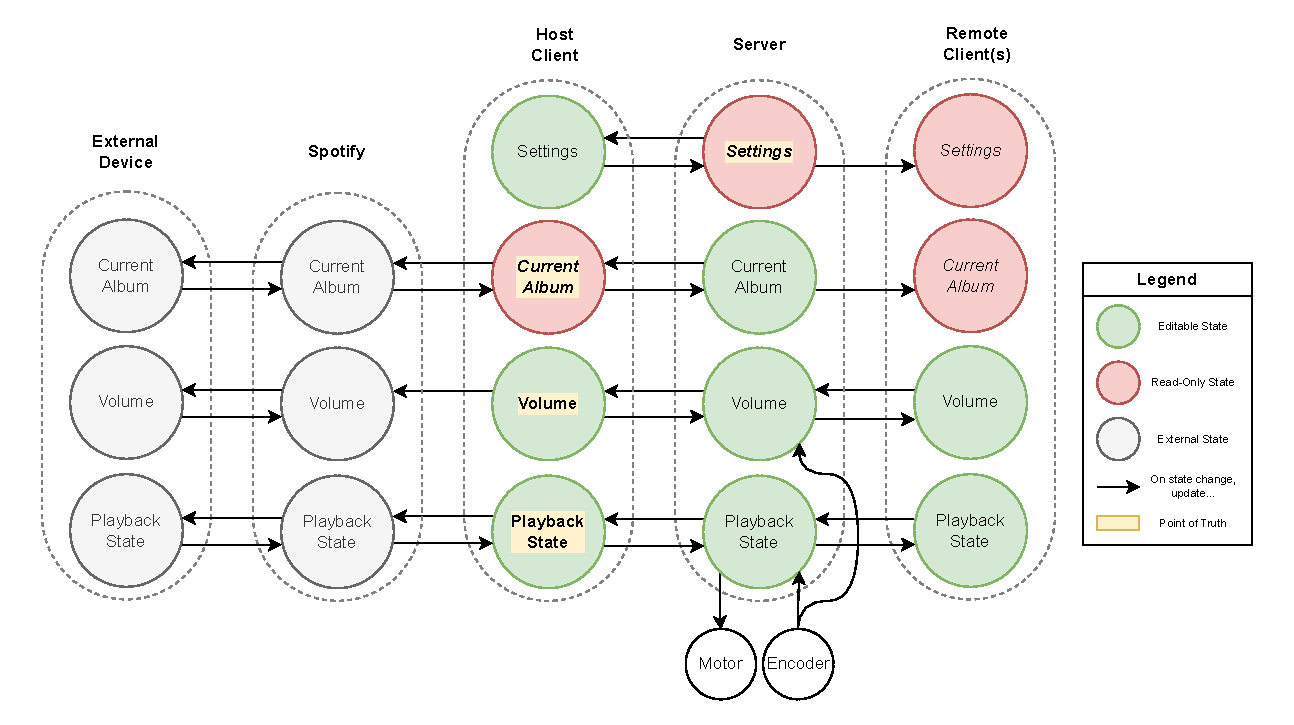
\includegraphics[width=\textwidth]{images/VTT_states.DependencyGraph.pdf}
                \caption{Dependency diagram showing state propagation model between both system and external components, allowing real-time reactivity to state changes from multiple sources.}
                \label{fig:statePropagationDiagram}
            \end{figure}
    
            One complication of this feature, was that there were often superfluous broadcasts. For example, if component A updated component B, then it is wasteful for component B to broadcast that same change back to component A. However, most of these broadcasts were kept, as it essentially created a 'handshake' system where components were not only updating each other, but received confirmation that those updates had been performed. The exception to this was in the front-end clients, where external and internal changes were flagged, to ensure that only internal changes were broadcasted. This was important because React's state system already handles state tracking, and could cause infinite feedback loops, throttling performance and the system's communication bandwidth. Additionally, since the host client interfaced directly with external components, it was best to avoid 'spamming' these components, which could result in timeouts.
    
            \paragraph{Alternate Processes}
    
            Another important aspect was the handling of different triggers for the same processes. For example, how both pressing the physical camera button and uploading an image from a remote device should trigger album detection and playback (see Figure \ref{fig:imageSequenceDiagram}).
    
            \begin{figure}[h]
                \centering
                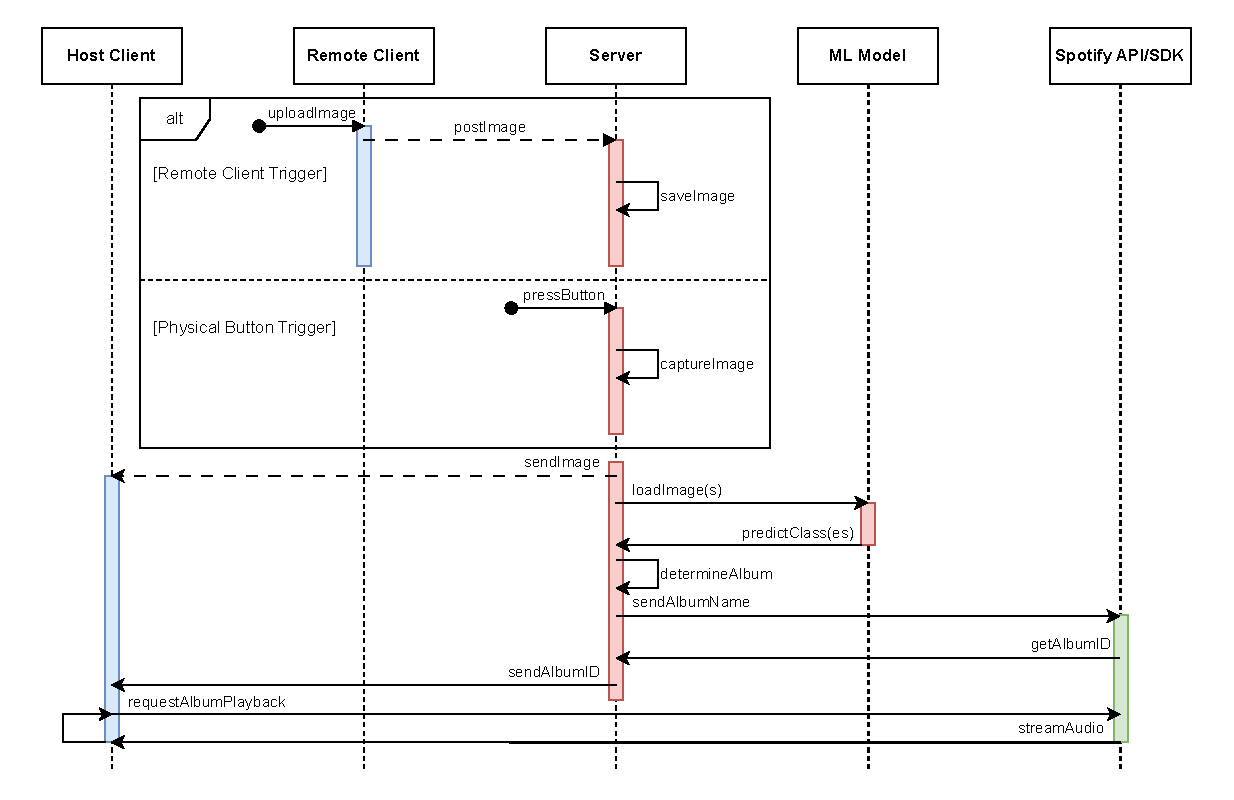
\includegraphics[width=\textwidth]{images/VTT_imageScan.SequenceDiagram.pdf}
                \caption{Sequence diagram showing two alternative triggers (client upload and server capture) leading to image processing and metadata retrieval before sending playback instructions to the host.}
                \label{fig:imageSequenceDiagram}
            \end{figure}
    
            In order to maximise the code's maintainability, re-using the code for the shared part of the process was of utmost importance, however since one trigger was an asynchronous REST endpoint, and the other a low-level polling of hardware. This would have been very difficult to manage if these functions were not in isolated components. Keeping with SRP practices, as decided early on, prior to any development, helped accommodate these mid-implementation changes to the system, with minimal complications.
    
            \subsubsection{Challenges Encountered}
                \begin{temp}
                    1. Change of auth flow, due to 'remote client' introduction
                    2. Removal of barcode detection form spec, due to camera limitations
                    3. \cite{spotify2025security}
                \end{temp}
    
                \paragraph{Authentication handling}
    
                Once the system was changed to allow multiple devices to connect, the whole authentication flow for the server had to be re-written, as it was initially built on the assumption that it would only ever be a single local connection being used. Whilst this required some work, it was a good reminder during the process to challenge the assumptions made during development, and no other changes as large as this had to be made later on in the process, due, at least partially, to this learning experience.
    
                \paragraph{Removal of Barcode Scanning}
    
                It was realised early on that, whilst covers do often have barcodes on their backs, which can uniquely identify the exact album: these barcodes are too low quality to ascertain information from in a image of a full album, without very high quality cameras, which this project did not want to utilise, to avoid reducing the technical accessibility of the system. It could have been setup so that, if a user's scan fails, they can optional re-scan, but this time closer to the image, so that it is just the barcode being captured, but even then, testing found that barcodes are very weak against noise and lighting conditions for general optical cameras (largely due to the fact that they only have one level of redundancy). Some vinyls have QR codes, which are much better suited for general scanning, however, there is no widely adopted system for how a record's QR code correlates to the album (oftentimes it is just a redirect to merch store, etc.). Furthermore, having to position the cover in a specific place, made the system more fiddly than convenient, and so this option was dropped entirely.
    
                \paragraph{Change of Spotify Security Requirements}
    
                In mid-February, towards the end of the development period, when the code was mostly frozen, other than bug-fixes, Spotify announced that it would soon be removing support for HTTP callback URIs, and only allow HTTPS connection, starting on the 9th of April \cite{spotify2025security}. This was problematic for my system, as only utilised HTTP protocols, on the assumption that it was only ever used as a local device (essentially in development mode), rather than as a traditional web-server. As previously mentioned, compliance with API requirements was an important mandate for the project, and this extended to maintaining compliance, too. However, the conversion to HTTPS introduced a fair number of regressions and issues, which took some time to correct, rather late into this phase.
    
                It was an important reminder, that if this sudden change had not been one that could be complied with, then, the agnostic approach of the system would hopefully mitigate the difficulty in switching to another system -- although this would still have been likely to large of a task for this late into the process.
    
        \subsection{Hardware}
    
            To implement the design, the following hardware components were selected:
    
            \begin{itemize}
                \item \textbf{Motor Driver}: TODO
                \item \textbf{Micro Metal Geared motor with Encoder}: 6V 75RPM 210:1
                % https://thepihut.com/products/micro-metal-geared-motor-w-encoder-6v-75rpm-210-1?variant=27740943185&country=GB&currency=GBP&gad_source=1
                \item \textbf{Trust Trino HD webcam}
                % https://dezlwerqy1h00.cloudfront.net/Media/Datasheets/18679-Trust-Trino-Datasheet_en.pdf
                \item \textbf{KY-040 360 Degree Rotary Encoder Module}: 5\,V
                % https://eeshop.unl.edu/pdf/KEYES%20Rotary%20encoder%20module%20KY-040.pdf
                \item \textbf{Standard button}
            \end{itemize}
    
            Additionally, the 'hinge switch' arm was created by simply wiring the Pi to isolated sides of a standard metal hinge, connected to an off-cut piece of wood, shaped similar to an arm.
    
            Figure \ref{fig:circuitDiagram} can be referred to for the configuration of these components with the system.
    
            \begin{figure}
                \centering
                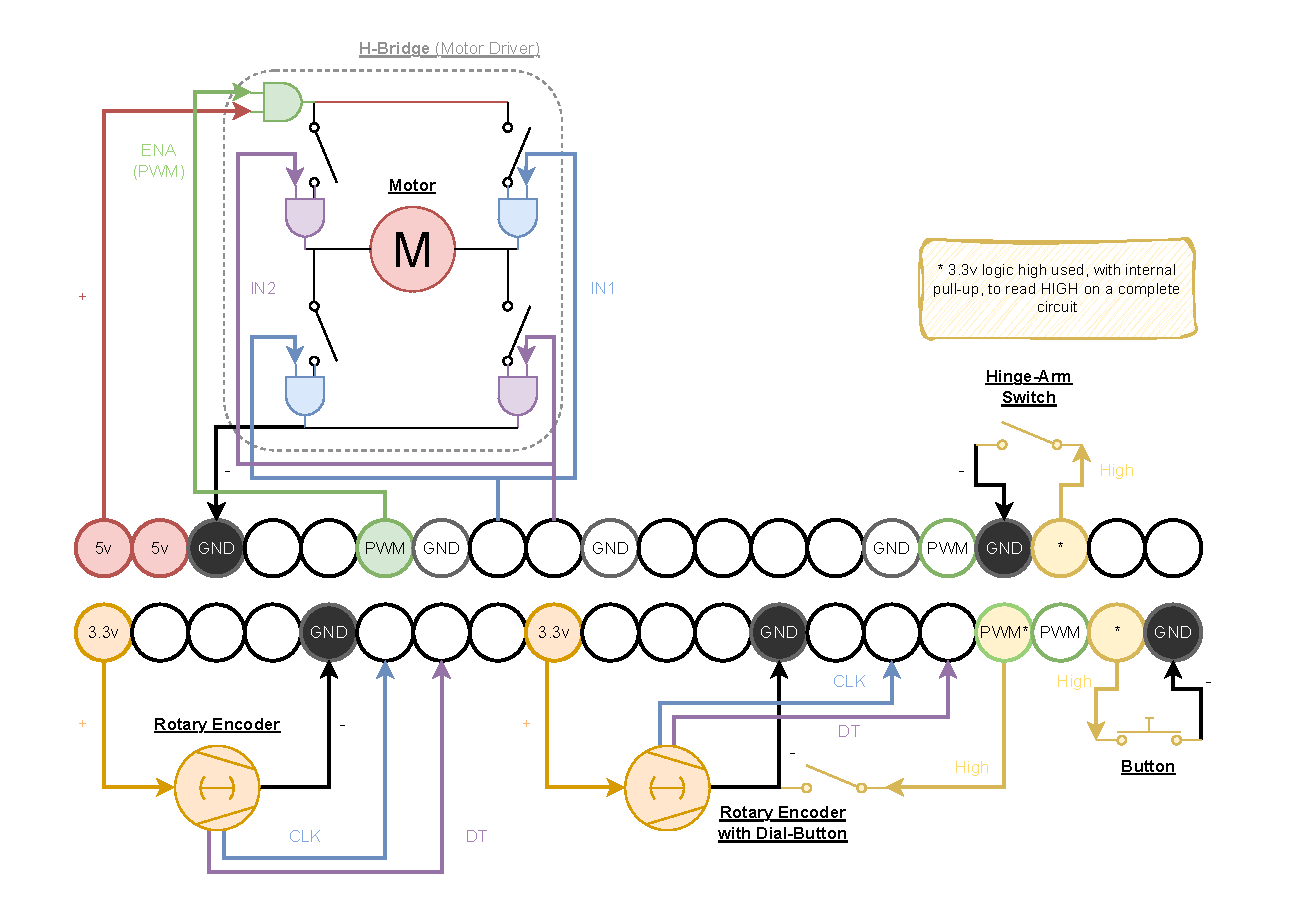
\includegraphics[width=0.5\linewidth]{images/CircuitDiagram.jpg}
                \caption{Circuit diagram of the connected components (TEMP! TODO: FORMALSIE)}
                \label{fig:circuitDiagram}
            \end{figure}
        
            \subsubsection{Challenges Encountered}
    
                During the implementation phase of the project, a few problems were encountered when handling the hardware components.
    
                \paragraph{'Measure Twice, Cut Once'}
    
                    Often, when developing software solution, it is common to use a 'trial and error' approach to make a system work. Whilst development is not a mindless task, developers will often just tweak small changes and run the system until it performs correctly, rather than fully designing every single aspect on paper first. For software, in development environments, this is safe to do and even works well as a time-efficient practice. Many technology stacks even accommodate this, with features such as hot-reloading.
    
                    However, when dealing with hardware, this is not the case. During the development of this product there were a few cases where irreparable damage was done to some components due to the use of the above software debugging technique. Whilst configuring the motor to support PWM, the motor driver's jumper connection (which connected the PWM EN input pin to the 5V pin for constant pulse) had to be removed, to allow the PWM GPIO pin to connect. However, after removing the jumper both pins were exposed, and rather than check which one was the correct pin, a rather careless attitude was taken, just guessing which pin it was. This resulted connecting the 3V PWM GPIO pin to a live 5V current, which fried the GPIO output.
    
                    Thankfully, the damaged pin was one of two which supports PWM on the RPi 5 model, and so, the backup pin was used.
    
                    However, this led to much more caution being used when handling the hardware components afterwards.
    
                \paragraph{Voltage Consumption}
    
                    During early development with the Pi, an unofficial charging cable was used as a power source whilst waiting for the official one to arrive. This cable did not have sufficient wattage for the Pi's specs, and, as a result, it was unable to power the device at high-load without causing the device to turn off.
    
                    To prevent this from being a total blocker, the device was configured to under-clock CPU usage, and some other things, in order to minimise the voltage draw of the device, to minimise how often this would occur.
    
                \paragraph{Overheating}
    
                    Sometimes, during long periods of development, the device would reach very high temperatures. Due to the RPi 5's increased specs over previous models, this is fairly common when running it even for small tasks with only active cooling. This began to throttle performance during long periods of development and/or testing, however, the solution was simply to setup an active cooling solution. Thankfully, the pins for controlling fan PWM based off of CPU temperatures are separate from the standard GPIO pins, and so did not affect any of the other components.
    
      \subsection{Machine Learning Model} \label{sec:mlImp}
    
            For implementation of the ML models, PyTorch was chosen over other libraries (such as TensorFlow, Keras, etc.) due to its superior debugging capabilities and flexibility. Given that this project focused on experimentation rather than production-grade deployment, PyTorch's dynamic computation graph and intuitive design made it a more suitable choice. Experimentation was done through Jupyter notebooks, which aided development due to easily allowing specific code snippets to re-run, and rendering results in-line.
    
            The initial goal was to create a full pipeline that could reasonably run on the Raspberry Pi model. Although, it was known that if the dataset grew beyond a toy sample size, whilst it would be possible to train using the Pi, it would not be efficient. With this in mind, all model training and experimentation was done on desktop computer, utilising an NVIDIA RTX 3060 Ti GPU. Eventually, the idea of running the model on the Pi was dropped entirely, however, it is still technically possible, it is just not reasonable for anything other than very small models (TODO- compare results and training times of RTX vsa Pi).
    
            \subsubsection{Ouroboros Model}
    
                In keeping with the experimental learning-through-development approach, the most basic possible CNN model was initially created, as shown in Figure \ref{fig:BabyOuroboros}. The architecture for this was largely informed by TODO, and the first implementation was referred to as SimpleCNN.
    
                \begin{figure}[htbp]
                    \centering
                    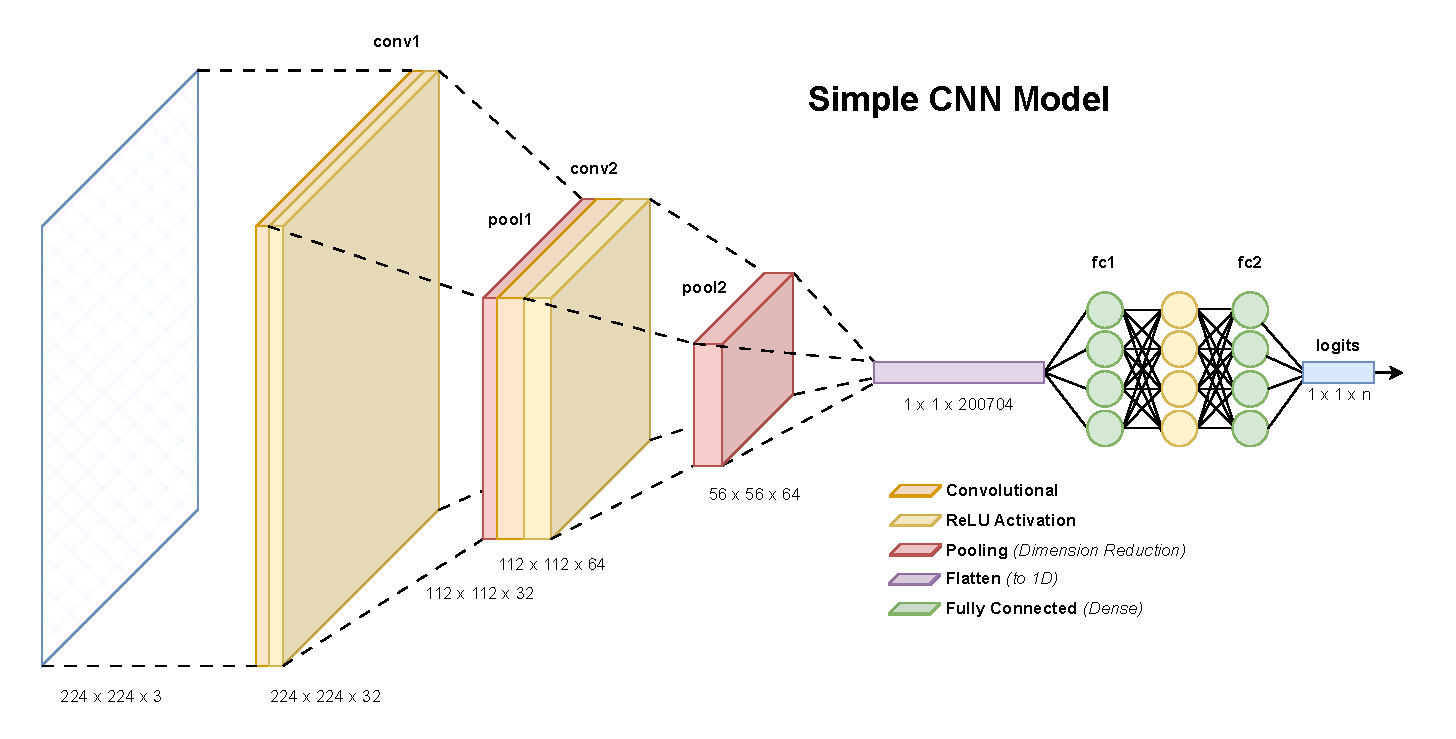
\includegraphics[width=\linewidth]{images/BabyOuroboros.pdf}
                    \caption{Architecture for simple CNN model}
                    \label{fig:BabyOuroboros}
                \end{figure}
    
                The first iteration of this model (SimpleCNN 'Mini') was trained on only the exceptionally small TODO dataset, as a proof of concept. Figure \ref{fig:SimpleCNN-Mini_Train} shows how the models accuracy increased as training progressed. Whilst the model rather quickly converged and showed good results on the training data (eventually overfitting), the validation dataset's accuracy did climb in slow intervals, but never exceeded 60\%. Whilst this was a good start, it was thought that the problem with this poor generalisation likely came from the sheer small scale of the dataset.
    
                All input data was normalised according to the some dataset statistic:
                    \[
                    x' = \frac{x - \mu}{\sigma}
                    \]
    
                Initially, this was calculated as a channel-wide measure of the full combined dataset. However, the standardised ImageNet distribution was also used, with \( \mu = [0.485, 0.456, 0.406] \) and \( \sigma = [0.229, 0.224, 0.225] \). Figure \ref{fig:normalisedArts} shows an example batch of images, normalised to the ImageNet standard.
        
                \begin{figure}[h]
                    \centering
                    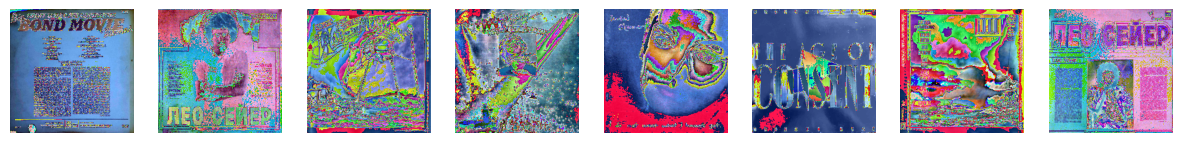
\includegraphics[width=\textwidth]{images/NormalisedArts.png}
                    \caption{Example of normalised dataset batch.}
                    \label{fig:normalisedArts}
                    \caption*{
                        Original artworks are © their respective copyright owners
                        \footnotesize These images have been processed for research/educational purposes and do not intend to infringe upon the original copyrights.
                    }
                \end{figure}
    
                Conforming the data to an external distribution can be a good practice for consistency and compatibility, particularly if there was a chance of later using transfer learning or pre-trained models.
    
    
                \begin{figure}[h]
                    \centering
                    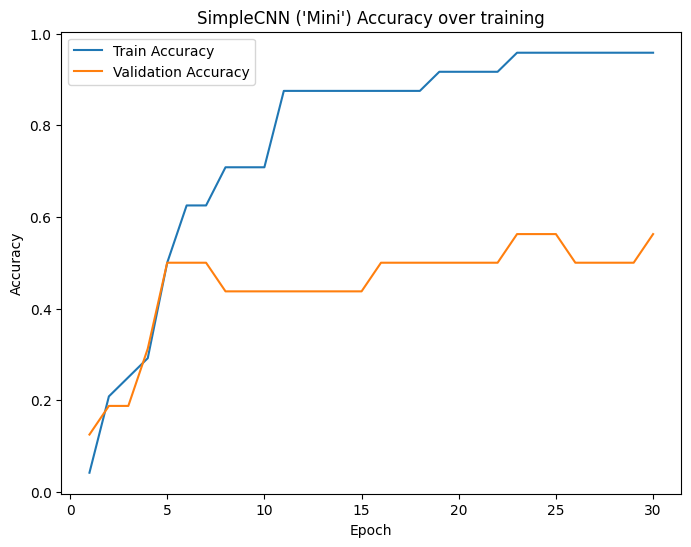
\includegraphics[width=\textwidth]{images/SimpleCNN-Mini_Train.png}
                    \caption{TODO}
                    \label{fig:SimpleCNN-Mini_Train}
                    \caption*{Higher is better. Training of a SimpleCNN model on \ref{data:mini}; validated against \ref{data:val}.}
                \end{figure}
    
                The same model architecture was then used to train on a much a larger dataset (TODO). However, this model performed horrendously with the sudden increase of data. As shown in Figure \ref{fig:SimpleCNNs_TrainLoss-Mini_Train} whilst the loss (distance of predictions from the true results) decreases rather smoothly on the smaller dataset, when trying to learn from TODO, the model very sharply overfits, and actually worsened in validation performance, never even improving beyond the smaller dataset's initial performance. Figure \ref{fig:SimpleCNNs_PeakAccuracy-Mini_Train} shows the differences of the best-observed performances of this model architecture across these two training scenarios, showing that performance decreased as the dataset increased.
        
                \begin{figure}[h]
                    \centering
                    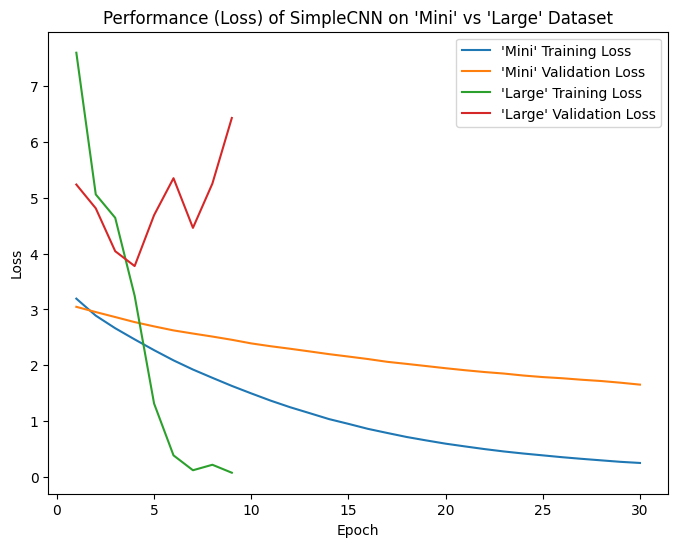
\includegraphics[width=\textwidth]{images/SimpleCNNs_TrainLoss.png}
                    \caption{Comparison of SimpleCNN architecture performance on different sized datasets}
                    \label{fig:SimpleCNNs_TrainLoss-Mini_Train}
                    \caption*{Lower is better. Trained on 'Mini' (\ref{data:mini}) and 'Large' (\ref{data:large}) datasets; both validated against \ref{data:val}.}
                \end{figure}
        
                \begin{figure}[h]
                    \centering
                    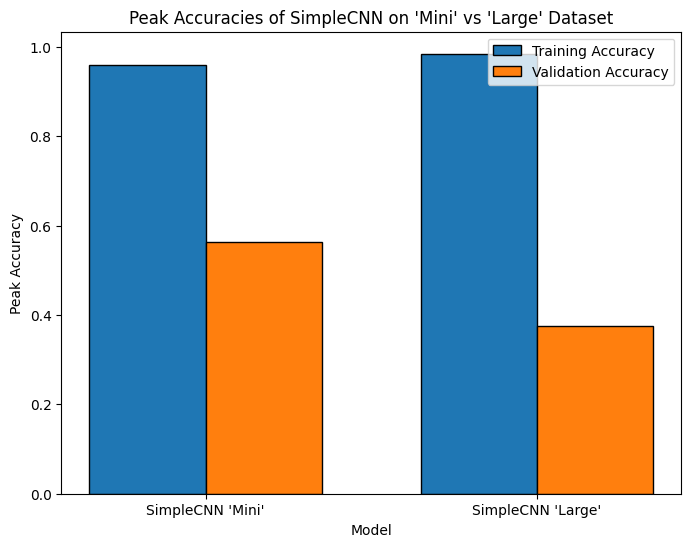
\includegraphics[width=\textwidth]{images/SimpleCNNs_PeakAccuracy.png}
                    \caption{Comparison of best-case SimpleCNN performance on different sized datasets}
                    \label{fig:SimpleCNNs_PeakAccuracy-Mini_Train}
                    \caption*{Trained on 'Mini' (\ref{data:mini}) and 'Large' (\ref{data:large}) datasets; both validated against \ref{data:val}.}
                \end{figure}
    
                This model performed reasonably on small datasets, but could not scale, and so was labelled as Baby Ouroboros.
    
                In order to improve the results for the large dataset, a deeper model would be required. Various experiments were done with various configurations and depths of model (broadly named DeepCNN), however, as the range of albums had increased, even with a greater depth, the feature extraction mechanisms seemed to be lacking. As networks become deeper they require exponentially more data in order to learn sufficiently.
    
                After the results of the deeper versions of Baby Ouroboros did not prove very fruitful, a new architecture was planned. Rather than trying to train a model from scratch, it was decided to trial using a feature-extractor from an existing model, which had been trained on a much larger and more generalised dataset. In order to do this, the ResNet18 model selected, which has been trained on the immense ImageNet library. In theory, a custom solution could have still been trained using this publicly available dataset, with the published parameters and architecture of these models, however, for faster development iterations, it was decided to use a pre-trained feature-extractor, and to either fine-tune it, or just build a classifier system on top of it.
    
                The ResNet18 model, by itself has a powerful feature extractor, however just appending a classifier head on top would yield purely random results, if not further refined through specialised training for the album-recognition task.
    
                \subsubsection{Model Experiments}
    
                    Initially, the ResNet18 model's weights were frozen entirely, with only the append 'classifier head' being tuned. This was done to ensure that no heavy biasing or loss of previously learnt information occurred. This approach yielder better results than the in-house DeepCNN model, immediately. However, additional experiments were also run with unfreezing and fine-tuning different aspects and combinations of the base model, to further improve performance.
        
                    \paragraph{Model Hyperparamaterisation}
        
                        A large-scale hyper-parameter grid search was conducted, training the model over various different combinations of value for certain aspects: learning rate, weight decay, number on unfrozen layers, batch size, etc. The results of one test, evaluating different learning rates and weight decays, over each training cycle (epoch), can been seen in Figure \ref{fig:ResNet_AugGrid}, with the best observed accuracies shown in Figure \ref{fig:ResNet_AugGridHist}.
                
                        \begin{figure}[h]
                            \centering
                            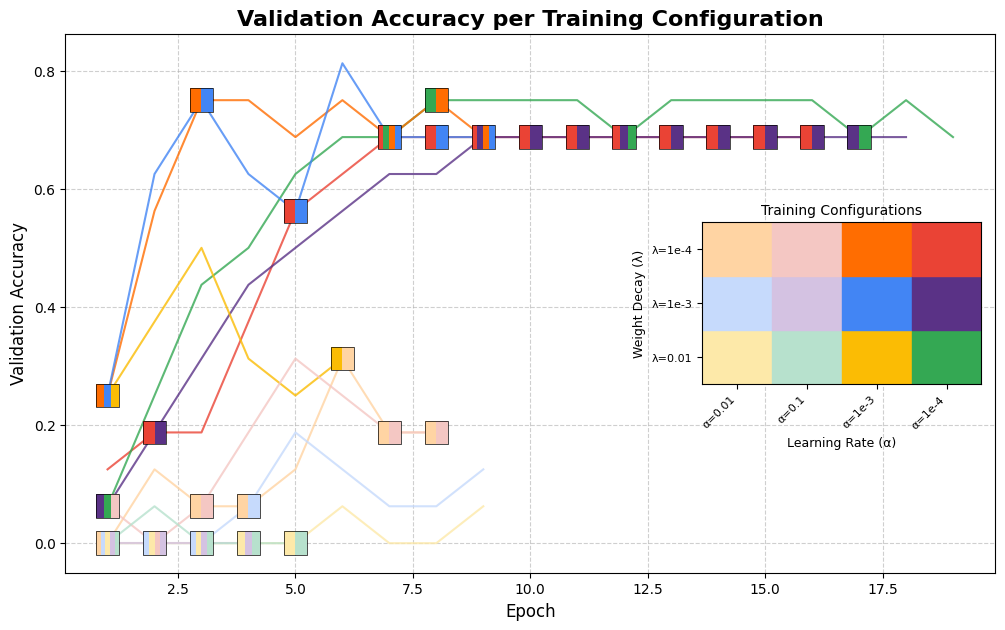
\includegraphics[width=\textwidth]{images/ResNetCNN_AugGrid.png}
                            \caption{Performance results of ResNet18 fine-tuned model hyperparamter grid search}
                            \caption*{Performed on \ref{data:aug} training set (1,176 images) with batch size of 8; validated against \ref{data:val}. Early stopping used when validation loss degraded, so not all configurations ran for equal epochs. Where multiple configurations have the same performance at the same epoch, a square marker indicates which colours are represented.}
                            \label{fig:ResNet_AugGrid}
                        \end{figure}
                
                        \begin{figure}[h]
                            \centering
                            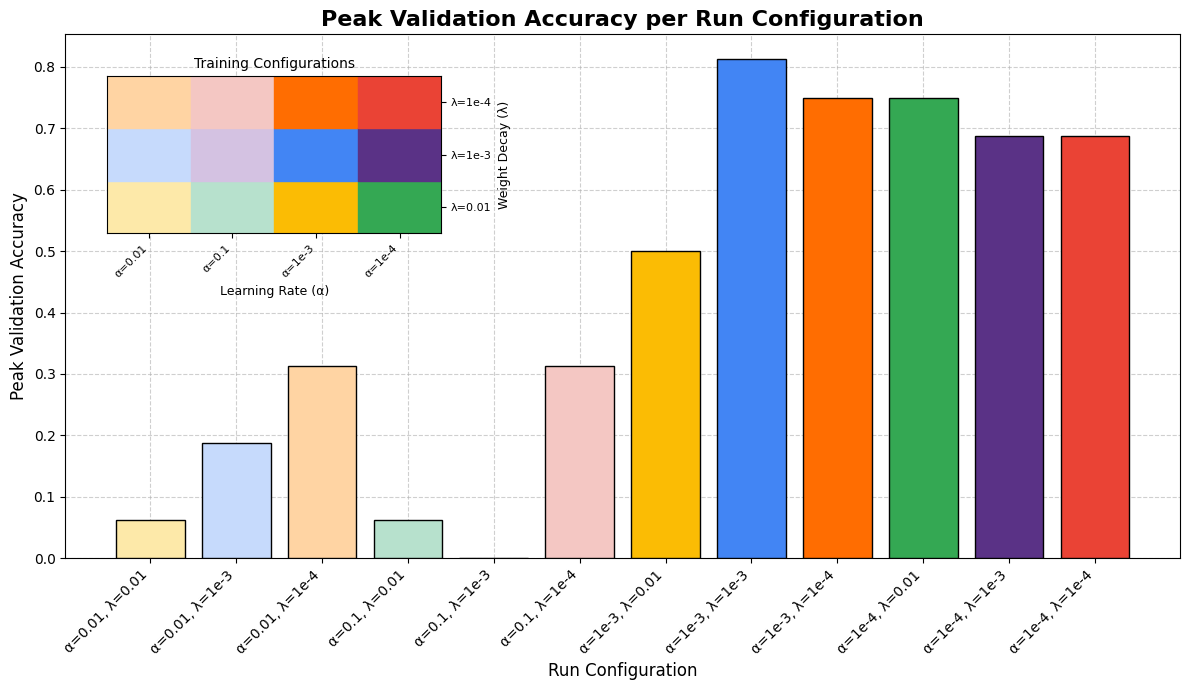
\includegraphics[width=\textwidth]{images/ResNetCNN_AugGridHist.png}
                            \caption{Best-case performance results of ResNet18 fine-tuned model hyperparamter grid search}
                            \caption*{
                                Full set of accuracies during training can be seen in Figure \ref{fig:ResNet_AugGrid}.
                            }
                            \label{fig:ResNet_AugGridHist}
                        \end{figure}
        
                    \paragraph{Data Augmentation}
        
                        In addition to experimenting with the model's configuration, the data was also investigated. Since the design phase, it was known that this model would likely not need much generalisation techniques, due to being a closed-world task, however, to make the model as robust as possible, data augmentation was still investigated. In a real use case, even though the images will be very similar to their training data, there could be slight fluctuations in rotation, size, and lighting or fading of the artwork. Additionally, some extreme transformations might occur, such as the artwork being fully upside down. In order to make the system handle this, each epoch of training was bolstered with augmented copies of with artificial transformations, de-colourings, and cropping taking place (see Figure \ref{fig:augmentedArts} for an example).
    
                        \begin{figure}[h]
                            \centering
                            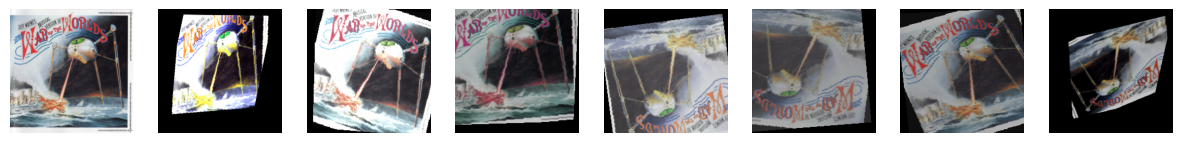
\includegraphics[width=\textwidth]{images/AugmentedArts.png}
                            \caption{Example of augmented dataset batch (without normalisation).}
                            \label{fig:augmentedArts}
                            \caption*{
                                The first image is the unaltered original, whereas the rest of the batch have all be augmented over their rotation, size, cropping, colour, affinity and perspective.
                            }
                            \caption*{
                                Original artworks are © their respective copyright owners
                                \footnotesize These images have been processed for research/educational purposes and do not intend to infringe upon the original copyrights.
                            }
                        \end{figure}
    
                        This augmentation was generated 'on-the-fly' during training, meaning no modified image was saved or stored beyond the training epoch. Additionally, this meant that each epoch had slightly different variations it was learning on. This made the training process better for generalisation, serving as a forced dropout of seen images; however, the training process became slower, requiring more training epochs to accurately learn from the data, as well as the dataset now be scaled to be a factor bigger, increasing the time taken to train.
    
                        Even with GPU optimisation, as the dataset multiplied in size, it became to hold to store within the available VRAM at once, and so batch sizes had to be decreased from ~32 to ~8, in most cases, further slowing the training process.
    
                        This 'on-the-fly' approach also had drawbacks, as it required additional rendering computations in every epoch cycle, however, the performance gains made the extra time taken a worthwhile trade-off.
        
                    \paragraph{Data Hyperparamaterisation}
    
                        Not only was the model configuration rigorously tested under various alterations, but also the training dataset.
    
                        One notable requirement of a CNN model, is that all input data must be the same size, that is, the images must all be of uniform dimensions. The initial baseline used was 244x244, however it was theorised that greater fidelity versions of images could improve quality.
    
                        As per Figure \ref{fig:CNNSize_Perf}, various image sizes were tested in the TODO model, to varying degrees of observed success. Whilst the 124x124 size did have the highest peak in performance, the 244x244 was most consisent in its performance. The more extreme sizes seemed to perform most poorly, likely due to the smallest images having too great of a loss in details to be learnable, whereas the larger images were likely subject to too much noise and variation, as well as potentially requiring more epochs or a deeper network with larger convolution kernels to adequately learn details.
            
                        \begin{figure}[h]
                            \centering
                            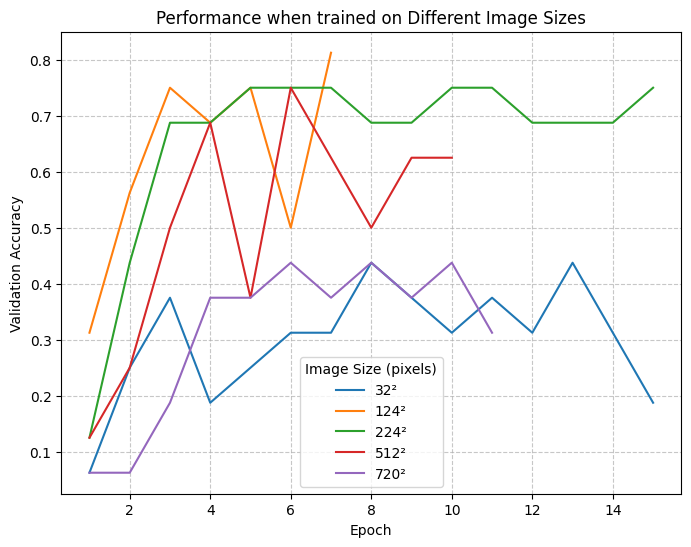
\includegraphics[width=\textwidth]{images/CNNSize_Perf.png}
                            \caption{TODO}
                            \label{fig:CNNSize_Perf}
                            \caption*{Results are averaged over multiple attempts.}
                        \end{figure}
    
                        The 124x124, 244x244, and 512x512 configurations were further experimented with, however, as per Figure \ref{fig:CNNSize_Time}, training time scaled roughly quadratically as the area of the image increased, an expected result seeing as convolution is highly dependent on per-pixel processes (even when done in batches, via matrix representations). For this reason, 244x244 was selected as the primary image size, due to having the most consistent performance with very small time constraints compared to the smaller 124x124 form factor.
    
                        Additionally, when switching to utilise the ResNet feature extractor, the 244x244 was especially the best-performing, as this was the input size used for the model's initial training.
                
                        \begin{figure}[h]
                            \centering
                            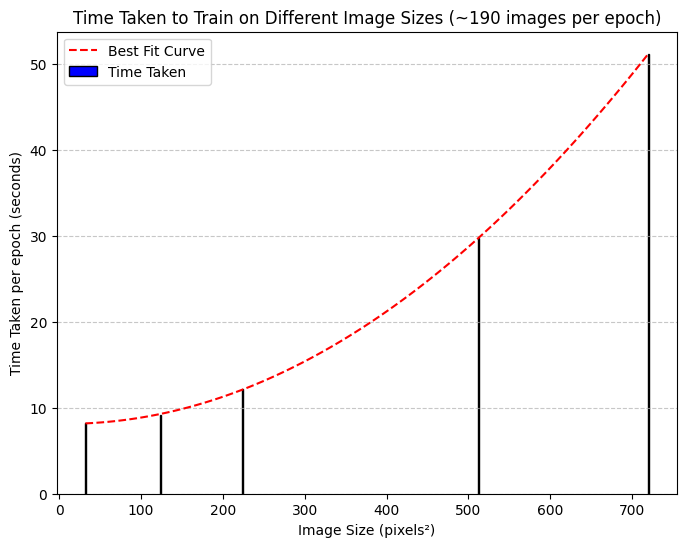
\includegraphics[width=\textwidth]{images/CNNSize_Time.png}
                            \caption{TODO}
                            \label{fig:CNNSize_Time}
                            \caption*{Results are averaged over multiple attempts.}
                        \end{figure}
    
            \subsubsection{Amphisbaena Model}
    
                The Ouroboros model, using the ResNet18 architecture, was additionally built upon to have two classification heads, allowing the model to learn different categories for the same items. In addition to learning the album, this allowed learning a de-coupled artist value. Using a single network, diverging into two output heads at the end allowed for shared learning from feature extraction, and reduced redundant duplication of resource-heavy processes (for example, this task could be done with two fully separate models, but would double the training time).
    
                \begin{temp}
                    Multi-Head Model Diagram
                \end{temp}
    
                This was largely done as an experimental feature, as it was unknown how well an artist can be detected, on unseen data, from other albums of the same artist. Whilst author classification is an area being explored for visual artists, this is a much more generalised task for album covers, as two albums by the same musician may feature two drastically different artworks produced by different artists, with little-to-no overlap. However, some musicians do have stylistic consistency in their albums covers. A notable example in pop culture is Ed Sheeran, whose albums often feature mathematical symbols and paint effects (see Appendix \ref{app:Cult}, Figure \ref{fig:EdMeme} for a comedic example). Additionally, albums by the same musician may consistently feature a logo, brand, or even the their likeness, which could be enough information for a deep model to learn from. And, finally, many album arts are done by the same artist for a single performer or band, and so even stylistic aspects could still be beneficial.
    
                \begin{figure}[h]
                    \centering
                    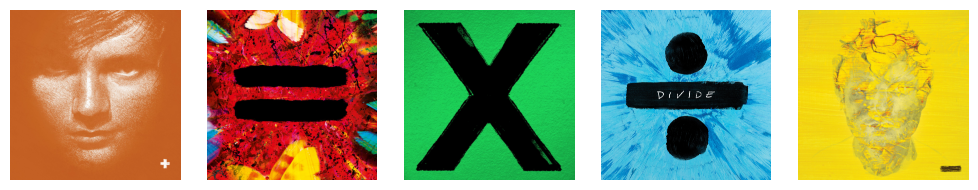
\includegraphics[width=0.6\textwidth]{images/EdAlbums.png}
                    \caption{Album covers of Ed Sheeran’s studio albums}
                    \label{fig:EdAlbums}
                    \caption*{+ (2011), = (2021), × (2014), ÷ (2017), and − (2023). \\ Images © Asylum Records / Atlantic Records. Retrieved from Cover Art Archive.}
                \end{figure}
    
                After some experimentation, it was found that the model was able to achieve some level of success. As a proof of concept, as part of the TODO dataset, four of Ed Sheeran's albums were included. These images (the first four, from the left, in Figure \ref{fig:EdAlbums}) were able to learn enough information such that the − (2023) album (right-most image) was able to be correctly identified as an Ed Sheeran album (64\% confidence).
    
                It is worth noting that this use case is a particularly ideal one, however, with Ed Sheeran's album all being very uniformly consistent.
    
                The aim to experiment with additional channels as classification, such as genre of decade, was ultimately not viable within the time, alongside the rest of development, and so were left.
                
    
            \subsubsection{Hydra Model}
    
                The creation of the dynamically-expandable classification system was conducted, however, due to time constraints only minimal experimentation was conducted. The use-case for this model was that, if a user had a large collection and had set up this system to classify them, but then bought a new record, they would have to fully re-train a new model from scratch, to accommodate the new addition. Furthermore, if the model was performing poorly on some albums, the user would, theoretically, be able to inform the system of this, essentially acting as a manual annotator, which could be used to give higher weightings to these albums, to tune the model to match user expectations. This goal of high-level model customisation was challenging, however.
    
                At first, the idea was to simply fine-tune the previously trained models, using a new collection of data. However, it was quickly found that catastrophic data loss occurred when altering weights without the original training images to validate them.
    
                In order to avoid the retention or re-downloading of copyrighted images to be required for this system to work, instead a matrix database was created. The classification model essentially has two components: a feature extractor and a classifier. The idea was to, once initial training was complete, run each training image through the feature-extractor only, and to store the numerical tensor (the embedding) in this database. Then, if a future revision of the model was desired, the feature extractor could be frozen, then classifier could be re-initialised to allow an additional album, and the already-extracted features could be fed directly into the classifier, alongside the new data going through the full model, to ensure training saw both sets of data.
    
                Whilst this technique showed better results, it was still prone to catastrophic data loss, either biasing towards the new data, or the original data. Freezing the feature extractor, whilst allowing to remember old features better, prevented the model from being able to correctly learn new albums; however, removing this constraint resulted in the previously extracted data sometimes being almost-random in accuracy-- sometimes performing okay, but other times not; with no consistent way of ensuring ideal performance.
    
                For this, a PNN architecture was created, allowing a dynamic number of heads to operate in parallel, using a weighted consensus approach to generate a single classification. This idea still utilised a single, frozen feature extractor, utilising the retained embeddings, however, rather than replacing the classifier, a new classifier was added in tandem to the original one. Then, during training, the two heads were weighted, through cross-entropy loss, so that the final result was the 'consensus' of the two. Essentially, the original model was preferred, unless the second model had a high degree of confidence that it was a new class, in which case, the system delegated to the newer head if, and only if, the original head was not also highly confident.
    
                This system showed promising improvement over the early attempts, however performance degradation was still significant, with the model dropping from \~80\% confidence on the initial images to \~30\% (though, accuracy was maintained in the very small testing sample set used). This showed that the dynamic approach was at least, potentially,  viable for a full-scale solution. However, due to time constraints, no further experimentation was done on this concept.
    
                A major issue with the initial vision, however, was that if a user wanted to update their model, this training system would ideally need to be run on-demand on the Pi. Due to the need of the vector database, and a deep model, for the results acquired, this means that the training process would be significantly slow, on the SBC, and therefore, might have to be done as a once-per-day system, as a limitation of the hardware.
    
            \subsubsection{Documentation}
    
                Additionally, in order to make the models clear and distinct from one another, as well as being potentially useful to other developers, a model card \cite{Mitchell_2019} was created, for each.
            
            \subsubsection{Challenges Encountered}
    
                On the 8th of October 2024, the Internet Archive experienced a significant cyberattack that led to a temporary outage of its services, including the Cover Art Archive. The breach exposed data from approximately 31 million user accounts, revealing email addresses, screen names, and bcrypt-hashed passwords. %https://www.forbes.com/sites/larsdaniel/2024/10/20/internet-archive-breached-again-third-cyber-attack-in-october-2024/
    
                This posed a fairly significant issue for the project, as the Cover Art Archive had been selected as the source of the training datasets, however, as a joint project between the Internet Archive and MusicBrainz, was among the affected services. Users reported issues accessing cover art images during the outage. %https://community.metabrainz.org/t/internet-archive-down-possibly-hacked/718418
    
                This outage lasted for weeks, with components being brought back online one-by-one,
                %https://blog.archive.org/2024/10/21/internet-archive-services-update-2024-10-21/
                with the Cover Art Archive not being restored until after the 21st. Fortunately, a small 'toy' scale dataset had already been accumulated, in addition to the physically-owned copies that could be used, and so this did not become too much of an issue for the project. Whilst model training was limited to small-scale models, these weeks were used mostly on development of the web components.
    
                If, however, this outage had continued for longer, then serious consideration of finding a new service would have been required. During these weeks, additional research into such systems was done, an Last.fm was selected as a backup. But, once the Cover Art Archive was restored, no further issues occurred during development, regarding data availability. Although, more outages of the service have been reported, post-development. % https://hackread.com/internet-archive-archive-org-down-power-outage/
    
    %%%%%%%%%%%%%%%%%% SECTION 5 %%%%%%%%%%%%%%%%%%
    \section{Results} % edit section heading as appropriate
        \begin{temp}
            What was actually produced?
        \end{temp}
        % results of soft/hardware testing
        % screenshots of UI / program output
        \subsection{Software Artefact}
    
            \begin{figure}[h]
                \centering
                \begin{minipage}[b]{0.45\textwidth}
                    \centering
                    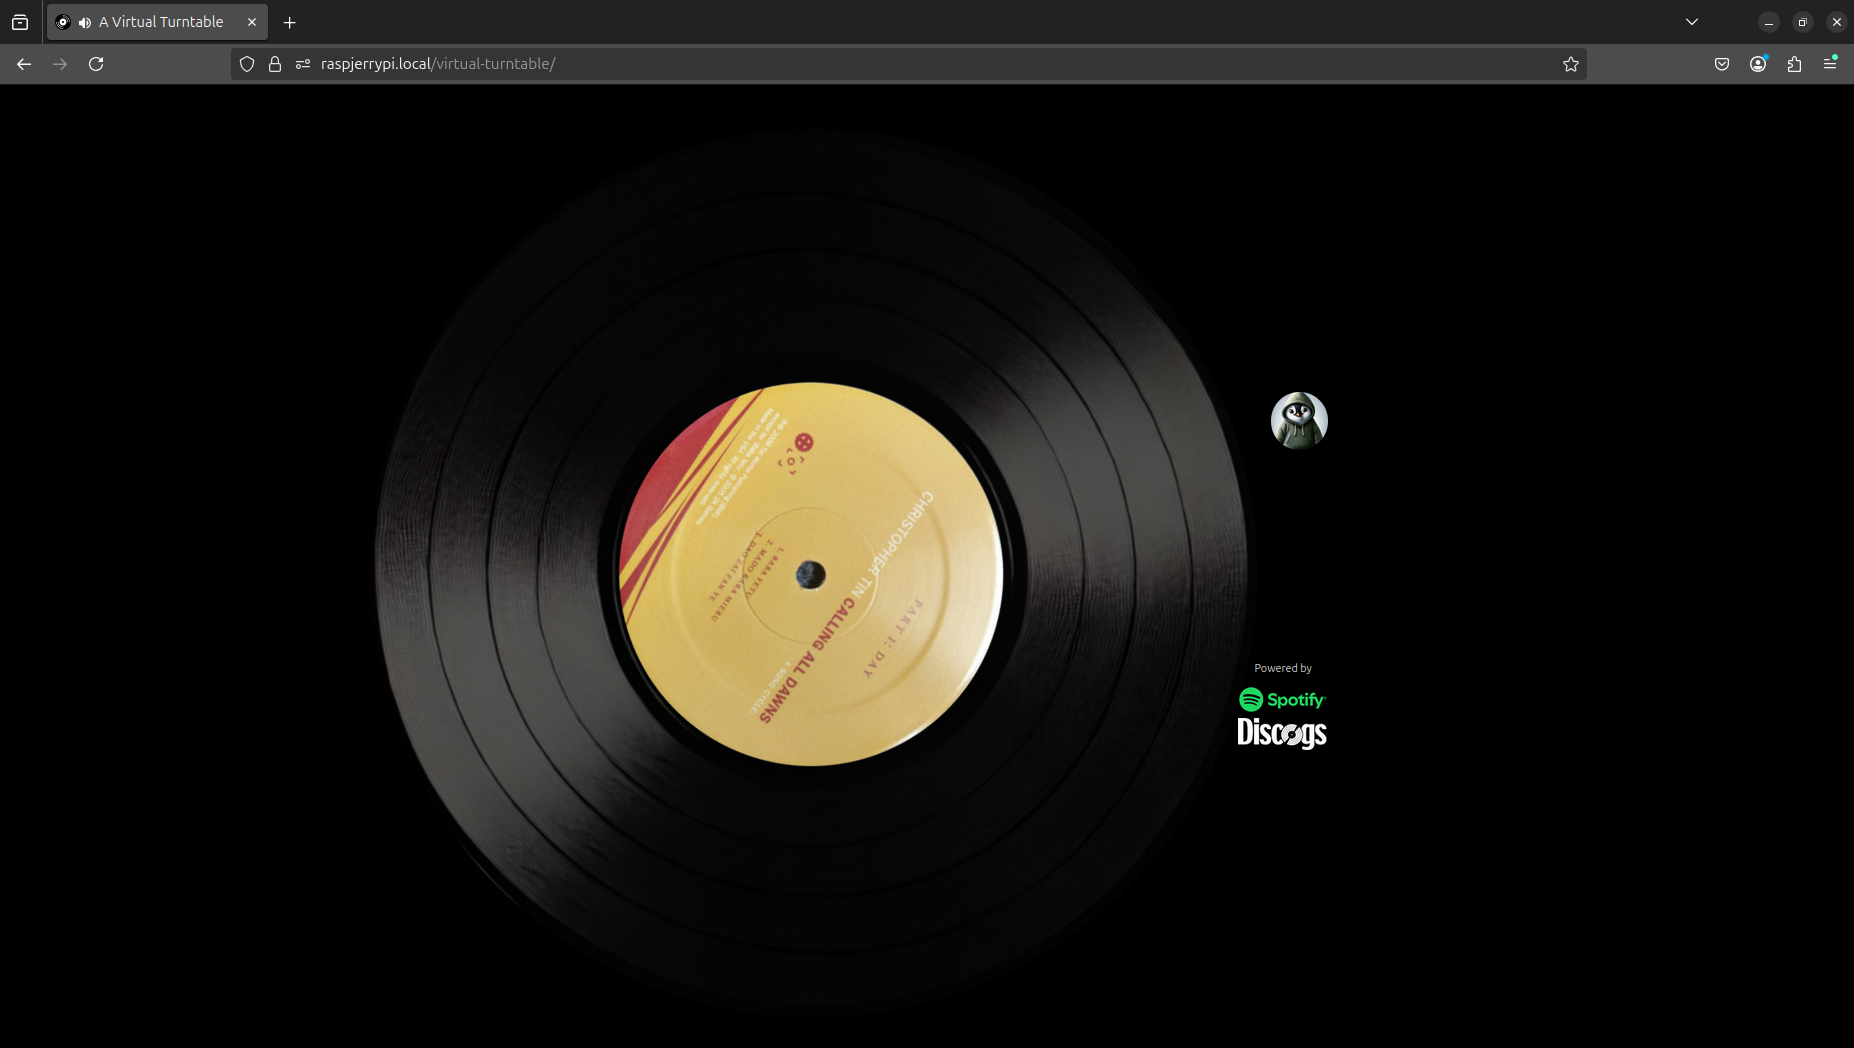
\includegraphics[width=\textwidth]{images/screenshots/HOST_Quiet.png}
                    \caption{Host client playing a track}
                    \label{fig:hostQuiet}
                \end{minipage}
                \hfill
                \begin{minipage}[b]{0.45\textwidth}
                    \centering
                    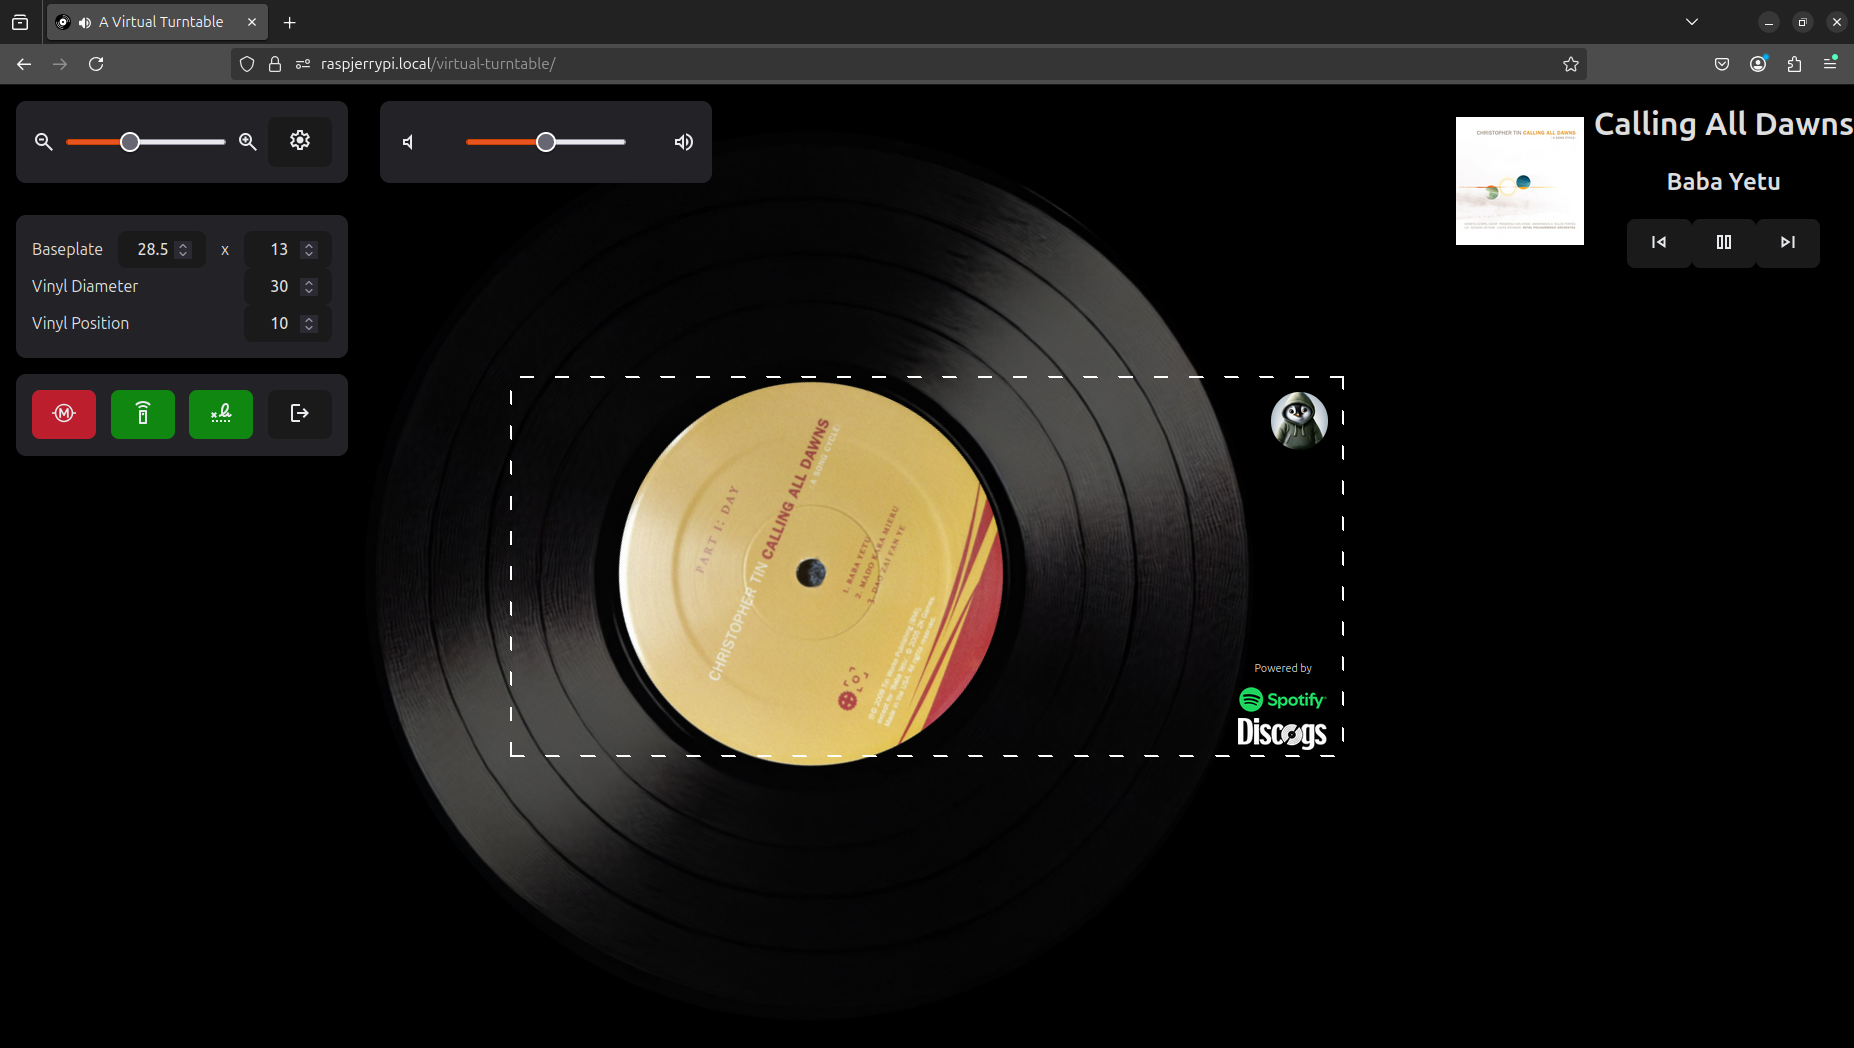
\includegraphics[width=\textwidth]{images/screenshots/HOST_GUI.png}
                    \caption{Host client playing a track, with UI overlays}
                    \label{fig:hostGui}
                \end{minipage}
            \end{figure}
            
            \begin{figure}[h]
                \centering
                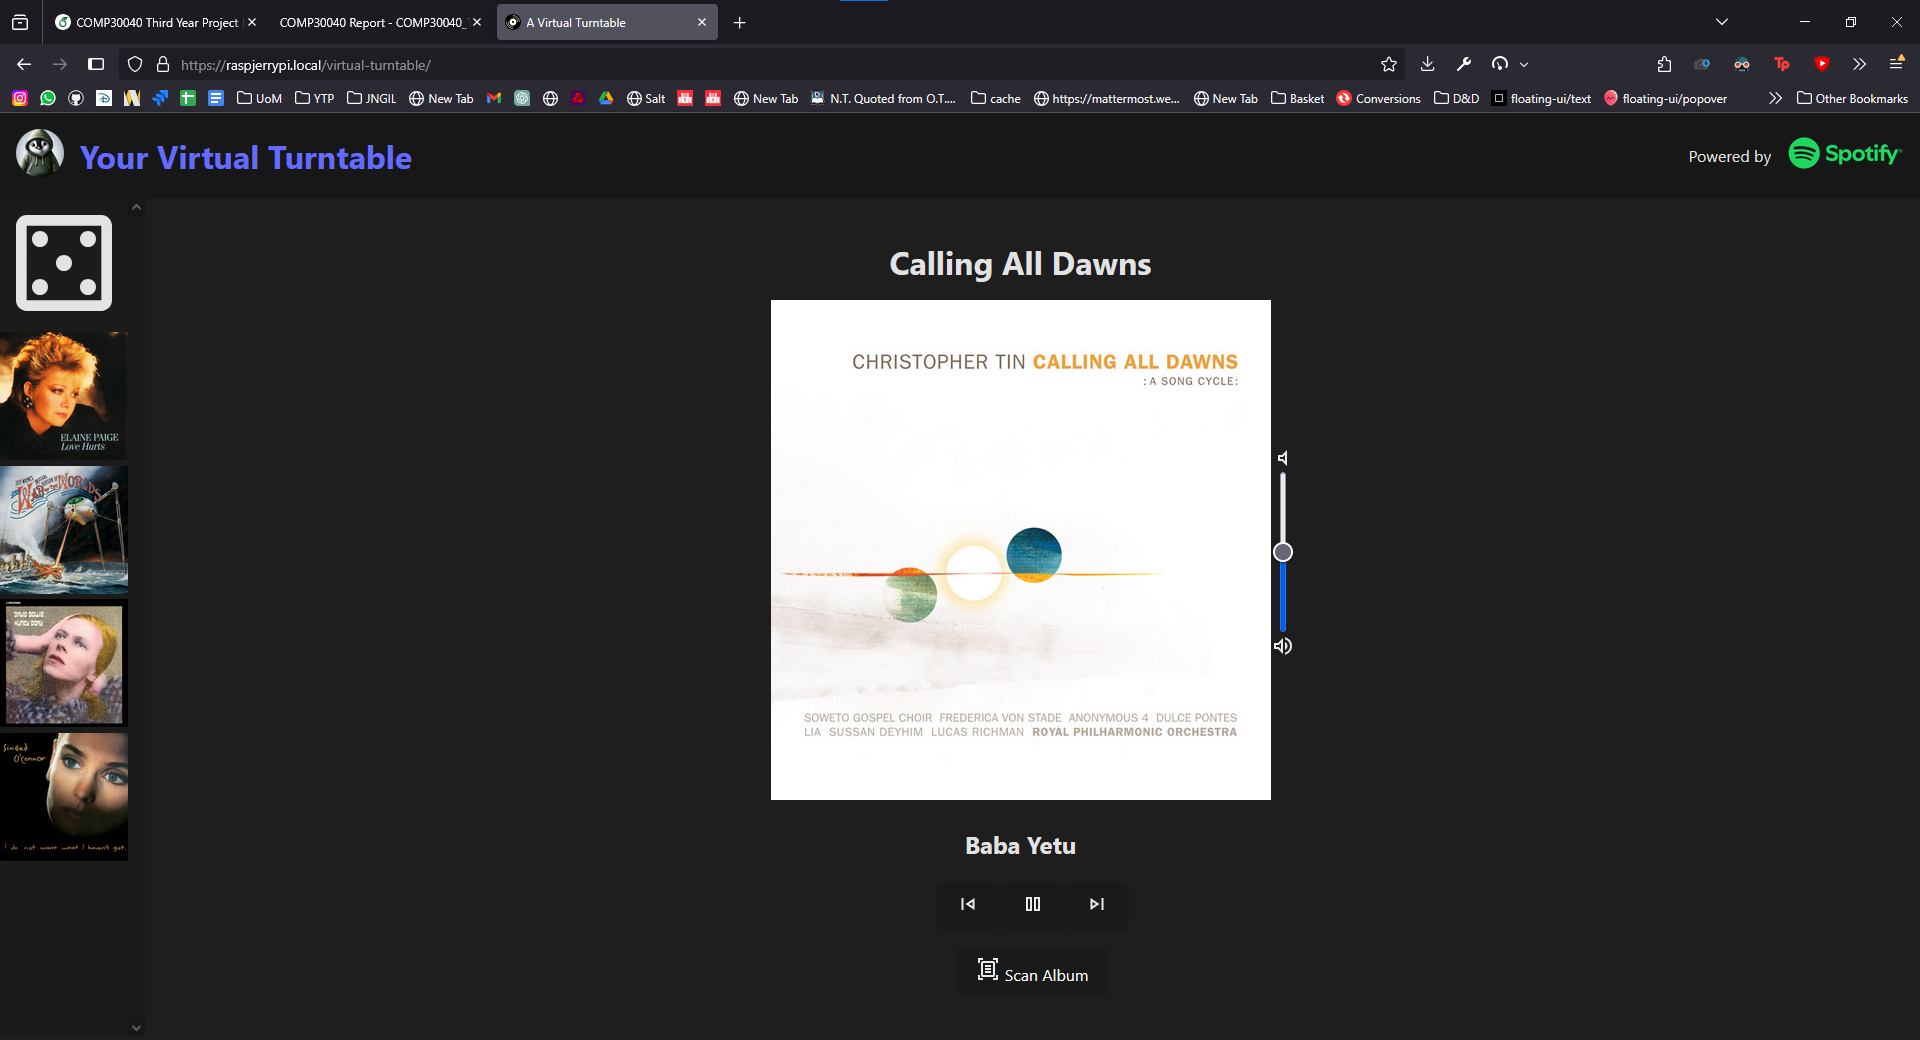
\includegraphics[width=0.4\textwidth]{images/screenshots/LAPTOP.png}
                \caption{Screenshot of a remote client (PC) connected to the host}
                \label{fig:laptop}
            \end{figure}
            
            \begin{figure}[h]
                \centering
                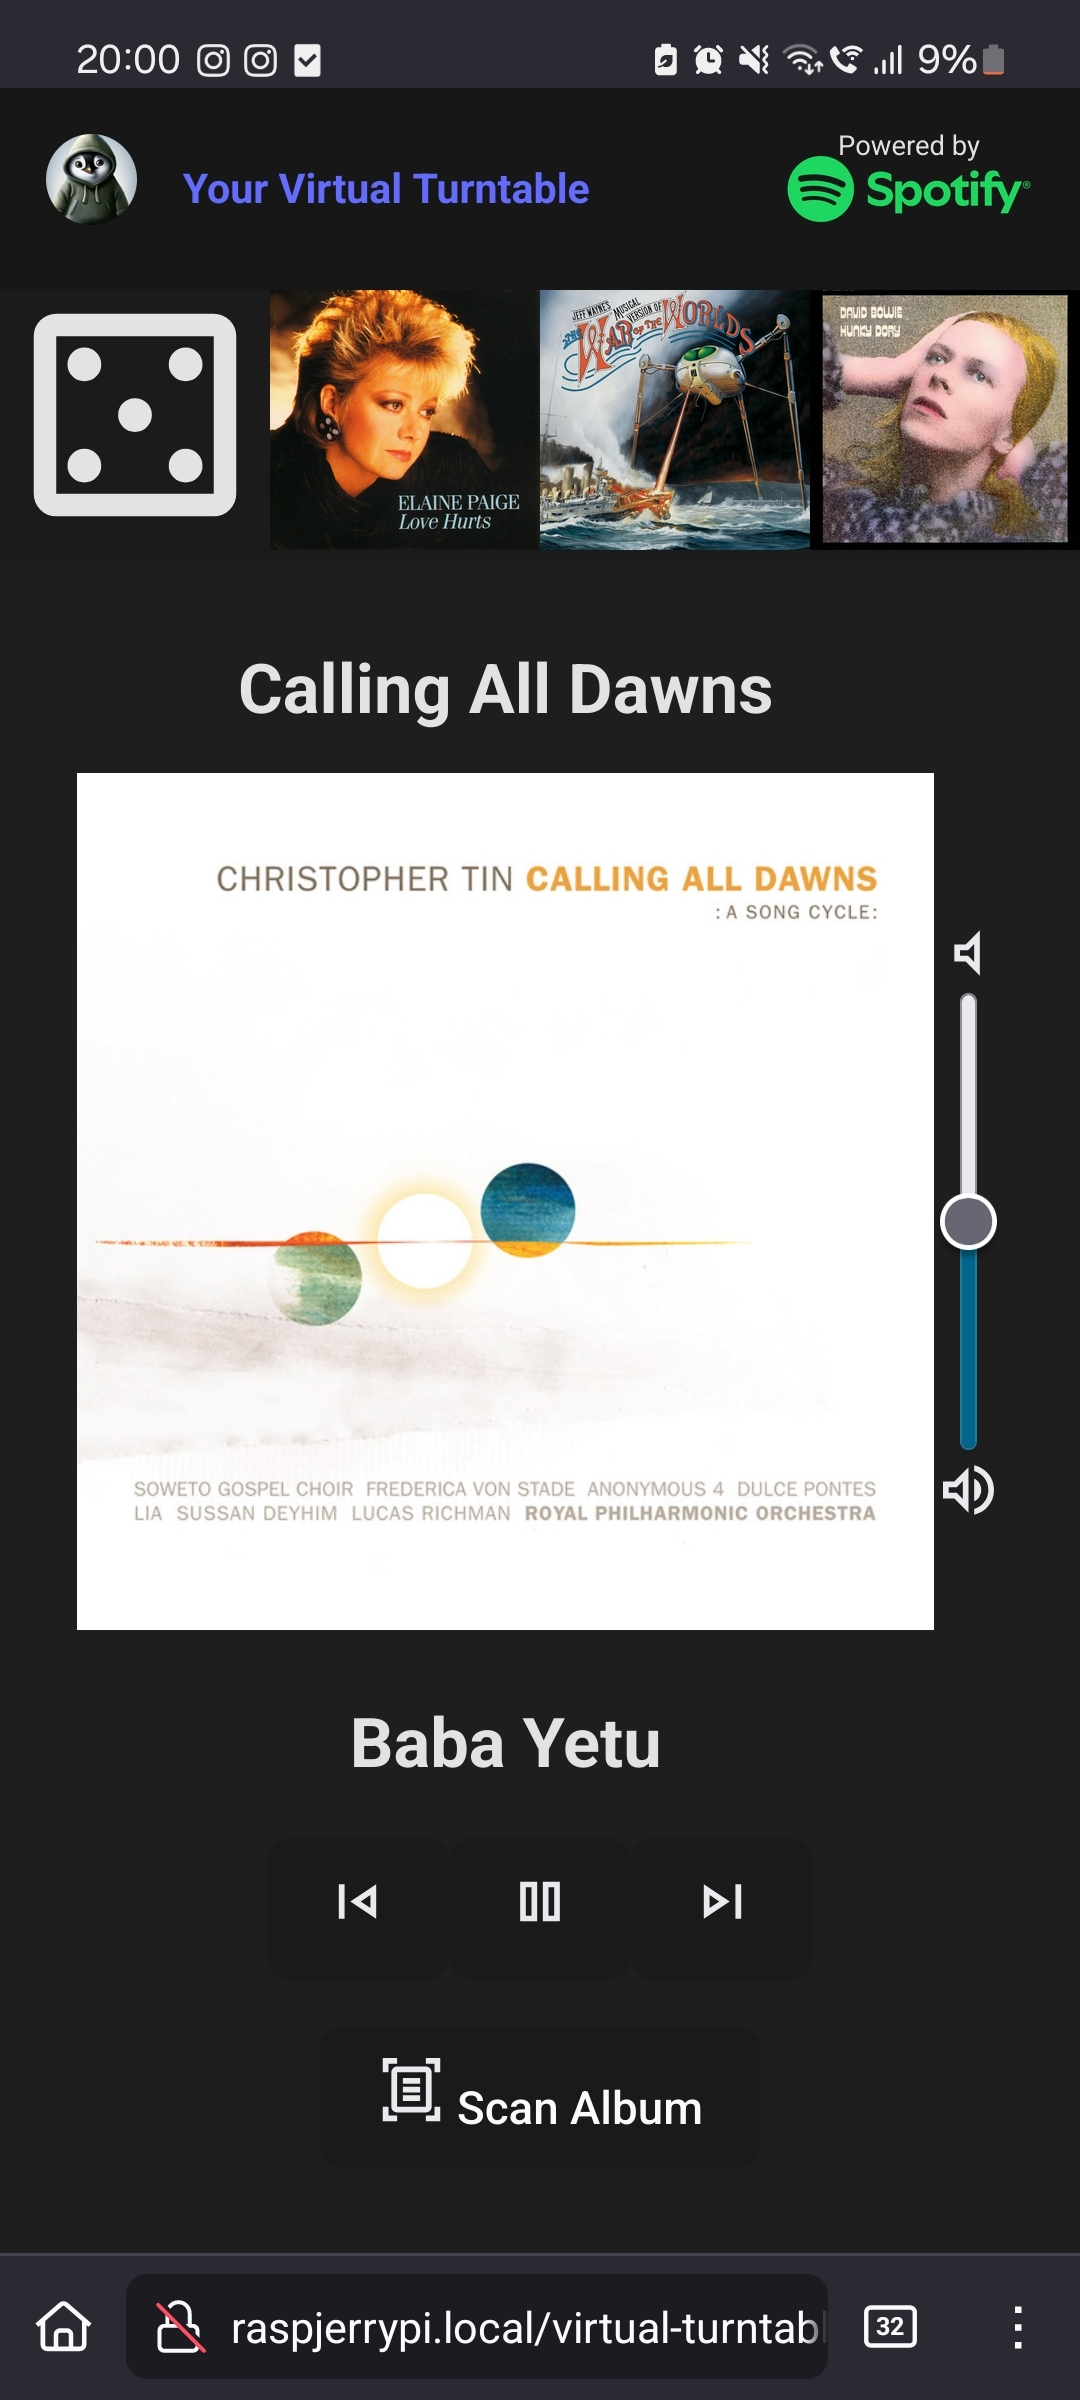
\includegraphics[width=0.4\textwidth]{images/screenshots/PHONE.jpg}
                \caption{Screenshot of a remote client (mobile) connected to the host}
                \label{fig:phone}
            \end{figure}
        
        \subsection{Hardware Artefact}
    
            \begin{figure}
                \centering
                \includegraphics[width=0.5\linewidth]{images/SystemInUse.jpg}
                \caption{Photograph of the system (scanning an album)}
                \label{fig:SystemInUse}
                \caption*{"Held Together By Prayers and Duck Tape" TODO: TEMP!}
            \end{figure}
    
            \begin{figure}
                \centering
                \includegraphics[width=0.5\linewidth]{images/SystemBirdsEye.jpg}
                \caption{Photograph of the system (top-down)}
                \label{fig:SystemTopDown}
                \caption*{"Held Together By Prayers and Duck Tape" TODO: TEMP!}
            \end{figure}
    
    %%%%%%%%%%%%%%%%%% SECTION 6 %%%%%%%%%%%%%%%%%%
    \section{Evaluation}
        % does it do what it is supposed to do?
        % how well?
        % how well against others?
    
        This section evaluates the system’s functionality and performance across several key criteria.
        
        \subsection{Quantitative Evaluation}
    
            \subsubsection{Album Classification Accuracy}
    
                To assess classification accuracy, the model was trained on the full dataset and evaluated on a held-out test set of 34 images. It achieved a top-1 accuracy of 91.18\%, correctly predicting 31 out of 34 albums. Of the three errors, two were due to the model being trained on visually distinct variant covers (see Figure \ref{fig:ModelEval}), with only one test image matching the training version. If these variant covers are treated as anomalies, the accuracy rises to 97.05\%. While the test set is relatively small and not exhaustive, it reflects a reasonable physical collection a user might own.
    
                \begin{figure}
                    \centering
                    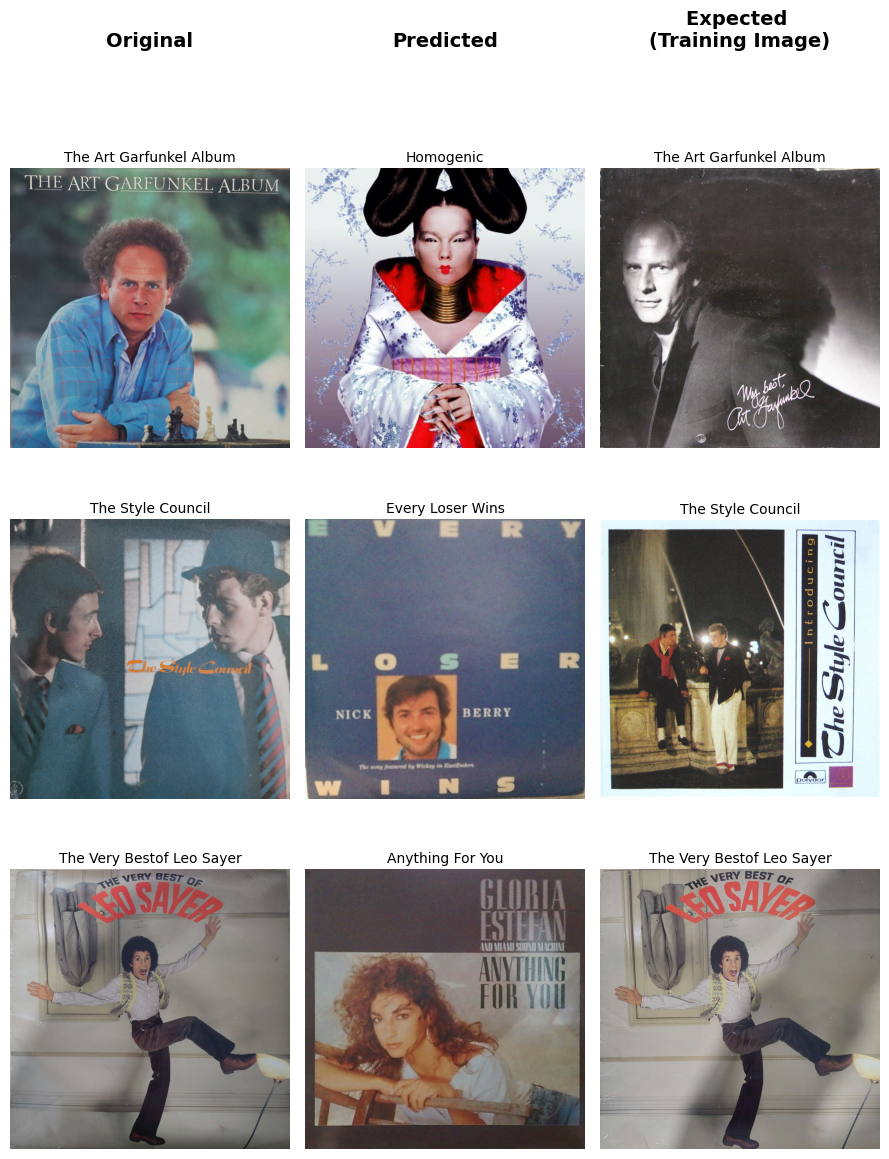
\includegraphics[width=0.5\linewidth]{images/modelEval.png}
                    \caption{Examples of misclassifications from the validation set}
                    \caption*{
                        Each row shows a failure case: the original input image (left), the model’s incorrect prediction (centre), and the correct training image (right). Errors primarily occured due to cover variants.
                    }
                    \caption*{
                        Artworks are © their respective copyright owners.
                    }
                    \label{fig:ModelEval}
                \end{figure}
    
            \subsubsection{Metadata Retrieval Accuracy}
    
                Since metadata retrieval depends on external sources and network responses, evaluation was performed manually. A representative set of 32 albums was tested using automated centre-level retrieval. Of these, 4 were exact matches, 8 were correct but returned variant covers (e.g., CD editions), 2 matched the correct artist but wrong album, 15 returned no label, 2 returned unrelated images, and 1 returned an entirely incorrect label. In addition to the centre label, the Spotify album is also selected, which affects the textual metadata and album cover shown on remote devices. Of these same albums, 3 albums were compilations not present on Spotify, which led to retrievals of other compilations with similar themes (e.g., disco, Bond themes, Christmas). One album was a musical, correctly identified by title but with different performers, and one “best of” album was not available on Spotify, but yielded the correct artist. Despite some gaps, most queries retrieved results that were either correct or thematically relevant. With only a fairly low percentage of fetching bad data from Spotify (84.38\%; up to 96.88\% excluding compilations) the primary metadata source is correct, and as this only failed for particularly niche albums, a more standard collection should be very robust in the system.
    
                The centre label system was less reliable, yielding a relevant result only 43.75\% of the time, with a correct label only 37.5\%; however, as this only serves additional supplementary data, this is an acceptably low success rate. Particularly as a user could add their own image samples to the system's cache directory, fixing this problem. However, future improvements to this pipeline would certainly be beneficial.
    
    
            \subsubsection{System Responsiveness}
    
                Responsiveness was measured by timing the interval between user input (e.g., cover upload or classification trigger) and result delivery. The system was treated as an end-to-end pipeline. Tests across varying devices and network conditions showed average response times of under 2 seconds for classification and under 4 seconds for metadata retrieval, using the Ouroboros model trained on the full dataset. Worst-case latency occurred on slower connections, reaching up to 7 seconds. Overall, the system remained responsive and usable across typical usage scenarios.
    
            \subsubsection{Code Robustness}
    
                The codebase was evaluated through a suite of automated unit tests, covering core components such as image processing, metadata retrieval, and classification logic. The overall test pass rate is reported, and code coverage was estimated to ensure critical paths are exercised. No critical failures or regressions were observed during testing.
    
                The frontend achieved an average of 71.5\% statement coverage, with particularly strong performance in components like WebSocketManager.ts (96\%) and SpotifyPlayer.ts (92.4\%). The backend reached 66.2\% average coverage across core Python modules, with several key files such as sessionManager.py, stateManager.py, and modelHandler.py reaching very high coverages of 89–100\%. However, some components — notably main.py, routes.py, and training utilities — remain untested due to their hardware dependence or being out of scope.
                
                Overall, the combined project-wide coverage stands at 71.5\%, reflecting a strong foundation with room for expanding test coverage to the integration and hardware layers.
    
        \subsection{Qualitative Evaluation}
        
            \subsubsection{User Experience -- Usability}
    
            \subsubsection{User Experience -- Aesthetics}
            
        \subsection{Comparative Analysis}
            \begin{temp}
                Comparison with Existing Systems
            \end{temp}
    
        \subsection{Limitations and Trade-offs}
    
        \subsection{Ethical Implications}
            \begin{temp}
                What is the impact of the finished product?
            \end{temp}
    
    %%%%%%%%%%%%%%%%%% SECTION 7 %%%%%%%%%%%%%%%%%%
    \section{Conclusions and future work} % edit section heading as appropriate
        \subsection{Conclusions}
          % summarise results
          % achieved aims?
          % improvements!
        
        \subsection{Future work}
          % ideas for further work
          % big ideas; what could be done with my project?
    
    %TC:ignore
    %%%%%%%%%%%%%%%%%% REFERENCES %%%%%%%%%%%%%%%%%%
    %\clearpage % uncomment to start on a new page if wanted
    \printbibliography[title={References},heading=bibintoc] % a single list of references for the whole thesis
    
    
    
    %%%%%%%%%%%%%%%%%% APPENDICES %%%%%%%%%%%%%%%%%%
    \begin{uomappendix} 
        % screen dumps of UI
        % important but large results
        \section{Project outline}
    
            \begin{temp}
                Project outline is a required appendix. Put here.
            \end{temp}
            
            % Vinyl is back! According to the \href{https://www.nme.com/news/music/uk-vinyl-sales-2023-reach-highest-level-since-1990-3563676}{NME}, UK sales of vinyl in 2023 were the highest seen since 1990. Vinyl has always remained popular among niche genres, but we are also seeing mainstream artists like Taylor Swift and Lana Del Rey releasing and selling large volumes of albums on the format. Vinyl records have also recently been added into the ONS "Basket of Goods and Services": a carefully selected set of items representative of the goods and services that UK consumers typically spend their money on (\href{https://www.ons.gov.uk/news/news/arecordrevivalthatscookingupastormvinylmusicandairfryersspintheirwayintothebasketofgoods}{ONS}).
            
            % Fans of the format claim better sound reproduction, with a fuller frequency range and a "warmth" lacking in digital formats such as CD. Playing vinyl requires specialist equipment: while the ritual of putting a disc on the turntable and dropping the needle is, for some, part of the experience, it can also be seen as an inconvenience.
            
            % The aim of this project will be to develop an application that supports a blending of the physical and digital worlds. A physical artefact such as an LP is scanned using a camera. The information on the label or cover is then used to identify the release which can be played. This content could be retrieved from a streaming service such as Spotify or Apple Music, an artist site such as \href{https://bandcamp.com/}{Bandcamp}, or the user's own personal media library. This would then allow a user to "play" their records without a turntable. Although the audio quality may not match that of vinyl, such an application would appeal to those who like to collect vinyl for its own sake, or who appreciate the larger format artwork that comes with an old school LP. The application could run on a mobile phone or specialist hardware such as a Raspberry Pi equipped with a camera.
            
            % Example methods that could be used for identification of the release include barcodes, QR codes or OCR acting on label text.
            
            % For a stretch goal, the application could be extended to cover other media: the cassette tape (\href{https://www.theguardian.com/music/2023/apr/20/fun-way-consume-music-why-sales-of-cassette-tapes-soaring}{Guardian}) is also experiencing a comeback, although the \href{https://en.wikipedia.org/wiki/8-track_cartridge}{eight-track} is unlikely to be retrieved from the dustbin of history.
            
            % The project should be considered as challenging. It will require integration of several technologies and some creativity.
        
        \section{Risk assessment}
            \begin{temp}
                Risk assessment is a required appendix. Put here.
            \end{temp}
    
        \section{Model Cards}
            \begin{temp}
                TODO
            \end{temp}
    
        \section{Datasets}
    
            \subsection{Training Set 'Mini'} \label{data:mini}
    
                15 albums; 24 data points
    
            \subsection{Training Set 'Large'} \label{data:large}
    
                \ref{data:mini}
                
                + 68 classes; + 133 data points (a_dig)
    
                + 20 classes; + 39 data points (b_phys)
    
            \subsection{Training Set Augmented} \label{data:aug}
    
                \ref{data:large} * 6
    
            \subsection{Validation Set} \label{data:val}
    
                14 albums; 16 data points
    
            \subsection{Test Set} \label{data:test}
    
                \ref{data:val} + 1 class (\_null); + 20 data points
    
        \section{Evaluation Results}
    
            \subsection{Unit Tests}
                \paragraph{Front End (Vitest)}
                \begin{verbatim}
    -----------------------|---------|----------|---------|---------|
    File                   | % Stmts | % Branch | % Funcs | % Lines |
    -----------------------|---------|----------|---------|---------|
    All files              |    71.5 |    81.81 |   58.71 |    71.5 |
     src                   |   76.76 |    82.08 |   47.27 |   76.76 |
      App.tsx              |   58.64 |    90.24 |   33.33 |   58.64 |
      RemoteController.tsx |   77.91 |    82.85 |      30 |   77.91 |
      VirtualTurntable.tsx |   84.65 |     75.9 |   40.74 |   84.65 |
      WebSocketManager.ts  |      96 |      100 |    90.9 |      96 |
      root.tsx             |       0 |        0 |       0 |       0 |
     src/APIs              |    42.1 |      100 |      60 |    42.1 |
      IMusicAPI.ts         |       0 |        0 |       0 |       0 |
      IMusicPlayer.ts      |    42.1 |      100 |      50 |    42.1 |
     src/APIs/Local        |       3 |        0 |       0 |       3 |
      LocalPlayer.ts       |       3 |        0 |       0 |       3 |
     src/APIs/Spotify      |   76.47 |    94.11 |   72.72 |   76.47 |
      SpotifyAPI.ts        |    66.4 |    92.85 |   66.66 |    66.4 |
      SpotifyPlayer.ts     |    92.4 |       95 |   76.92 |    92.4 |
     src/common            |   72.05 |    66.66 |   70.83 |   72.05 |
      Dialogue.tsx         |    56.6 |     62.5 |   66.66 |    56.6 |
      Tooltip.tsx          |   79.25 |    46.15 |    62.5 |   79.25 |
      WebcamCapture.tsx    |   78.78 |    86.66 |      80 |   78.78 |
     src/types             |     100 |      100 |     100 |     100 |
      Music.ts             |       0 |        0 |       0 |       0 |
      vendor.ts            |     100 |      100 |     100 |     100 |
     src/utils             |     100 |      100 |     100 |     100 |
      blob.ts              |     100 |      100 |     100 |     100 |
    -----------------------|---------|----------|---------|---------|
                \end{verbatim}
    
                \paragraph{Back End (Pytest)}
                \begin{verbatim}
    Name                                          Stmts   Miss  Cover
    -----------------------------------------------------------------
    app\APIs\DiscogsAPI.py                           49      2    96%
    app\APIs\MusicAPI\IMusicAPI.py                   47     13    72%
    app\APIs\MusicAPI\SpotifyAPI.py                 132     61    54%
    app\enums\StateKeys.py                           16      0   100%
    app\main.py                                     182    182     0%
    app\modules\Hardware\IHardwareController.py      31      9    71%
    app\modules\Hardware\piController.py            149    130    13% 
    app\modules\centreLabelHandler.py                70     11    84% 
    app\modules\modelHandler.py                      70      7    90%
    app\modules\sessionManager.py                    48      0   100%
    app\modules\stateManager.py                      35      4    89%
    app\modules\websocketHandler.py                  55     43    22%
    app\routes.py                                   161    161     0%
    app\utils.py                                     35      8    77%
    modelling\__init__.py                             0      0   100%
    modelling\getAlbumArt.py                        131    131     0%
    modelling\models\Amphisbaena.py                 127    109    14%
    modelling\models\BabyOuroboros.py                22     14    36%
    modelling\models\Ouroboros.py                   107     89    17%
    modelling\models\__init__.py                      0      0   100%
    modelling\models\train.py                        87     87     0%
    modelling\models\utils\CustomDataset.py         100     80    20%
    modelling\models\utils\ModelType.py               5      0   100%
    modelling\models\utils\RandomFlip.py             12      4    67%
    modelling\models\utils\Transforms.py              4      0   100%
    modelling\models\utils\__init__.py                0      0   100%
    -----------------------------------------------------------------
                \end{verbatim}
    
            \subsection{System Evaluation}
                \paragraph{Ouroboros Model}
                \begin{verbatim}
    Evaluation Results:
    Total images evaluated: 34
    Correct predictions: 31
    Accuracy: 91.18%
    
    Failures:
    TheArtGarfunkelAlbum_ArtGarfunkel_1984 --> Homogenic_Björk_1997
    TheStyleCouncil_TheStyleCouncil_1983 --> EveryLoserWins_NickBerry_1986
    TheVeryBestofLeoSayer_LeoSayer_1979 --> AnythingForYou_GloriaEstefanandMiamiSoundMachine_1988
                \end{verbatim}
    
        \section{Image Overflow}
    
            \begin{figure}[h]
                \centering
                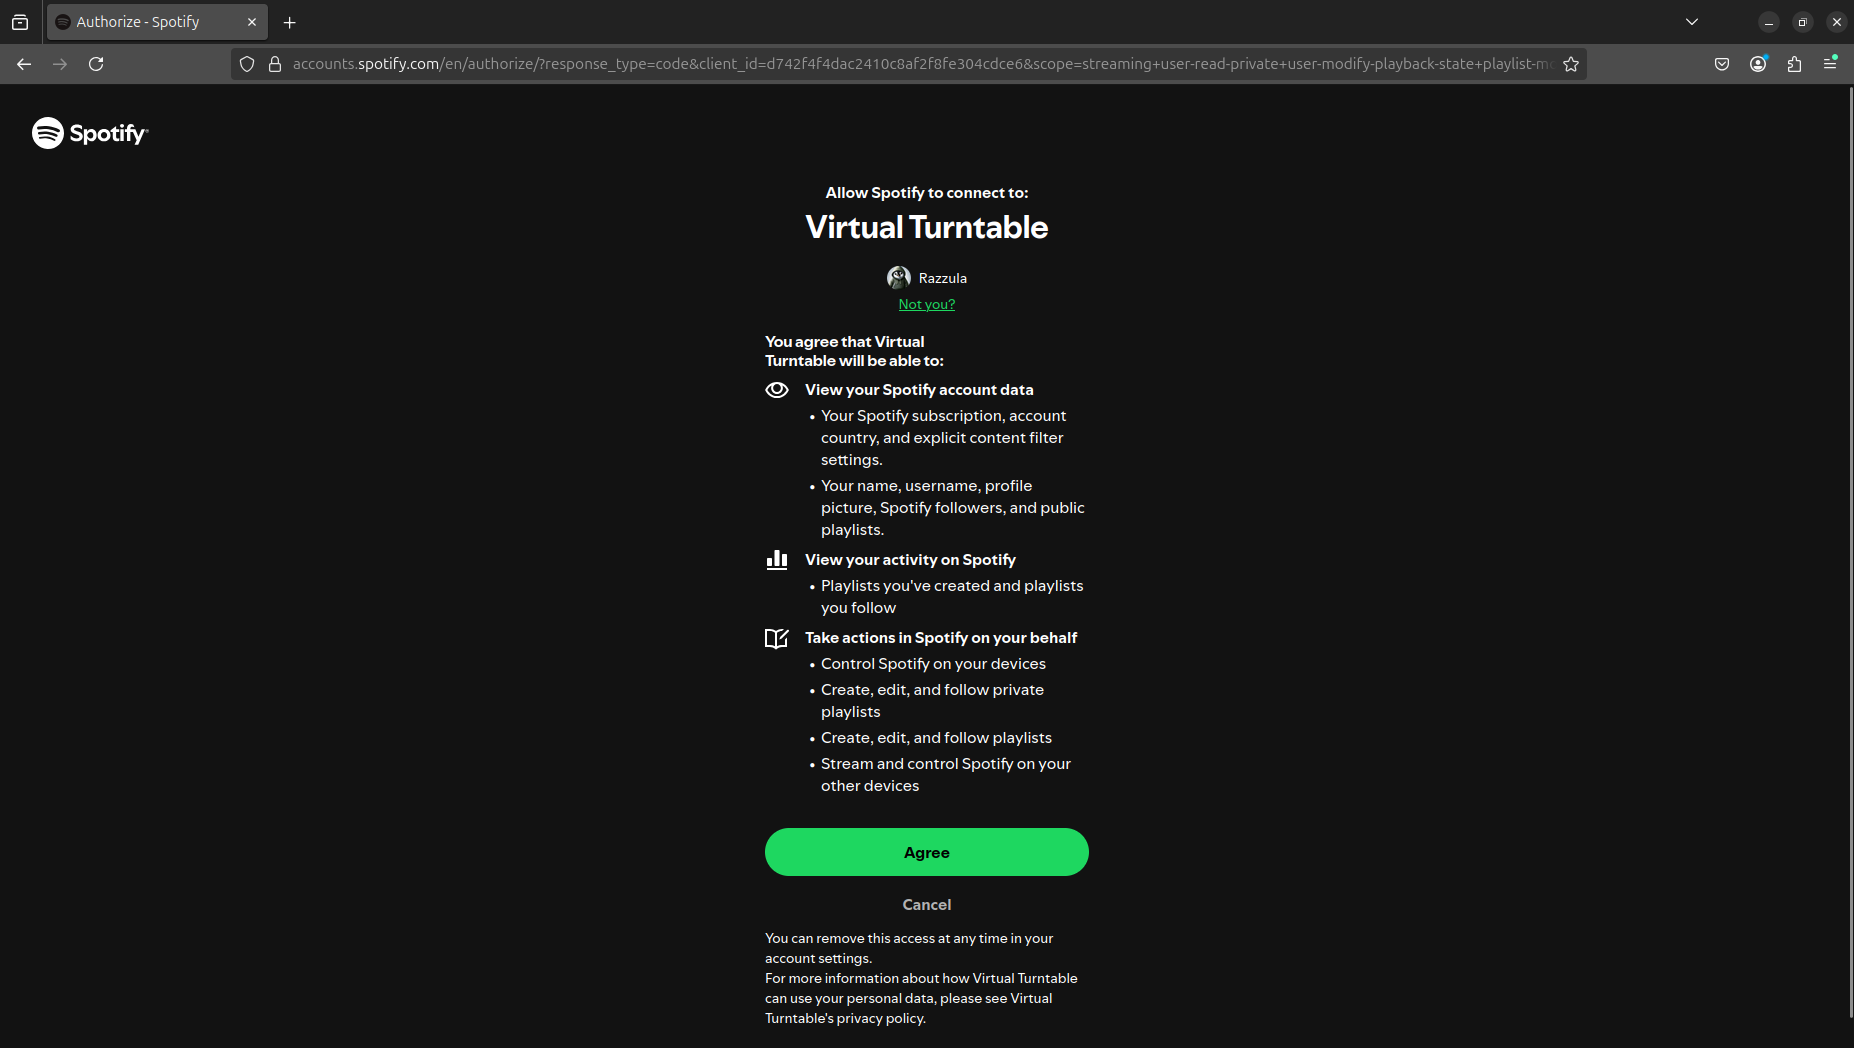
\includegraphics[width=0.4\textwidth]{images/screenshots/HOST_Auth.png}
                \caption{Screenshot of host client using Spotify's authentication redirection flow}
                \label{fig:hostAuth}
            \end{figure}
            
            \begin{figure}[h]
                \centering
                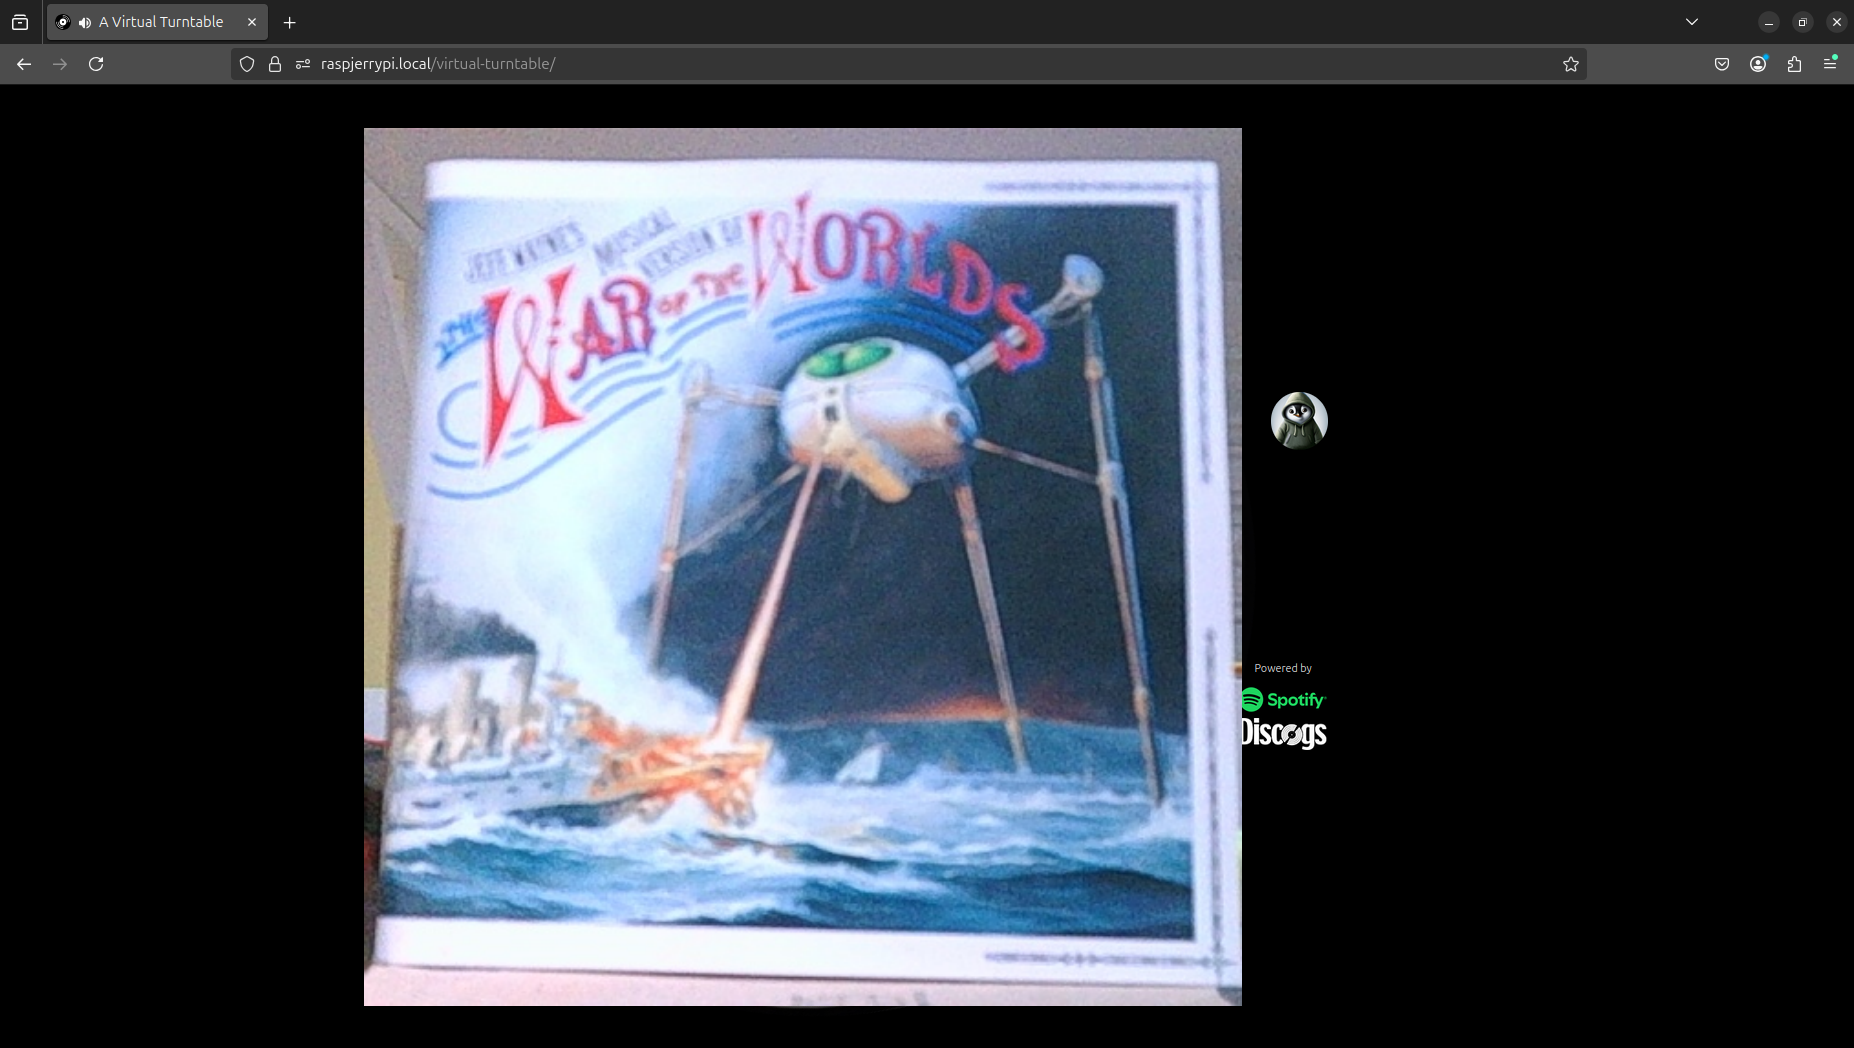
\includegraphics[width=0.4\textwidth]{images/screenshots/HOST_Cam.png}
                \caption{Screenshot of host client displaying the input image from the camera}
                \label{fig:hostCam}
            \end{figure}
            
            \begin{figure}[h]
                \centering
                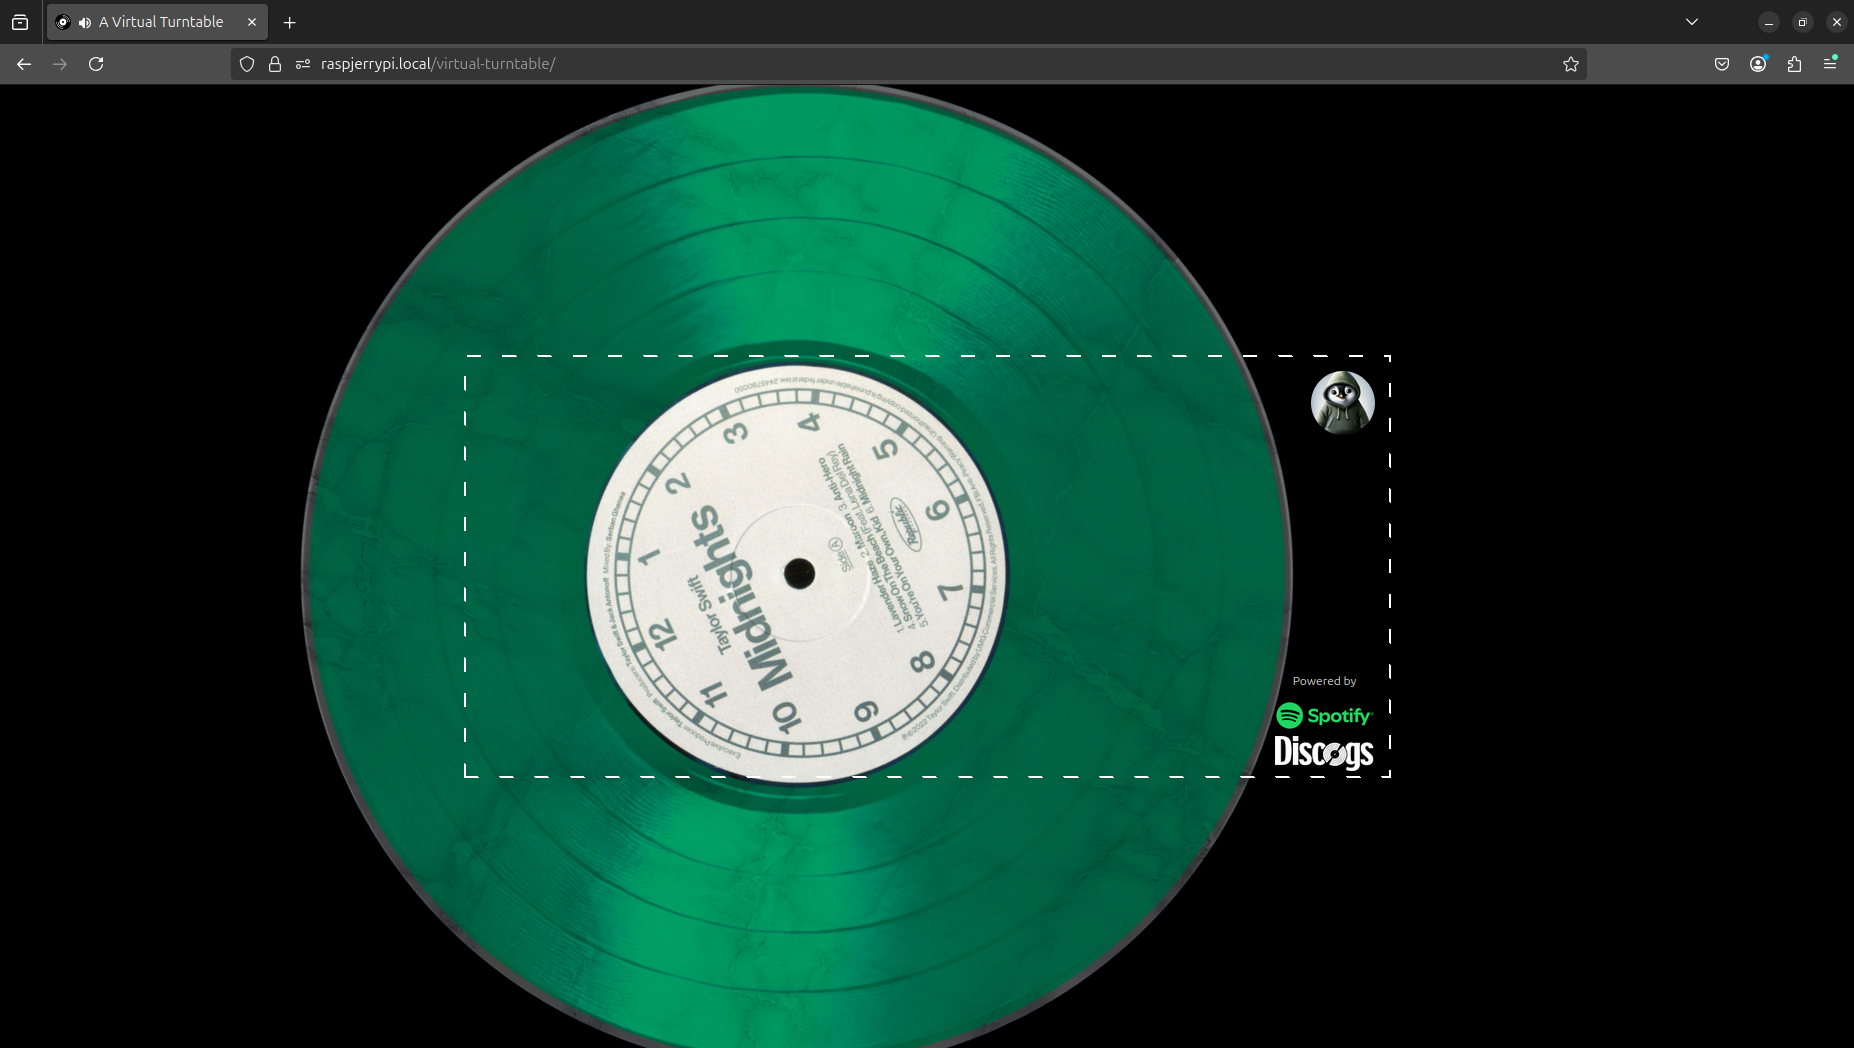
\includegraphics[width=0.4\textwidth]{images/screenshots/HOST_Green.png}
                \caption{Screenshot of host client using adaptive colouring and texturing}
                \label{fig:hostGreen}
            \end{figure}
            
            \begin{figure}[h]
                \centering
                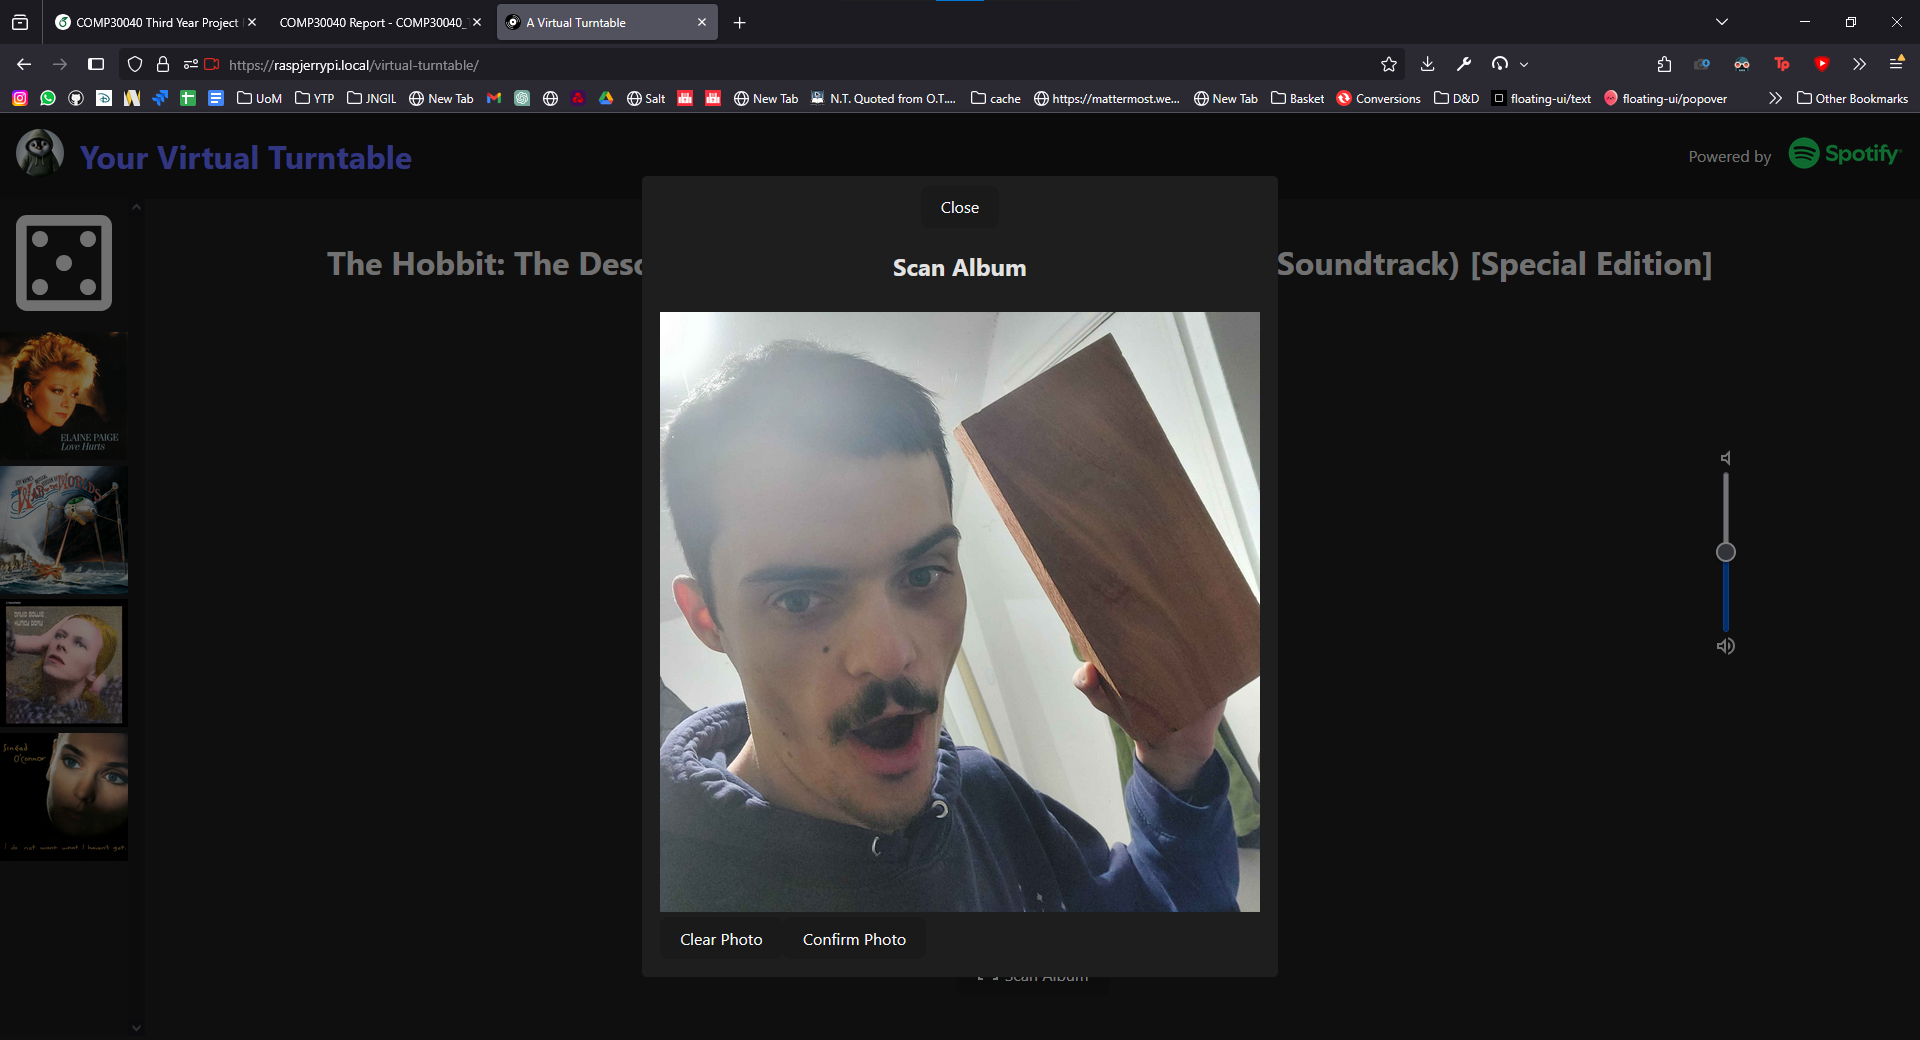
\includegraphics[width=0.4\textwidth]{images/screenshots/LAPTOP_Cam.png}
                \caption{Screenshot of a remote client (PC) using the camera functionality}
                \label{fig:laptopCam}
            \end{figure}
            
            \begin{figure}[h]
                \centering
                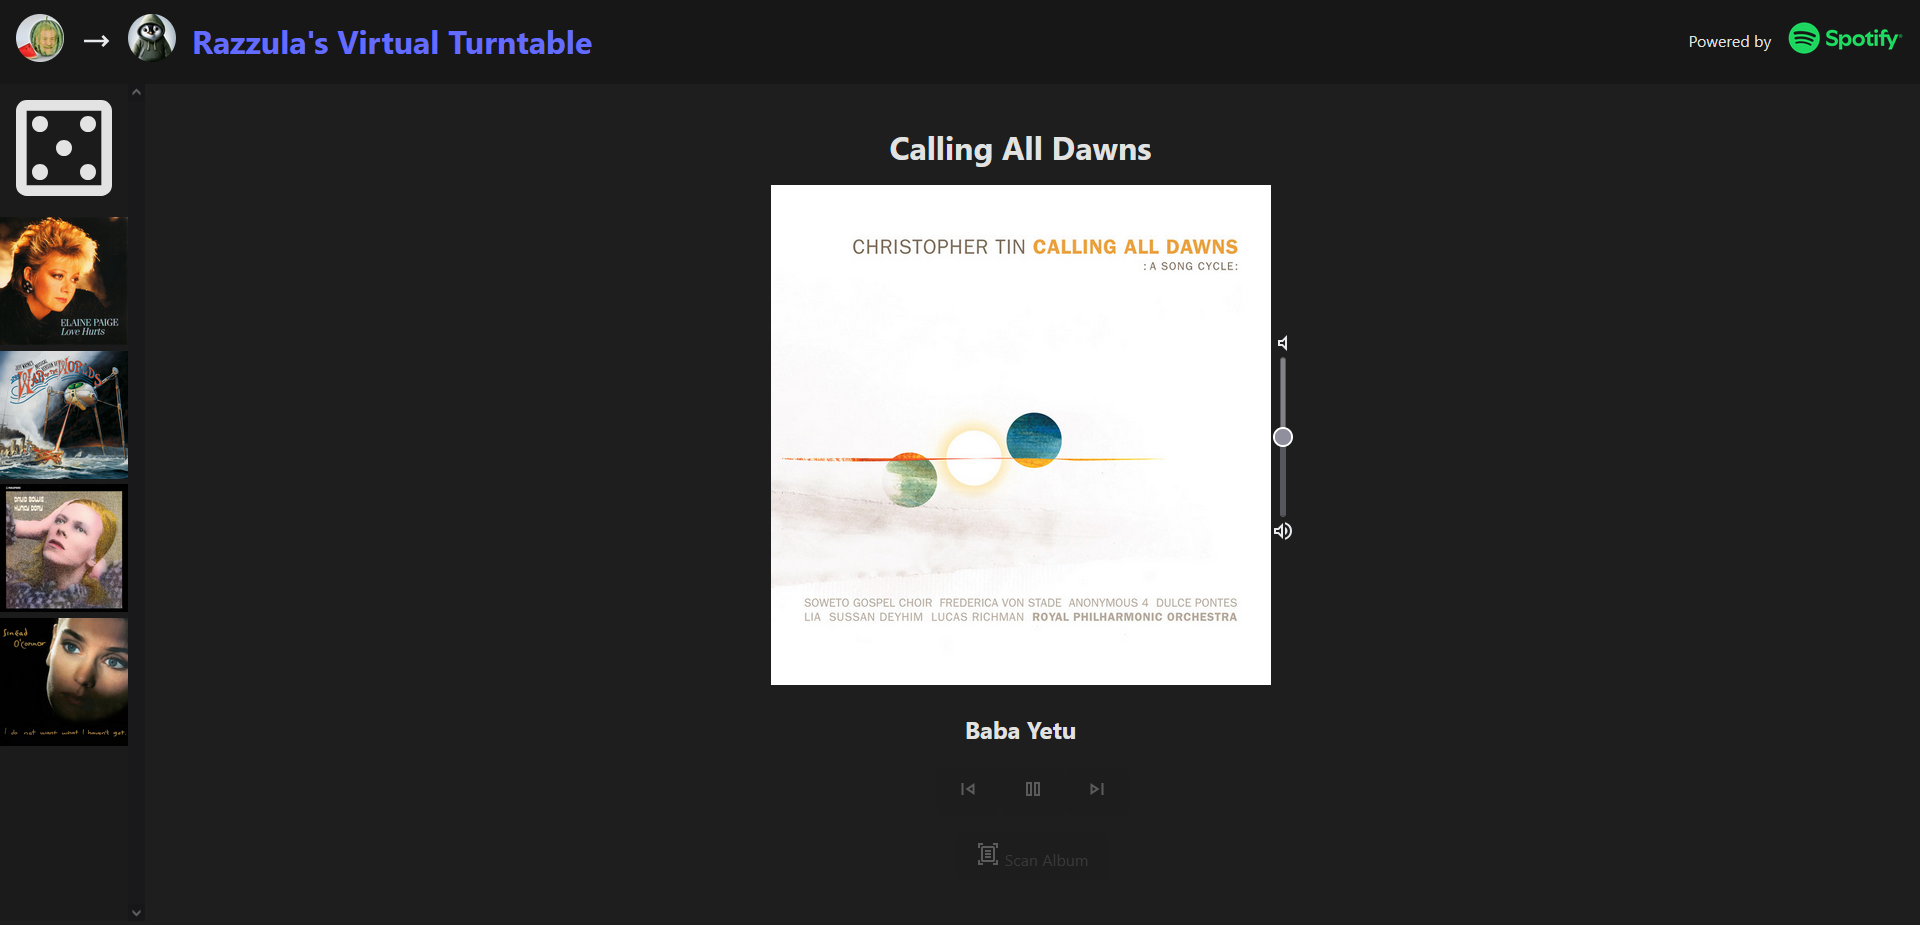
\includegraphics[width=0.4\textwidth]{images/screenshots/LAPTOP_External.png}
                \caption{Screenshot of a remote client, using an external account (not the host)}
                \label{fig:laptopExternal}
            \end{figure}
            
            \begin{figure}[h]
                \centering
                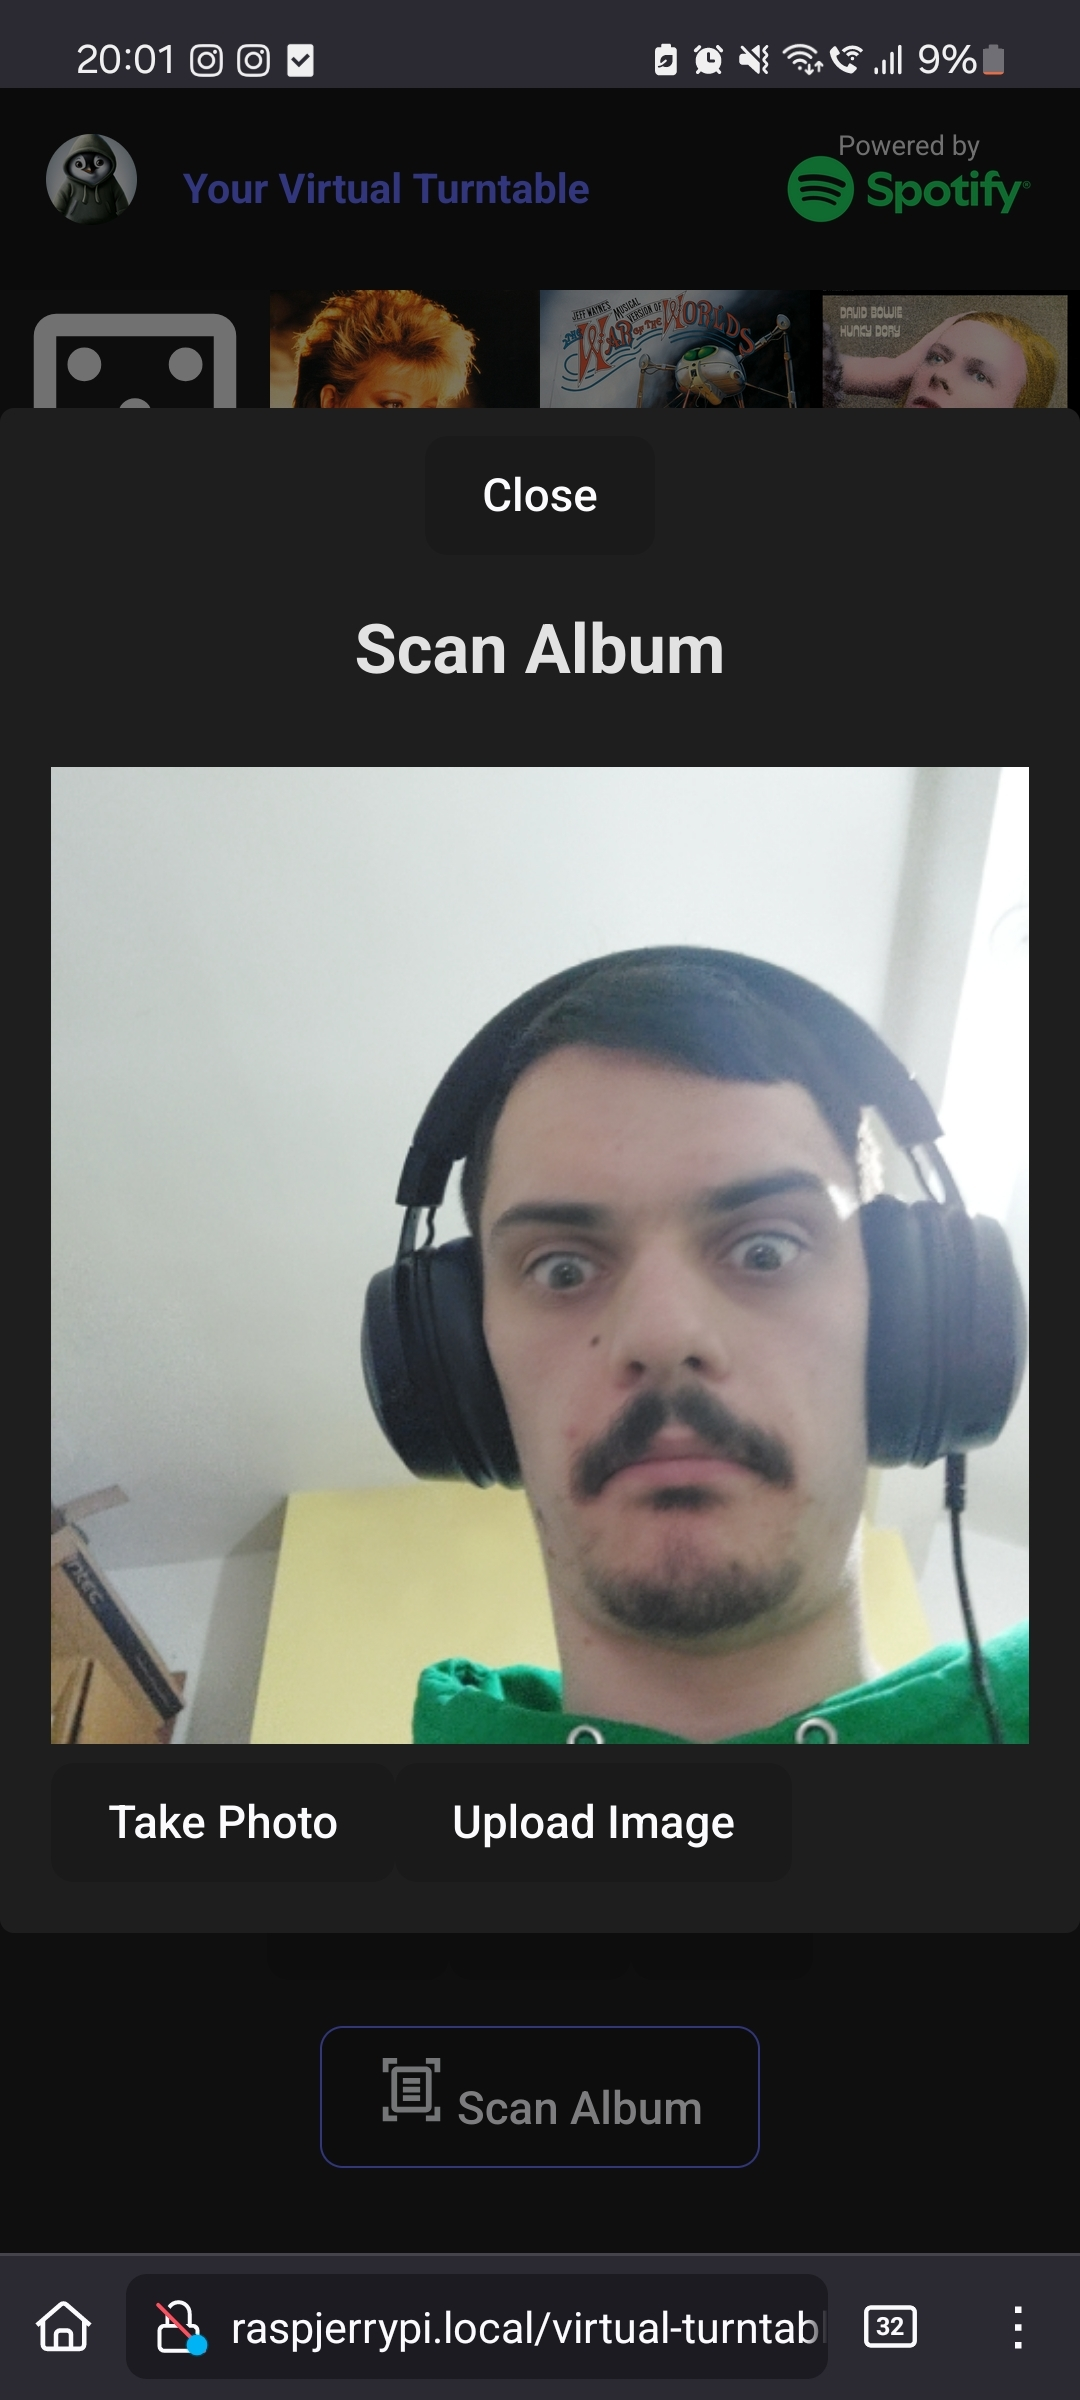
\includegraphics[width=0.4\textwidth]{images/screenshots/PHONE_Cam.jpg}
                \caption{Screenshot of a remote client (mobile) using the camera functionality}
                \label{fig:phoneCam}
            \end{figure}
            
            \begin{figure}[h]
                \centering
                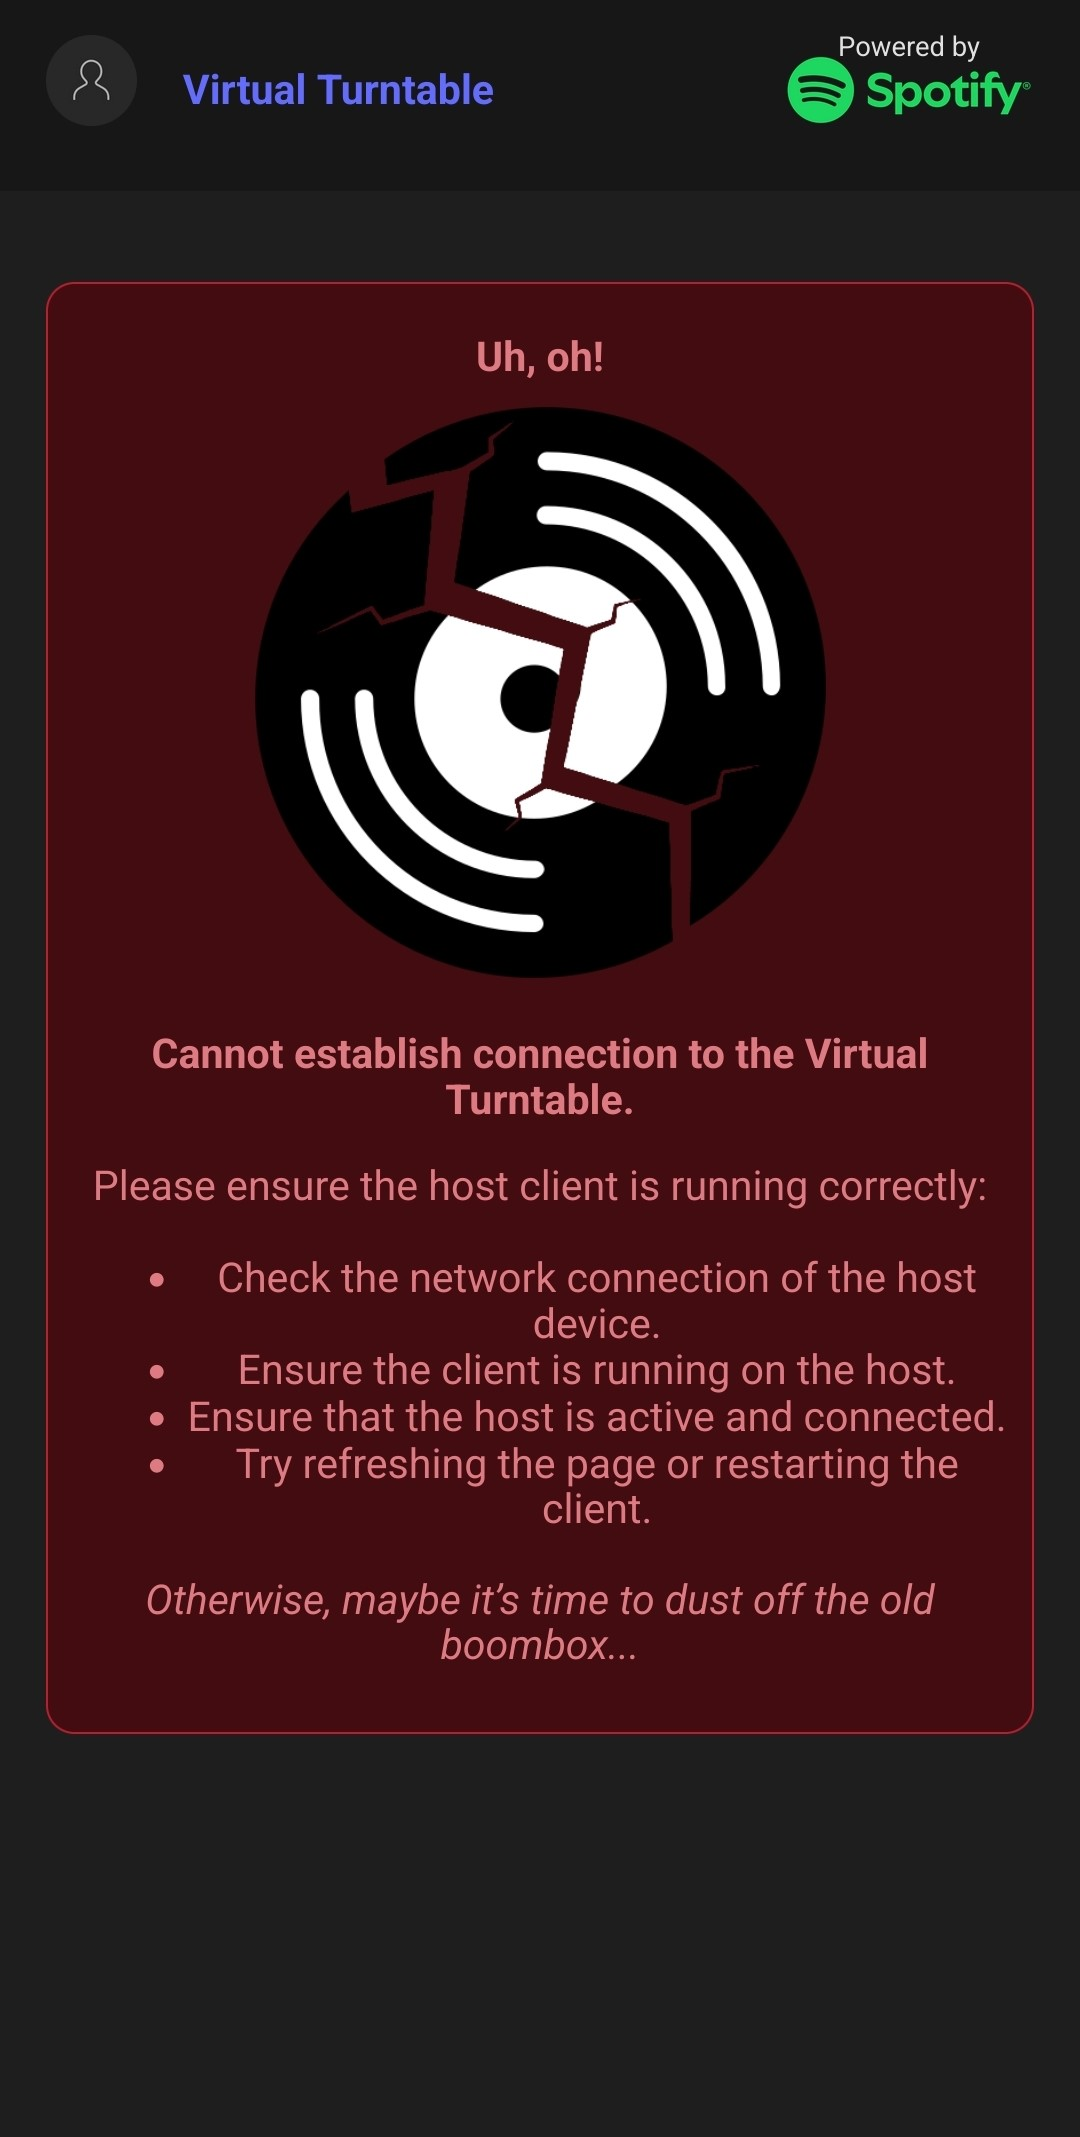
\includegraphics[width=0.4\textwidth]{images/screenshots/PHONE_Error.jpg}
                \caption{Screenshot of a remote client displaying a 404 error}
                \label{fig:phoneError}
            \end{figure}
    
    
        \section{Supplementary Information}
    
            \subsection{Mythological Inspiration} \label{app:Greek}
    
                \paragraph{Ouroboros} A mythological serpent known for circling and eating its own tail, as in Figure \ref{fig:ouroboros}. This name was used for the simple one-headed CNN model design, which 'self-fed' on deployment data with a low-distribution shift between its training data.
    
                \paragraph{Amphisbaena} A snake-like creature, also of origin in Greek mythology, with a notable second head at the end of its tail, as in Figure \ref{fig:amphisbaena}. This creature's name was used for the two-headed neural network design.
    
                \paragraph{Hydra} A rather famous mythological Greek monster, the Hydra of Lerna is a serpentine lake monster, famed for having many heads. These carying number of heads are most well-known for the fact that for every one that was cut off, two more would re-grow in its place. This creature's name was used for the PNN model design, which featured a growing number of heads.
    
                \begin{figure}[h]
                    \centering
                    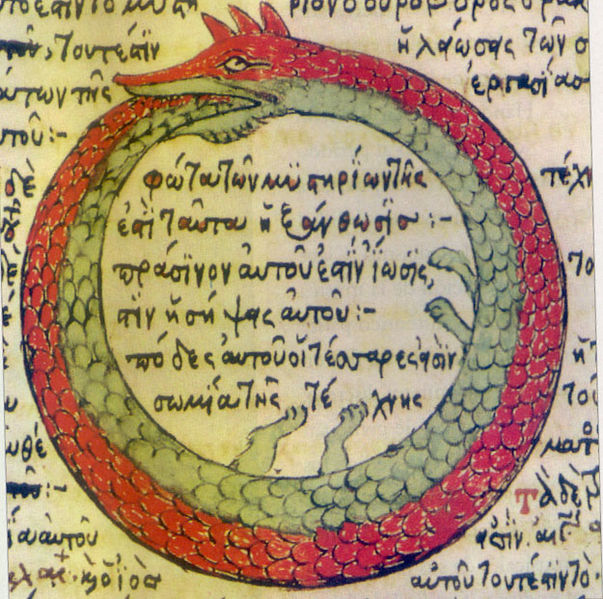
\includegraphics[width=0.6\textwidth]{images/Ouroborus.jpg}
                    \caption{A drawing of an ouroboros, in an alchemical tract (1478)}
                    \label{fig:ouroboros}
                    \caption*{Source: \href{https://en.wikipedia.org/wiki/File:Serpiente_alquimica.jpg}{Wikipedia}}
                \end{figure}
    
                \begin{figure}[h]
                    \centering
                    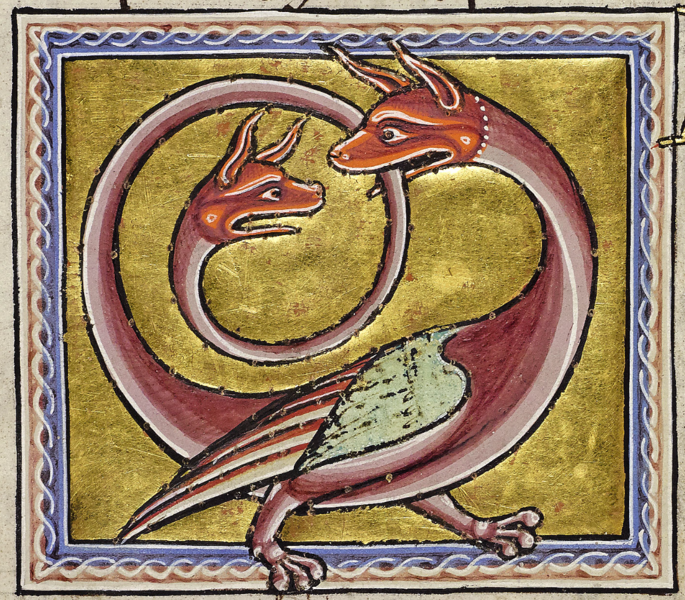
\includegraphics[width=0.6\textwidth]{images/Amphisbaena.png}
                    \caption{An illustration of an amphisbaena (c. 1200)}
                    \label{fig:amphisbaena}
                    \caption*{Source: \href{https://www.abdn.ac.uk/bestiary/ms24/f68v}{The Aberdeen Bestiary, folio 68V.}}
                \end{figure}
    
            \subsection{Cultural Inspiration} \label{app:Cult}
    
                \paragraph{Ed Sheeran Meme} As a light-hearted cultural reference, a meme (Figure~\ref{fig:EdMeme}) highlighting the uniformity of Ed Sheeran’s album art served partially as inspiration for designing a artist classifier. The visual similarity in album covers suggested that artist and album may be decoupled yet jointly learnable.
    
                \begin{figure}[h]
                    \centering
                    
\includegraphics[width=0.6\textwidth]{images/EdSheeranMeme.jpg}
                    \caption{A social media post jokingly referencing the consistent visual theme of Ed Sheeran's album covers}
                    \label{fig:EdMeme}
                    \caption*{Source: \href{https://www.threads.net/@pun_bible/post/DB83pw3gZSh/media}{\@pun\_bible (threads.net)}}
                \end{figure}
        
        %\section{Other appendices as necessary}
    \end{uomappendix}
    
    
    %%%%%%%%%%%%%%%%%% END MATTER %%%%%%%%%%%%%%%%%%
    %TC:endignore
    \end{document}